% Options for packages loaded elsewhere
% Options for packages loaded elsewhere
\PassOptionsToPackage{unicode}{hyperref}
\PassOptionsToPackage{hyphens}{url}
%
\documentclass[
  ignorenonframetext,
  aspectratio=169,
  spanish,
  professionalfonts]{beamer}
\newif\ifbibliography
\usepackage{pgfpages}
\setbeamertemplate{caption}[numbered]
\setbeamertemplate{caption label separator}{: }
\setbeamercolor{caption name}{fg=normal text.fg}
\beamertemplatenavigationsymbolsempty
% remove section numbering
\setbeamertemplate{part page}{
  \centering
  \begin{beamercolorbox}[sep=16pt,center]{part title}
    \usebeamerfont{part title}\insertpart\par
  \end{beamercolorbox}
}
\setbeamertemplate{section page}{
  \centering
  \begin{beamercolorbox}[sep=12pt,center]{section title}
    \usebeamerfont{section title}\insertsection\par
  \end{beamercolorbox}
}
\setbeamertemplate{subsection page}{
  \centering
  \begin{beamercolorbox}[sep=8pt,center]{subsection title}
    \usebeamerfont{subsection title}\insertsubsection\par
  \end{beamercolorbox}
}
% Prevent slide breaks in the middle of a paragraph
\widowpenalties 1 10000
\raggedbottom
\AtBeginPart{
  \frame{\partpage}
}
\AtBeginSection{
  \ifbibliography
  \else
    \frame{\sectionpage}
  \fi
}
\AtBeginSubsection{
  \frame{\subsectionpage}
}
\usepackage{iftex}
\ifPDFTeX
  \usepackage[T1]{fontenc}
  \usepackage[utf8]{inputenc}
  \usepackage{textcomp} % provide euro and other symbols
\else % if luatex or xetex
  \usepackage{unicode-math} % this also loads fontspec
  \defaultfontfeatures{Scale=MatchLowercase}
  \defaultfontfeatures[\rmfamily]{Ligatures=TeX,Scale=1}
\fi
\usepackage{lmodern}

\usetheme[]{Madrid}
\usecolortheme[]{seahorse}
\ifPDFTeX\else
  % xetex/luatex font selection
\fi
% Use upquote if available, for straight quotes in verbatim environments
\IfFileExists{upquote.sty}{\usepackage{upquote}}{}
\IfFileExists{microtype.sty}{% use microtype if available
  \usepackage[]{microtype}
  \UseMicrotypeSet[protrusion]{basicmath} % disable protrusion for tt fonts
}{}
\makeatletter
\@ifundefined{KOMAClassName}{% if non-KOMA class
  \IfFileExists{parskip.sty}{%
    \usepackage{parskip}
  }{% else
    \setlength{\parindent}{0pt}
    \setlength{\parskip}{6pt plus 2pt minus 1pt}}
}{% if KOMA class
  \KOMAoptions{parskip=half}}
\makeatother

\usepackage{color}
\usepackage{fancyvrb}
\newcommand{\VerbBar}{|}
\newcommand{\VERB}{\Verb[commandchars=\\\{\}]}
\DefineVerbatimEnvironment{Highlighting}{Verbatim}{commandchars=\\\{\}}
% Add ',fontsize=\small' for more characters per line
\usepackage{framed}
\definecolor{shadecolor}{RGB}{241,243,245}
\newenvironment{Shaded}{\begin{snugshade}}{\end{snugshade}}
\newcommand{\AlertTok}[1]{\textcolor[rgb]{0.68,0.00,0.00}{#1}}
\newcommand{\AnnotationTok}[1]{\textcolor[rgb]{0.37,0.37,0.37}{#1}}
\newcommand{\AttributeTok}[1]{\textcolor[rgb]{0.40,0.45,0.13}{#1}}
\newcommand{\BaseNTok}[1]{\textcolor[rgb]{0.68,0.00,0.00}{#1}}
\newcommand{\BuiltInTok}[1]{\textcolor[rgb]{0.00,0.23,0.31}{#1}}
\newcommand{\CharTok}[1]{\textcolor[rgb]{0.13,0.47,0.30}{#1}}
\newcommand{\CommentTok}[1]{\textcolor[rgb]{0.37,0.37,0.37}{#1}}
\newcommand{\CommentVarTok}[1]{\textcolor[rgb]{0.37,0.37,0.37}{\textit{#1}}}
\newcommand{\ConstantTok}[1]{\textcolor[rgb]{0.56,0.35,0.01}{#1}}
\newcommand{\ControlFlowTok}[1]{\textcolor[rgb]{0.00,0.23,0.31}{\textbf{#1}}}
\newcommand{\DataTypeTok}[1]{\textcolor[rgb]{0.68,0.00,0.00}{#1}}
\newcommand{\DecValTok}[1]{\textcolor[rgb]{0.68,0.00,0.00}{#1}}
\newcommand{\DocumentationTok}[1]{\textcolor[rgb]{0.37,0.37,0.37}{\textit{#1}}}
\newcommand{\ErrorTok}[1]{\textcolor[rgb]{0.68,0.00,0.00}{#1}}
\newcommand{\ExtensionTok}[1]{\textcolor[rgb]{0.00,0.23,0.31}{#1}}
\newcommand{\FloatTok}[1]{\textcolor[rgb]{0.68,0.00,0.00}{#1}}
\newcommand{\FunctionTok}[1]{\textcolor[rgb]{0.28,0.35,0.67}{#1}}
\newcommand{\ImportTok}[1]{\textcolor[rgb]{0.00,0.46,0.62}{#1}}
\newcommand{\InformationTok}[1]{\textcolor[rgb]{0.37,0.37,0.37}{#1}}
\newcommand{\KeywordTok}[1]{\textcolor[rgb]{0.00,0.23,0.31}{\textbf{#1}}}
\newcommand{\NormalTok}[1]{\textcolor[rgb]{0.00,0.23,0.31}{#1}}
\newcommand{\OperatorTok}[1]{\textcolor[rgb]{0.37,0.37,0.37}{#1}}
\newcommand{\OtherTok}[1]{\textcolor[rgb]{0.00,0.23,0.31}{#1}}
\newcommand{\PreprocessorTok}[1]{\textcolor[rgb]{0.68,0.00,0.00}{#1}}
\newcommand{\RegionMarkerTok}[1]{\textcolor[rgb]{0.00,0.23,0.31}{#1}}
\newcommand{\SpecialCharTok}[1]{\textcolor[rgb]{0.37,0.37,0.37}{#1}}
\newcommand{\SpecialStringTok}[1]{\textcolor[rgb]{0.13,0.47,0.30}{#1}}
\newcommand{\StringTok}[1]{\textcolor[rgb]{0.13,0.47,0.30}{#1}}
\newcommand{\VariableTok}[1]{\textcolor[rgb]{0.07,0.07,0.07}{#1}}
\newcommand{\VerbatimStringTok}[1]{\textcolor[rgb]{0.13,0.47,0.30}{#1}}
\newcommand{\WarningTok}[1]{\textcolor[rgb]{0.37,0.37,0.37}{\textit{#1}}}

\usepackage{longtable,booktabs,array}
\newcounter{none} % for unnumbered tables
\usepackage{calc} % for calculating minipage widths
\usepackage{caption}
% Make caption package work with longtable
\makeatletter
\def\fnum@table{\tablename~\thetable}
\makeatother
\usepackage{graphicx}
\makeatletter
\newsavebox\pandoc@box
\newcommand*\pandocbounded[1]{% scales image to fit in text height/width
  \sbox\pandoc@box{#1}%
  \Gscale@div\@tempa{\textheight}{\dimexpr\ht\pandoc@box+\dp\pandoc@box\relax}%
  \Gscale@div\@tempb{\linewidth}{\wd\pandoc@box}%
  \ifdim\@tempb\p@<\@tempa\p@\let\@tempa\@tempb\fi% select the smaller of both
  \ifdim\@tempa\p@<\p@\scalebox{\@tempa}{\usebox\pandoc@box}%
  \else\usebox{\pandoc@box}%
  \fi%
}
% Set default figure placement to htbp
\def\fps@figure{htbp}
\makeatother


% definitions for citeproc citations
\NewDocumentCommand\citeproctext{}{}
\NewDocumentCommand\citeproc{mm}{%
  \begingroup\def\citeproctext{#2}\cite{#1}\endgroup}
\makeatletter
 % allow citations to break across lines
 \let\@cite@ofmt\@firstofone
 % avoid brackets around text for \cite:
 \def\@biblabel#1{}
 \def\@cite#1#2{{#1\if@tempswa , #2\fi}}
\makeatother
\newlength{\cslhangindent}
\setlength{\cslhangindent}{1.5em}
\newlength{\csllabelwidth}
\setlength{\csllabelwidth}{3em}
\newenvironment{CSLReferences}[2] % #1 hanging-indent, #2 entry-spacing
 {\begin{list}{}{%
  \setlength{\itemindent}{0pt}
  \setlength{\leftmargin}{0pt}
  \setlength{\parsep}{0pt}
  % turn on hanging indent if param 1 is 1
  \ifodd #1
   \setlength{\leftmargin}{\cslhangindent}
   \setlength{\itemindent}{-1\cslhangindent}
  \fi
  % set entry spacing
  \setlength{\itemsep}{#2\baselineskip}}}
 {\end{list}}
\usepackage{calc}
\newcommand{\CSLBlock}[1]{\hfill\break\parbox[t]{\linewidth}{\strut\ignorespaces#1\strut}}
\newcommand{\CSLLeftMargin}[1]{\parbox[t]{\csllabelwidth}{\strut#1\strut}}
\newcommand{\CSLRightInline}[1]{\parbox[t]{\linewidth - \csllabelwidth}{\strut#1\strut}}
\newcommand{\CSLIndent}[1]{\hspace{\cslhangindent}#1}

\ifLuaTeX
\usepackage[bidi=basic,shorthands=off]{babel}
\else
\usepackage[bidi=default,shorthands=off]{babel}
\fi
\ifLuaTeX
  \usepackage{selnolig} % disable illegal ligatures
\fi


\setlength{\emergencystretch}{3em} % prevent overfull lines

\providecommand{\tightlist}{%
  \setlength{\itemsep}{0pt}\setlength{\parskip}{0pt}}



 


\definecolor{SYSBnavy}{HTML}{123047}
\definecolor{SYSBteal}{HTML}{008C86}
\definecolor{SYSBcoral}{HTML}{E76F51}
\setbeamercolor{structure}{fg=SYSBteal}
\setbeamercolor{frametitle}{fg=white,bg=SYSBnavy}
\setbeamercolor{alerted text}{fg=SYSBcoral}
\setbeamertemplate{navigation symbols}{}
\setbeamertemplate{section page}{\begin{centering}\vfill{\usebeamerfont{section title}\usebeamercolor[fg]{section title}\insertsectionhead\par}\vfill\end{centering}}
\makeatletter
\@ifpackageloaded{tcolorbox}{}{\usepackage[skins,breakable]{tcolorbox}}
\@ifpackageloaded{fontawesome5}{}{\usepackage{fontawesome5}}
\definecolor{quarto-callout-color}{HTML}{909090}
\definecolor{quarto-callout-note-color}{HTML}{0758E5}
\definecolor{quarto-callout-important-color}{HTML}{CC1914}
\definecolor{quarto-callout-warning-color}{HTML}{EB9113}
\definecolor{quarto-callout-tip-color}{HTML}{00A047}
\definecolor{quarto-callout-caution-color}{HTML}{FC5300}
\definecolor{quarto-callout-color-frame}{HTML}{acacac}
\definecolor{quarto-callout-note-color-frame}{HTML}{4582ec}
\definecolor{quarto-callout-important-color-frame}{HTML}{d9534f}
\definecolor{quarto-callout-warning-color-frame}{HTML}{f0ad4e}
\definecolor{quarto-callout-tip-color-frame}{HTML}{02b875}
\definecolor{quarto-callout-caution-color-frame}{HTML}{fd7e14}
\makeatother
\makeatletter
\@ifpackageloaded{caption}{}{\usepackage{caption}}
\AtBeginDocument{%
\ifdefined\contentsname
  \renewcommand*\contentsname{Tabla de contenidos}
\else
  \newcommand\contentsname{Tabla de contenidos}
\fi
\ifdefined\listfigurename
  \renewcommand*\listfigurename{Listado de Figuras}
\else
  \newcommand\listfigurename{Listado de Figuras}
\fi
\ifdefined\listtablename
  \renewcommand*\listtablename{Listado de Tablas}
\else
  \newcommand\listtablename{Listado de Tablas}
\fi
\ifdefined\figurename
  \renewcommand*\figurename{Figura}
\else
  \newcommand\figurename{Figura}
\fi
\ifdefined\tablename
  \renewcommand*\tablename{Tabla}
\else
  \newcommand\tablename{Tabla}
\fi
}
\@ifpackageloaded{float}{}{\usepackage{float}}
\floatstyle{ruled}
\@ifundefined{c@chapter}{\newfloat{codelisting}{h}{lop}}{\newfloat{codelisting}{h}{lop}[chapter]}
\floatname{codelisting}{Listado}
\newcommand*\listoflistings{\listof{codelisting}{Listado de Listados}}
\makeatother
\makeatletter
\makeatother
\makeatletter
\@ifpackageloaded{caption}{}{\usepackage{caption}}
\@ifpackageloaded{subcaption}{}{\usepackage{subcaption}}
\makeatother

\usepackage{bookmark}
\IfFileExists{xurl.sty}{\usepackage{xurl}}{} % add URL line breaks if available
\urlstyle{same}
\hypersetup{
  pdftitle={Sistemas y Señales Biomédicos},
  pdfauthor={Ph.D.~Pablo Eduardo Caicedo Rodríguez},
  pdflang={es},
  hidelinks,
  pdfcreator={LaTeX via pandoc}}


\title{\texorpdfstring{Sistemas y Señales
Biomédicos}{Sistemas y Señales Biomédicos}}
\subtitle{\texorpdfstring{Fundamentos, análisis temporal e introducción
a Fourier}{Fundamentos, análisis temporal e introducción a Fourier}}
\author{Ph.D.~Pablo Eduardo Caicedo Rodríguez}
\date{2026-09-11}

\begin{document}
\frame{\titlepage}


\begin{frame}
\end{frame}

\begin{frame}{Cómo estudiar con estas diapositivas}
\protect\phantomsection\label{cuxf3mo-estudiar-con-estas-diapositivas}
\begin{columns}[T]
\begin{column}{0.48\linewidth}
\begin{block}{Antes de cada clase}
\protect\phantomsection\label{antes-de-cada-clase}
\begin{itemize}
\tightlist
\item
  Revise los objetivos y conceptos previos.
\item
  Identifique las variables y sus unidades.
\item
  Intente responder la pregunta inicial.
\end{itemize}
\end{block}
\end{column}

\begin{column}{0.48\linewidth}
\begin{block}{Después de cada clase}
\protect\phantomsection\label{despuuxe9s-de-cada-clase}
\begin{itemize}
\tightlist
\item
  Reproduzca los ejemplos en Python.
\item
  Interprete los resultados fisiológicamente.
\item
  Resuelva las preguntas de verificación sin consultar las respuestas.
\end{itemize}
\end{block}
\end{column}
\end{columns}

\begin{tcolorbox}[enhanced jigsaw, arc=.35mm, bottomrule=.15mm, bottomtitle=1mm, breakable, colback=white, colbacktitle=quarto-callout-warning-color!10!white, colframe=quarto-callout-warning-color-frame, coltitle=black, left=2mm, leftrule=.75mm, opacityback=0, opacitybacktitle=0.6, rightrule=.15mm, title={Alcance}, titlerule=0mm, toprule=.15mm, toptitle=1mm]

Las señales usadas en los ejemplos son sintéticas y tienen propósito
didáctico. No representan registros clínicos ni permiten realizar
diagnósticos.

\end{tcolorbox}
\end{frame}

\section{Semana 1 · Sesión 1}\label{semana-1-sesiuxf3n-1}

\begin{frame}{¿Por qué estudiar señales y sistemas biomédicos?}
\protect\phantomsection\label{por-quuxe9-estudiar-seuxf1ales-y-sistemas-biomuxe9dicos}
Una observación fisiológica puede responder preguntas diferentes:

\begin{itemize}
\tightlist
\item
  \textbf{Descripción:} ¿qué ocurrió durante el registro?
\item
  \textbf{Medición:} ¿cuánto cambió una variable?
\item
  \textbf{Comparación:} ¿existen diferencias entre condiciones?
\item
  \textbf{Monitoreo:} ¿el comportamiento cambia con el tiempo?
\item
  \textbf{Decisión:} ¿la evidencia es suficientemente confiable para
  actuar?
\end{itemize}

\begin{tcolorbox}[enhanced jigsaw, arc=.35mm, bottomrule=.15mm, bottomtitle=1mm, breakable, colback=white, colbacktitle=quarto-callout-important-color!10!white, colframe=quarto-callout-important-color-frame, coltitle=black, left=2mm, leftrule=.75mm, opacityback=0, opacitybacktitle=0.6, rightrule=.15mm, title={Punto central}, titlerule=0mm, toprule=.15mm, toptitle=1mm]

Procesar una bioseñal significa transformar una medición en evidencia
interpretable, conservando la relación con el fenómeno fisiológico que
la originó.

\end{tcolorbox}
\end{frame}

\begin{frame}{Una señal es una función que porta información}
\protect\phantomsection\label{una-seuxf1al-es-una-funciuxf3n-que-porta-informaciuxf3n}
Formalmente, una señal puede expresarse como

\[
x:\mathcal{T}\longrightarrow\mathcal{A},
\]

donde:

\begin{itemize}
\tightlist
\item
  \(\mathcal{T}\) es el dominio de la variable independiente: tiempo,
  posición o índice de muestra.
\item
  \(\mathcal{A}\) es el conjunto de valores posibles: amplitudes
  escalares, vectores o matrices.
\item
  \(x(t)\) o \(x[n]\) relaciona cada instante o muestra con una
  medición.
\end{itemize}

\begin{tcolorbox}[enhanced jigsaw, arc=.35mm, bottomrule=.15mm, bottomtitle=1mm, breakable, colback=white, colbacktitle=quarto-callout-note-color!10!white, colframe=quarto-callout-note-color-frame, coltitle=black, left=2mm, leftrule=.75mm, opacityback=0, opacitybacktitle=0.6, rightrule=.15mm, title={No confunda dato con señal}, titlerule=0mm, toprule=.15mm, toptitle=1mm]

Un valor aislado es un dato. Una señal conserva una \textbf{estructura
de dependencia} respecto al tiempo, al espacio o a otra variable
independiente.

\end{tcolorbox}
\end{frame}

\begin{frame}[shrink]{Las unidades hacen parte del significado}
\protect\phantomsection\label{las-unidades-hacen-parte-del-significado}
{\def\LTcaptype{none} % do not increment counter
\begin{longtable}[]{@{}
  >{\raggedright\arraybackslash}p{(\linewidth - 6\tabcolsep) * \real{0.2500}}
  >{\raggedright\arraybackslash}p{(\linewidth - 6\tabcolsep) * \real{0.2500}}
  >{\raggedright\arraybackslash}p{(\linewidth - 6\tabcolsep) * \real{0.2500}}
  >{\raggedright\arraybackslash}p{(\linewidth - 6\tabcolsep) * \real{0.2500}}@{}}
\toprule\noalign{}
\begin{minipage}[b]{\linewidth}\raggedright
Señal
\end{minipage} & \begin{minipage}[b]{\linewidth}\raggedright
Variable independiente
\end{minipage} & \begin{minipage}[b]{\linewidth}\raggedright
Amplitud habitual
\end{minipage} & \begin{minipage}[b]{\linewidth}\raggedright
Pregunta posible
\end{minipage} \\
\midrule\noalign{}
\endhead
ECG & tiempo (s) & tensión eléctrica (mV) & ¿cómo evoluciona la
actividad eléctrica cardiaca? \\
EMG & tiempo (s) & tensión eléctrica (\(\mu\)V--mV) & ¿cómo cambia la
activación muscular? \\
EEG & tiempo (s) & tensión eléctrica (\(\mu\)V) & ¿qué patrones
oscilatorios aparecen? \\
Respiración & tiempo (s) & flujo, volumen o desplazamiento & ¿cómo varía
el ciclo respiratorio? \\
\bottomrule\noalign{}
\end{longtable}
}

\begin{tcolorbox}[enhanced jigsaw, arc=.35mm, bottomrule=.15mm, bottomtitle=1mm, breakable, colback=white, colbacktitle=quarto-callout-warning-color!10!white, colframe=quarto-callout-warning-color-frame, coltitle=black, left=2mm, leftrule=.75mm, opacityback=0, opacitybacktitle=0.6, rightrule=.15mm, title={Error frecuente}, titlerule=0mm, toprule=.15mm, toptitle=1mm]

Comparar amplitudes sin revisar unidades, ganancia, montaje, sensor y
condiciones de adquisición conduce a conclusiones inválidas.

\end{tcolorbox}
\end{frame}

\begin{frame}[shrink]{Cuatro familias de bioseñales sintéticas}
\protect\phantomsection\label{cuatro-familias-de-bioseuxf1ales-sintuxe9ticas}
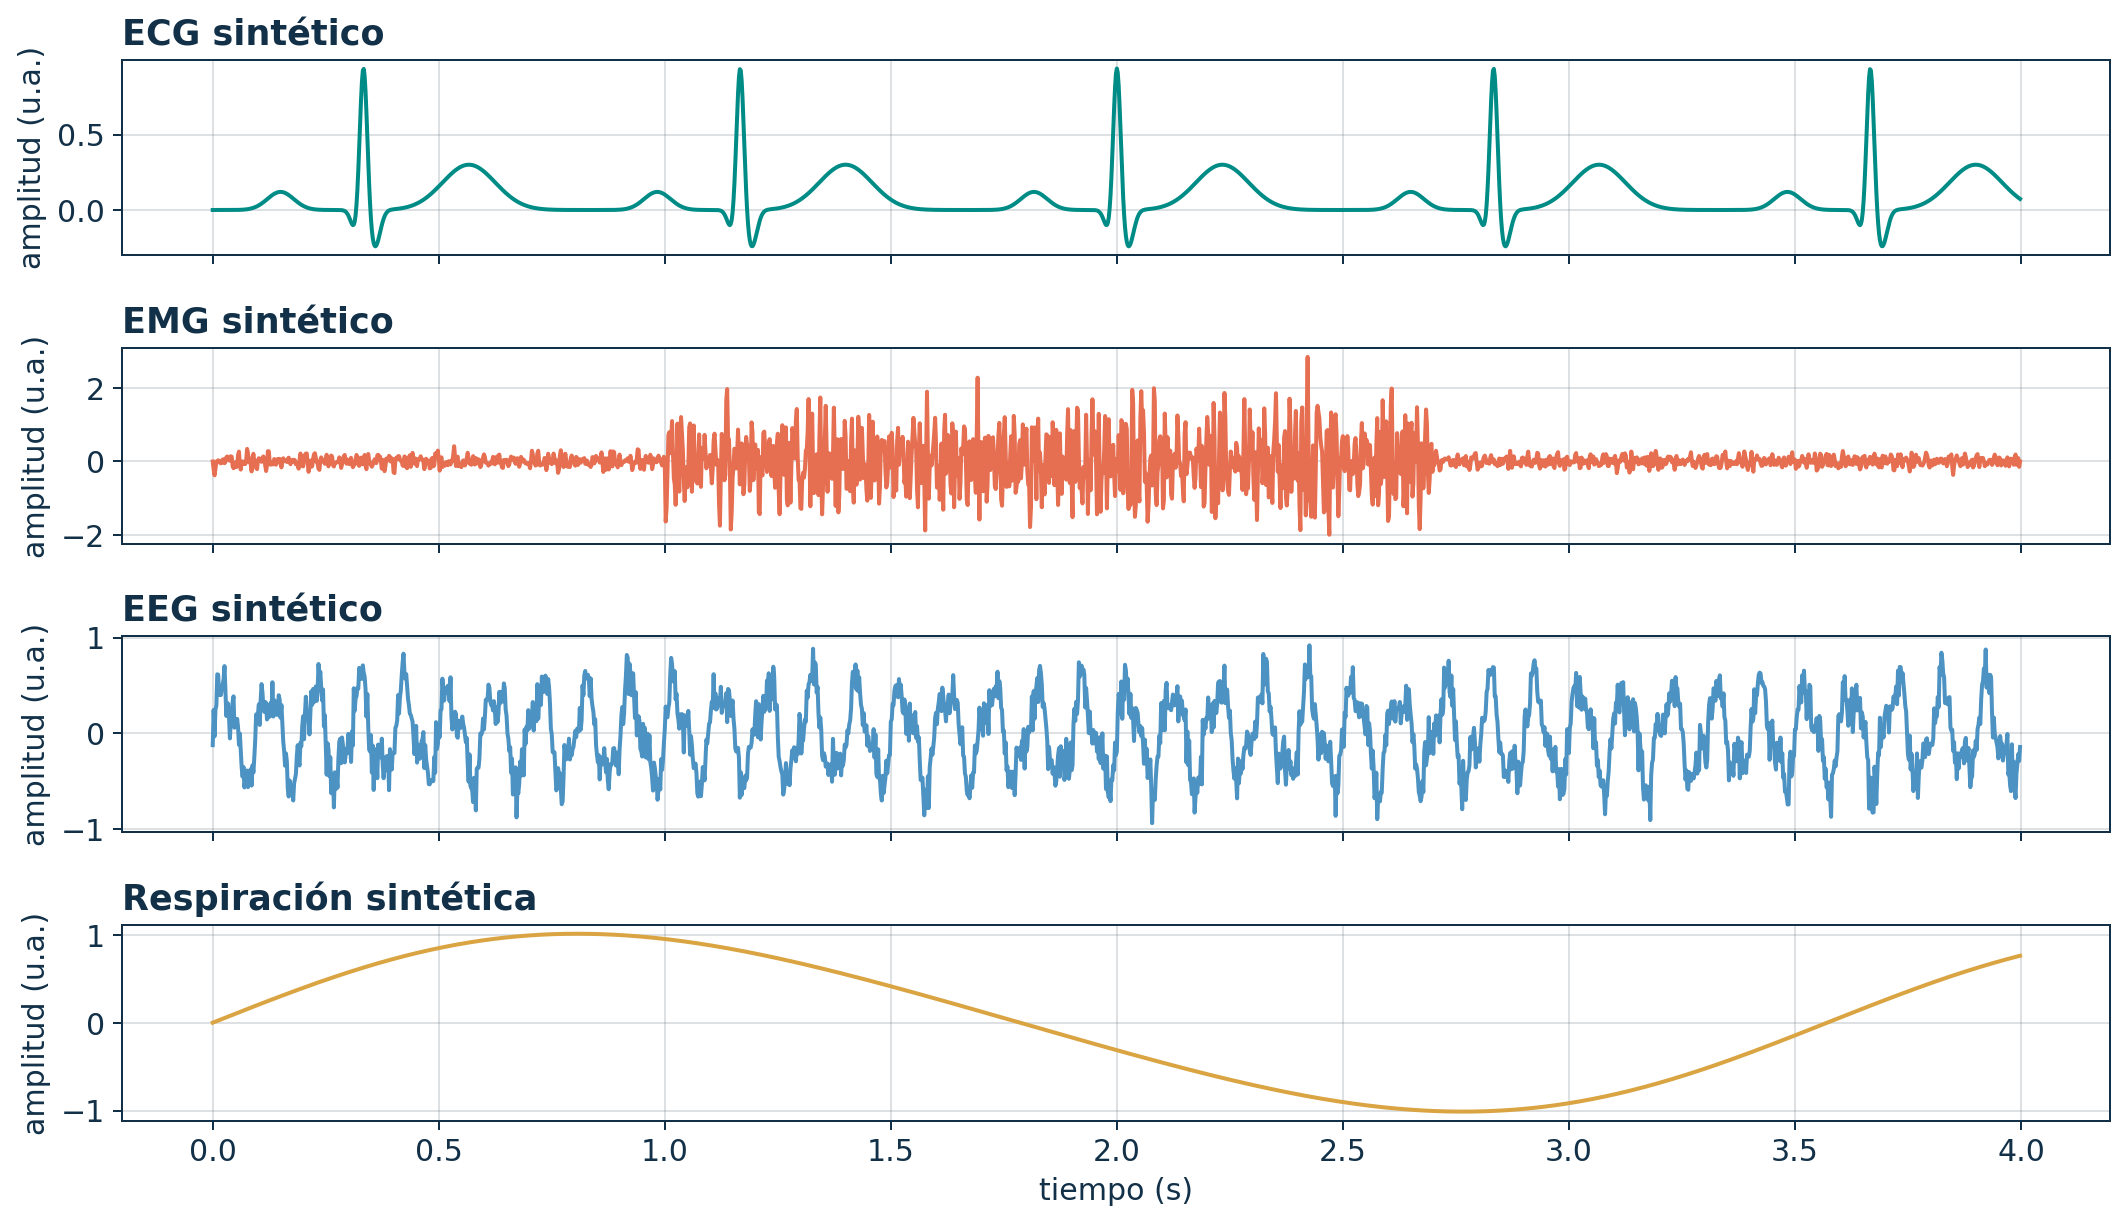
\includegraphics[width=0.84\linewidth,height=\textheight,keepaspectratio]{assets/01_biosignals_overview.png}

\begin{tcolorbox}[enhanced jigsaw, arc=.35mm, bottomrule=.15mm, bottomtitle=1mm, breakable, colback=white, colbacktitle=quarto-callout-tip-color!10!white, colframe=quarto-callout-tip-color-frame, coltitle=black, left=2mm, leftrule=.75mm, opacityback=0, opacitybacktitle=0.6, rightrule=.15mm, title={Lectura de la figura}, titlerule=0mm, toprule=.15mm, toptitle=1mm]

Observe cómo cambian la morfología, la escala temporal y el grado de
aleatoriedad. Esas diferencias orientan la elección de las herramientas
de análisis.

\end{tcolorbox}
\end{frame}

\begin{frame}[shrink]{Del fenómeno fisiológico al dato digital}
\protect\phantomsection\label{del-fenuxf3meno-fisioluxf3gico-al-dato-digital}
{\def\LTcaptype{none} % do not increment counter
\begin{longtable}[]{@{}
  >{\raggedright\arraybackslash}p{(\linewidth - 4\tabcolsep) * \real{0.3333}}
  >{\raggedright\arraybackslash}p{(\linewidth - 4\tabcolsep) * \real{0.3333}}
  >{\raggedright\arraybackslash}p{(\linewidth - 4\tabcolsep) * \real{0.3333}}@{}}
\toprule\noalign{}
\begin{minipage}[b]{\linewidth}\raggedright
Etapa
\end{minipage} & \begin{minipage}[b]{\linewidth}\raggedright
Pregunta de ingeniería
\end{minipage} & \begin{minipage}[b]{\linewidth}\raggedright
Ejemplo
\end{minipage} \\
\midrule\noalign{}
\endhead
\textbf{Fuente} & ¿qué mecanismo genera la variable? & despolarización
celular \\
\textbf{Propagación} & ¿cómo llega hasta la superficie? & conducción
volumétrica \\
\textbf{Sensor} & ¿qué magnitud detecta? & diferencia de potencial \\
\textbf{Acondicionamiento} & ¿cómo se adapta y protege la medición? &
amplificación y filtrado analógico \\
\textbf{Digitalización} & ¿cómo se representa numéricamente? & muestras
y códigos digitales \\
\textbf{Análisis} & ¿qué característica responde la pregunta? &
intervalos, potencia o eventos \\
\bottomrule\noalign{}
\end{longtable}
}

\begin{tcolorbox}[enhanced jigsaw, arc=.35mm, bottomrule=.15mm, bottomtitle=1mm, breakable, colback=white, colbacktitle=quarto-callout-note-color!10!white, colframe=quarto-callout-note-color-frame, coltitle=black, left=2mm, leftrule=.75mm, opacityback=0, opacitybacktitle=0.6, rightrule=.15mm, title={Modelo conceptual}, titlerule=0mm, toprule=.15mm, toptitle=1mm]

El registro depende tanto de la fuente fisiológica como del trayecto de
propagación, del sensor y del sistema de adquisición (Kaniusas 2012).

\end{tcolorbox}
\end{frame}

\begin{frame}{Bioseñal, variable fisiológica y registro no son
sinónimos}
\protect\phantomsection\label{bioseuxf1al-variable-fisioluxf3gica-y-registro-no-son-sinuxf3nimos}
\begin{columns}[T]
\begin{column}{0.48\linewidth}
\begin{block}{Variable fisiológica}
\protect\phantomsection\label{variable-fisioluxf3gica}
Magnitud asociada con un proceso biológico: presión, temperatura,
concentración, actividad eléctrica o movimiento.
\end{block}

\begin{block}{Bioseñal}
\protect\phantomsection\label{bioseuxf1al}
Evolución observable de una variable que porta información del
organismo.
\end{block}
\end{column}

\begin{column}{0.48\linewidth}
\begin{block}{Registro}
\protect\phantomsection\label{registro}
Representación producida por un instrumento bajo condiciones
específicas.
\end{block}

\begin{block}{Característica}
\protect\phantomsection\label{caracteruxedstica}
Cantidad extraída del registro: RMS, intervalo, pendiente, energía o
frecuencia dominante.
\end{block}
\end{column}
\end{columns}

\begin{tcolorbox}[enhanced jigsaw, arc=.35mm, bottomrule=.15mm, bottomtitle=1mm, breakable, colback=white, colbacktitle=quarto-callout-important-color!10!white, colframe=quarto-callout-important-color-frame, coltitle=black, left=2mm, leftrule=.75mm, opacityback=0, opacitybacktitle=0.6, rightrule=.15mm, title={Consecuencia}, titlerule=0mm, toprule=.15mm, toptitle=1mm]

Una característica solo tiene sentido si puede vincularse con una
pregunta fisiológica y con un procedimiento de medición reproducible.

\end{tcolorbox}
\end{frame}

\begin{frame}{El contexto cambia la interpretación}
\protect\phantomsection\label{el-contexto-cambia-la-interpretaciuxf3n}
Una misma amplitud puede tener significados distintos según:

\begin{itemize}
\tightlist
\item
  el tipo y la ubicación del sensor;
\item
  la postura, tarea o condición experimental;
\item
  la frecuencia de muestreo y el ancho de banda;
\item
  la referencia empleada y la ganancia instrumental;
\item
  la presencia de artefactos;
\item
  la población y el objetivo del análisis.
\end{itemize}

\begin{tcolorbox}[enhanced jigsaw, arc=.35mm, bottomrule=.15mm, bottomtitle=1mm, breakable, colback=white, colbacktitle=quarto-callout-caution-color!10!white, colframe=quarto-callout-caution-color-frame, coltitle=black, left=2mm, leftrule=.75mm, opacityback=0, opacitybacktitle=0.6, rightrule=.15mm, title={Criterio crítico}, titlerule=0mm, toprule=.15mm, toptitle=1mm]

Una forma de onda visualmente plausible no garantiza que el registro sea
fisiológicamente válido.

\end{tcolorbox}
\end{frame}

\begin{frame}{Caso orientador: una amplitud EMG aumentó}
\protect\phantomsection\label{caso-orientador-una-amplitud-emg-aumentuxf3}
¿Qué explicaciones deben considerarse antes de atribuir el cambio a una
mayor activación muscular?

\begin{enumerate}
\tightlist
\item
  Cambio real en el reclutamiento neuromuscular.
\item
  Modificación de la posición u orientación de los electrodos.
\item
  Variación de la impedancia de contacto.
\item
  Diferencia de ganancia o escala.
\item
  Contaminación por movimiento o actividad de músculos cercanos.
\end{enumerate}

\begin{tcolorbox}[enhanced jigsaw, arc=.35mm, bottomrule=.15mm, bottomtitle=1mm, breakable, colback=white, colbacktitle=quarto-callout-tip-color!10!white, colframe=quarto-callout-tip-color-frame, coltitle=black, left=2mm, leftrule=.75mm, opacityback=0, opacitybacktitle=0.6, rightrule=.15mm, title={Regla de análisis}, titlerule=0mm, toprule=.15mm, toptitle=1mm]

Antes de interpretar una característica, enumere explicaciones
fisiológicas, instrumentales y computacionales alternativas.

\end{tcolorbox}
\end{frame}

\begin{frame}{Verificación rápida}
\protect\phantomsection\label{verificaciuxf3n-ruxe1pida}
Clasifique cada enunciado como \textbf{variable fisiológica},
\textbf{señal}, \textbf{registro} o \textbf{característica}:

\begin{enumerate}
\tightlist
\item
  Diferencia de potencial almacenada por un electrocardiógrafo.
\item
  Actividad eléctrica resultante de la despolarización cardiaca.
\item
  Intervalo temporal entre dos eventos detectados.
\item
  Variación temporal del flujo respiratorio.
\end{enumerate}

\begin{tcolorbox}[enhanced jigsaw, arc=.35mm, bottomrule=.15mm, bottomtitle=1mm, breakable, colback=white, colbacktitle=quarto-callout-note-color!10!white, colframe=quarto-callout-note-color-frame, coltitle=black, left=2mm, leftrule=.75mm, opacityback=0, opacitybacktitle=0.6, rightrule=.15mm, title={Criterio de respuesta}, titlerule=0mm, toprule=.15mm, toptitle=1mm]

\begin{enumerate}
\tightlist
\item
  Registro. 2. Variable fisiológica. 3. Característica. 4. Señal.
\end{enumerate}

\end{tcolorbox}
\end{frame}

\begin{frame}{Cierre de la sesión 1}
\protect\phantomsection\label{cierre-de-la-sesiuxf3n-1}
\begin{tcolorbox}[enhanced jigsaw, arc=.35mm, bottomrule=.15mm, bottomtitle=1mm, breakable, colback=white, colbacktitle=quarto-callout-important-color!10!white, colframe=quarto-callout-important-color-frame, coltitle=black, left=2mm, leftrule=.75mm, opacityback=0, opacitybacktitle=0.6, rightrule=.15mm, title={Tres ideas que deben permanecer}, titlerule=0mm, toprule=.15mm, toptitle=1mm]

\begin{enumerate}
\tightlist
\item
  Una señal es una función que representa información respecto a una
  variable independiente.\\
\item
  Una bioseñal registrada está condicionada por la fisiología y por la
  cadena de medición.\\
\item
  Ninguna característica debe interpretarse sin unidades, contexto y
  pregunta de análisis.
\end{enumerate}

\end{tcolorbox}

\textbf{Pregunta para enlazar con la sesión siguiente:} si el registro
no contiene únicamente fisiología, ¿cómo distinguimos la información
útil de la contaminación?
\end{frame}

\section{Semana 1 · Sesión 2}\label{semana-1-sesiuxf3n-2}

\begin{frame}[shrink]{Una bioseñal puede codificar distintos fenómenos
físicos}
\protect\phantomsection\label{una-bioseuxf1al-puede-codificar-distintos-fenuxf3menos-fuxedsicos}
{\def\LTcaptype{none} % do not increment counter
\begin{longtable}[]{@{}
  >{\raggedright\arraybackslash}p{(\linewidth - 6\tabcolsep) * \real{0.2500}}
  >{\raggedright\arraybackslash}p{(\linewidth - 6\tabcolsep) * \real{0.2500}}
  >{\raggedright\arraybackslash}p{(\linewidth - 6\tabcolsep) * \real{0.2500}}
  >{\raggedright\arraybackslash}p{(\linewidth - 6\tabcolsep) * \real{0.2500}}@{}}
\toprule\noalign{}
\begin{minipage}[b]{\linewidth}\raggedright
Modalidad
\end{minipage} & \begin{minipage}[b]{\linewidth}\raggedright
Fenómeno
\end{minipage} & \begin{minipage}[b]{\linewidth}\raggedright
Ejemplo
\end{minipage} & \begin{minipage}[b]{\linewidth}\raggedright
Transducción posible
\end{minipage} \\
\midrule\noalign{}
\endhead
Eléctrica & potenciales y corrientes iónicas & ECG, EMG, EEG &
electrodos \\
Mecánica & desplazamiento, fuerza o presión & marcha, pulso arterial &
acelerómetro, celda de carga \\
Acústica & vibración y propagación sonora & fonocardiograma &
micrófono \\
Óptica & absorción, reflexión o dispersión & fotopletismografía & emisor
y fotodetector \\
Química & concentración o actividad molecular & glucosa, pH & biosensor
electroquímico \\
Térmica & intercambio y distribución de calor & temperatura cutánea &
termistor \\
\bottomrule\noalign{}
\end{longtable}
}

\begin{tcolorbox}[enhanced jigsaw, arc=.35mm, bottomrule=.15mm, bottomtitle=1mm, breakable, colback=white, colbacktitle=quarto-callout-note-color!10!white, colframe=quarto-callout-note-color-frame, coltitle=black, left=2mm, leftrule=.75mm, opacityback=0, opacitybacktitle=0.6, rightrule=.15mm, title={Concepto principal}, titlerule=0mm, toprule=.15mm, toptitle=1mm]

El sensor no ``ve'' directamente el estado de salud: responde a una
magnitud física relacionada con un fenómeno biológico.

\end{tcolorbox}
\end{frame}

\begin{frame}{Un sistema transforma entradas en salidas}
\protect\phantomsection\label{un-sistema-transforma-entradas-en-salidas}
Un sistema puede representarse mediante un operador
\(\mathcal{H}\{\cdot\}\):

\[
y(t)=\mathcal{H}\{x(t)\}.
\]

\begin{itemize}
\tightlist
\item
  \(x(t)\): entrada o estímulo observable.
\item
  \(\mathcal{H}\): dinámica, relación o proceso.
\item
  \(y(t)\): respuesta medida.
\end{itemize}

\begin{tcolorbox}[enhanced jigsaw, arc=.35mm, bottomrule=.15mm, bottomtitle=1mm, breakable, colback=white, colbacktitle=quarto-callout-tip-color!10!white, colframe=quarto-callout-tip-color-frame, coltitle=black, left=2mm, leftrule=.75mm, opacityback=0, opacitybacktitle=0.6, rightrule=.15mm, title={Ejemplo biomédico}, titlerule=0mm, toprule=.15mm, toptitle=1mm]

La actividad neural puede actuar como entrada; la activación muscular y
el movimiento articular son respuestas relacionadas, pero no
equivalentes.

\end{tcolorbox}
\end{frame}

\begin{frame}{Los sistemas biológicos contienen estado, realimentación y
variabilidad}
\protect\phantomsection\label{los-sistemas-bioluxf3gicos-contienen-estado-realimentaciuxf3n-y-variabilidad}
Un modelo más realista distingue entrada, estado interno y observación:

\[
\dot{\mathbf{x}}(t)=f\big(\mathbf{x}(t),\mathbf{u}(t),t\big),
\qquad
\mathbf{y}(t)=g\big(\mathbf{x}(t),\mathbf{u}(t),t\big).
\]

\begin{itemize}
\tightlist
\item
  \(\mathbf{u}(t)\): estímulos o entradas.
\item
  \(\mathbf{x}(t)\): variables internas no siempre observables.
\item
  \(\mathbf{y}(t)\): mediciones disponibles.
\end{itemize}

\begin{tcolorbox}[enhanced jigsaw, arc=.35mm, bottomrule=.15mm, bottomtitle=1mm, breakable, colback=white, colbacktitle=quarto-callout-warning-color!10!white, colframe=quarto-callout-warning-color-frame, coltitle=black, left=2mm, leftrule=.75mm, opacityback=0, opacitybacktitle=0.6, rightrule=.15mm, title={Limitación del modelo}, titlerule=0mm, toprule=.15mm, toptitle=1mm]

Una salida similar puede ser producida por estados internos diferentes.
Este problema de \textbf{identificabilidad} impide inferir
automáticamente la causa fisiológica.

\end{tcolorbox}
\end{frame}

\begin{frame}[shrink]{Modelo mínimo de una medición contaminada}
\protect\phantomsection\label{modelo-muxednimo-de-una-mediciuxf3n-contaminada}
Una representación útil es

\[
y(t)=\mathcal{M}\{s(t)\}+n(t)+i(t)+a(t),
\]

donde:

\begin{itemize}
\tightlist
\item
  \(s(t)\): fenómeno fisiológico de interés;
\item
  \(\mathcal{M}\): cadena de medición;
\item
  \(n(t)\): ruido aleatorio;
\item
  \(i(t)\): interferencia estructurada;
\item
  \(a(t)\): artefacto asociado con el procedimiento o el sujeto.
\end{itemize}

\begin{tcolorbox}[enhanced jigsaw, arc=.35mm, bottomrule=.15mm, bottomtitle=1mm, breakable, colback=white, colbacktitle=quarto-callout-important-color!10!white, colframe=quarto-callout-important-color-frame, coltitle=black, left=2mm, leftrule=.75mm, opacityback=0, opacitybacktitle=0.6, rightrule=.15mm, title={Interpretación}, titlerule=0mm, toprule=.15mm, toptitle=1mm]

El procesamiento busca mejorar la utilidad de \(y(t)\) sin destruir la
información de \(s(t)\) ni crear patrones inexistentes.

\end{tcolorbox}
\end{frame}

\begin{frame}[shrink]{La señal observada es una superposición}
\protect\phantomsection\label{la-seuxf1al-observada-es-una-superposiciuxf3n}
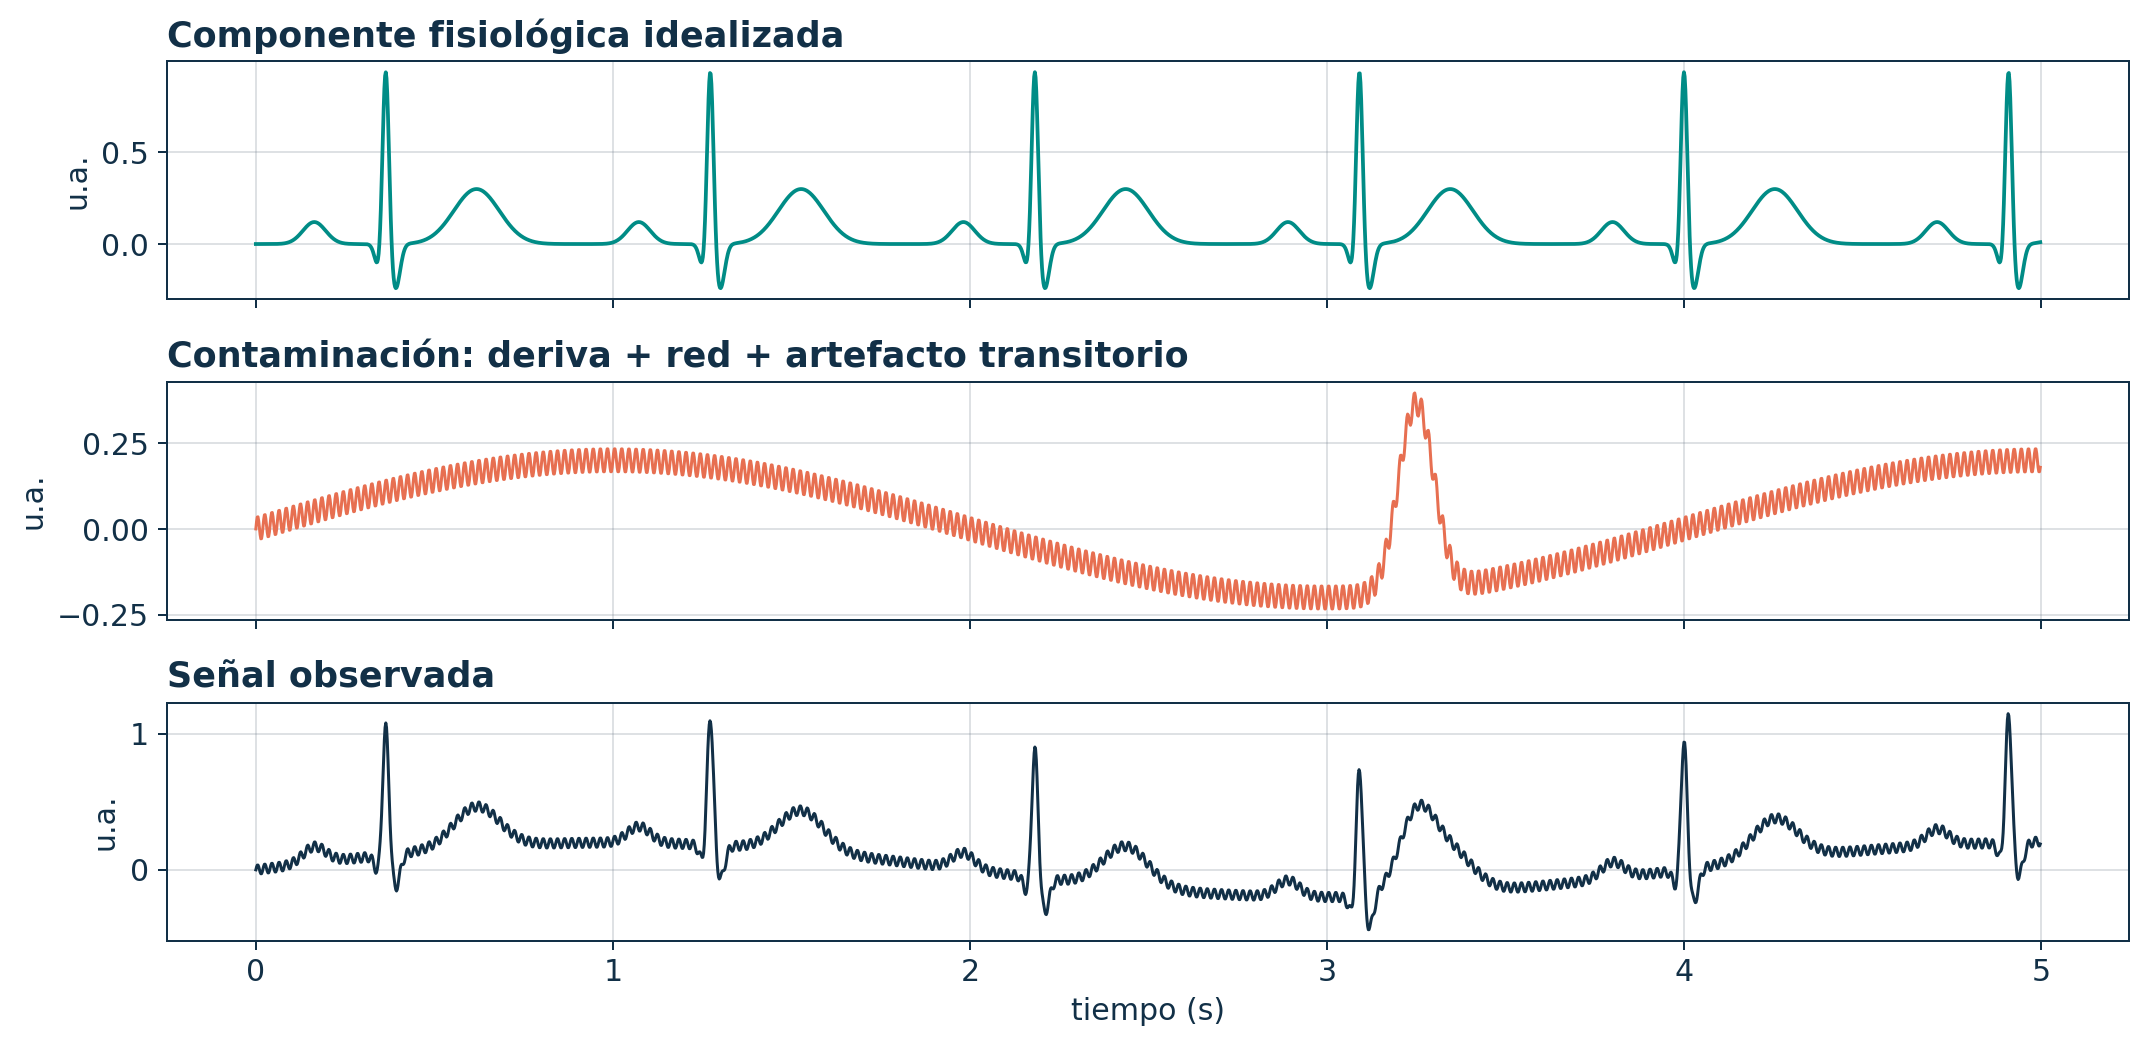
\includegraphics[width=0.84\linewidth,height=\textheight,keepaspectratio]{assets/02_measurement_noise.png}

\begin{tcolorbox}[enhanced jigsaw, arc=.35mm, bottomrule=.15mm, bottomtitle=1mm, breakable, colback=white, colbacktitle=quarto-callout-warning-color!10!white, colframe=quarto-callout-warning-color-frame, coltitle=black, left=2mm, leftrule=.75mm, opacityback=0, opacitybacktitle=0.6, rightrule=.15mm, title={No todo lo indeseado es ruido}, titlerule=0mm, toprule=.15mm, toptitle=1mm]

La deriva de línea base, la interferencia de red y un artefacto de
movimiento tienen estructura diferente; por tanto, requieren estrategias
diferentes.

\end{tcolorbox}
\end{frame}

\begin{frame}[shrink]{Ruido, interferencia y artefacto}
\protect\phantomsection\label{ruido-interferencia-y-artefacto}
{\def\LTcaptype{none} % do not increment counter
\begin{longtable}[]{@{}
  >{\raggedright\arraybackslash}p{(\linewidth - 6\tabcolsep) * \real{0.2500}}
  >{\raggedright\arraybackslash}p{(\linewidth - 6\tabcolsep) * \real{0.2500}}
  >{\raggedright\arraybackslash}p{(\linewidth - 6\tabcolsep) * \real{0.2500}}
  >{\raggedright\arraybackslash}p{(\linewidth - 6\tabcolsep) * \real{0.2500}}@{}}
\toprule\noalign{}
\begin{minipage}[b]{\linewidth}\raggedright
Término
\end{minipage} & \begin{minipage}[b]{\linewidth}\raggedright
Rasgo dominante
\end{minipage} & \begin{minipage}[b]{\linewidth}\raggedright
Ejemplo
\end{minipage} & \begin{minipage}[b]{\linewidth}\raggedright
Pregunta de control
\end{minipage} \\
\midrule\noalign{}
\endhead
\textbf{Ruido} & componente aleatoria & ruido térmico & ¿puede
caracterizarse estadísticamente? \\
\textbf{Interferencia} & fuente externa estructurada & red eléctrica &
¿su frecuencia o forma es reconocible? \\
\textbf{Artefacto} & relación con sujeto o procedimiento & movimiento
del electrodo & ¿coincide con una acción o cambio experimental? \\
\textbf{Variabilidad fisiológica} & cambio real del organismo &
modulación respiratoria & ¿es información que debe conservarse? \\
\bottomrule\noalign{}
\end{longtable}
}

\begin{tcolorbox}[enhanced jigsaw, arc=.35mm, bottomrule=.15mm, bottomtitle=1mm, breakable, colback=white, colbacktitle=quarto-callout-caution-color!10!white, colframe=quarto-callout-caution-color-frame, coltitle=black, left=2mm, leftrule=.75mm, opacityback=0, opacitybacktitle=0.6, rightrule=.15mm, title={Error frecuente}, titlerule=0mm, toprule=.15mm, toptitle=1mm]

Eliminar toda variabilidad puede suprimir precisamente la información
fisiológica que se desea estudiar.

\end{tcolorbox}
\end{frame}

\begin{frame}{Relación señal-ruido}
\protect\phantomsection\label{relaciuxf3n-seuxf1al-ruido}
Si se conocen las potencias de señal y ruido:

\[
\mathrm{SNR}_{\mathrm{dB}}
=10\log_{10}\left(\frac{P_s}{P_n}\right).
\]

Si se comparan valores RMS bajo supuestos compatibles:

\[
\mathrm{SNR}_{\mathrm{dB}}
=20\log_{10}\left(\frac{x_{\mathrm{RMS}}}{n_{\mathrm{RMS}}}\right).
\]

\begin{tcolorbox}[enhanced jigsaw, arc=.35mm, bottomrule=.15mm, bottomtitle=1mm, breakable, colback=white, colbacktitle=quarto-callout-note-color!10!white, colframe=quarto-callout-note-color-frame, coltitle=black, left=2mm, leftrule=.75mm, opacityback=0, opacitybacktitle=0.6, rightrule=.15mm, title={Lectura correcta}, titlerule=0mm, toprule=.15mm, toptitle=1mm]

Una SNR mayor indica mejor separación energética entre señal y ruido; no
demuestra por sí sola que la señal conserve significado fisiológico.

\end{tcolorbox}
\end{frame}

\begin{frame}{La calidad depende de la pregunta}
\protect\phantomsection\label{la-calidad-depende-de-la-pregunta}
Una señal puede ser adecuada para una tarea y deficiente para otra:

\begin{itemize}
\tightlist
\item
  Un ECG puede permitir estimar ritmo, pero no medir con precisión
  segmentos de baja amplitud.
\item
  Un EMG puede detectar el inicio de la contracción, pero no permitir
  comparar amplitudes entre sesiones.
\item
  Un EEG puede mostrar actividad oscilatoria, pero contener artefactos
  que alteran conectividad.
\end{itemize}

\begin{tcolorbox}[enhanced jigsaw, arc=.35mm, bottomrule=.15mm, bottomtitle=1mm, breakable, colback=white, colbacktitle=quarto-callout-important-color!10!white, colframe=quarto-callout-important-color-frame, coltitle=black, left=2mm, leftrule=.75mm, opacityback=0, opacitybacktitle=0.6, rightrule=.15mm, title={Definición operativa}, titlerule=0mm, toprule=.15mm, toptitle=1mm]

La calidad de señal es la capacidad del registro para responder de
manera válida y reproducible una pregunta concreta.

\end{tcolorbox}
\end{frame}

\begin{frame}{Actividad: auditoría de una medición}
\protect\phantomsection\label{actividad-auditoruxeda-de-una-mediciuxf3n}
Seleccione una señal entre ECG, EMG, EEG o respiración y complete:

\begin{enumerate}
\tightlist
\item
  Fuente fisiológica de interés.
\item
  Magnitud física detectada.
\item
  Sensor y ubicación.
\item
  Dos contaminantes plausibles.
\item
  Una característica que respondería la pregunta.
\item
  Una conclusión que \textbf{no} estaría justificada.
\end{enumerate}

\begin{tcolorbox}[enhanced jigsaw, arc=.35mm, bottomrule=.15mm, bottomtitle=1mm, breakable, colback=white, colbacktitle=quarto-callout-tip-color!10!white, colframe=quarto-callout-tip-color-frame, coltitle=black, left=2mm, leftrule=.75mm, opacityback=0, opacitybacktitle=0.6, rightrule=.15mm, title={Criterio de calidad}, titlerule=0mm, toprule=.15mm, toptitle=1mm]

Una buena respuesta separa explícitamente fisiología, adquisición y
procesamiento.

\end{tcolorbox}
\end{frame}

\begin{frame}{Cierre de la semana 1}
\protect\phantomsection\label{cierre-de-la-semana-1}
\begin{tcolorbox}[enhanced jigsaw, arc=.35mm, bottomrule=.15mm, bottomtitle=1mm, breakable, colback=white, colbacktitle=quarto-callout-important-color!10!white, colframe=quarto-callout-important-color-frame, coltitle=black, left=2mm, leftrule=.75mm, opacityback=0, opacitybacktitle=0.6, rightrule=.15mm, title={Síntesis}, titlerule=0mm, toprule=.15mm, toptitle=1mm]

La bioseñal es el resultado de una cadena: \textbf{fuente fisiológica →
propagación → sensor → acondicionamiento → representación digital →
análisis}. Cada etapa introduce supuestos y posibles distorsiones
(Kaniusas 2012; Semmlow y Griffel 2014).

\end{tcolorbox}

\textbf{Preparación para la semana 2:} repase funciones, variables
independientes, vectores, media, varianza y notación de sumatoria.
\end{frame}

\section{Semana 2 · Sesión 1}\label{semana-2-sesiuxf3n-1}

\begin{frame}{Representar una señal es decidir qué se conserva}
\protect\phantomsection\label{representar-una-seuxf1al-es-decidir-quuxe9-se-conserva}
Al finalizar esta sesión podrá:

\begin{itemize}
\tightlist
\item
  distinguir señales continuas y discretas;
\item
  separar continuidad temporal de continuidad en amplitud;
\item
  representar señales escalares y multicanal;
\item
  construir ejes temporales coherentes en Python;
\item
  reconocer cuándo un arreglo numérico todavía carece de contexto
  físico.
\end{itemize}

\begin{tcolorbox}[enhanced jigsaw, arc=.35mm, bottomrule=.15mm, bottomtitle=1mm, breakable, colback=white, colbacktitle=quarto-callout-note-color!10!white, colframe=quarto-callout-note-color-frame, coltitle=black, left=2mm, leftrule=.75mm, opacityback=0, opacitybacktitle=0.6, rightrule=.15mm, title={Pregunta inicial}, titlerule=0mm, toprule=.15mm, toptitle=1mm]

Si dos archivos contienen exactamente los mismos números, ¿representan
necesariamente la misma señal?

\end{tcolorbox}
\end{frame}

\begin{frame}{La variable independiente determina el dominio}
\protect\phantomsection\label{la-variable-independiente-determina-el-dominio}
{\def\LTcaptype{none} % do not increment counter
\begin{longtable}[]{@{}lll@{}}
\toprule\noalign{}
Notación & Dominio & Interpretación \\
\midrule\noalign{}
\endhead
\(x(t)\) & \(t\in\mathbb{R}\) & modelo en tiempo continuo \\
\(x[n]\) & \(n\in\mathbb{Z}\) & secuencia indexada por muestras \\
\(x(\mathbf{r})\) & \(\mathbf{r}\in\mathbb{R}^d\) & señal espacial \\
\(x[m,n]\) & \((m,n)\in\mathbb{Z}^2\) & imagen digital \\
\(\mathbf{x}(t)\) & vector por cada \(t\) & señal multicanal \\
\bottomrule\noalign{}
\end{longtable}
}

\begin{tcolorbox}[enhanced jigsaw, arc=.35mm, bottomrule=.15mm, bottomtitle=1mm, breakable, colback=white, colbacktitle=quarto-callout-important-color!10!white, colframe=quarto-callout-important-color-frame, coltitle=black, left=2mm, leftrule=.75mm, opacityback=0, opacitybacktitle=0.6, rightrule=.15mm, title={Concepto principal}, titlerule=0mm, toprule=.15mm, toptitle=1mm]

La notación comunica qué valores puede tomar la variable independiente.
Cambiar \(t\) por \(n\) no es un detalle tipográfico: cambia el modelo
matemático.

\end{tcolorbox}
\end{frame}

\begin{frame}[shrink]{Tiempo continuo y tiempo discreto}
\protect\phantomsection\label{tiempo-continuo-y-tiempo-discreto}
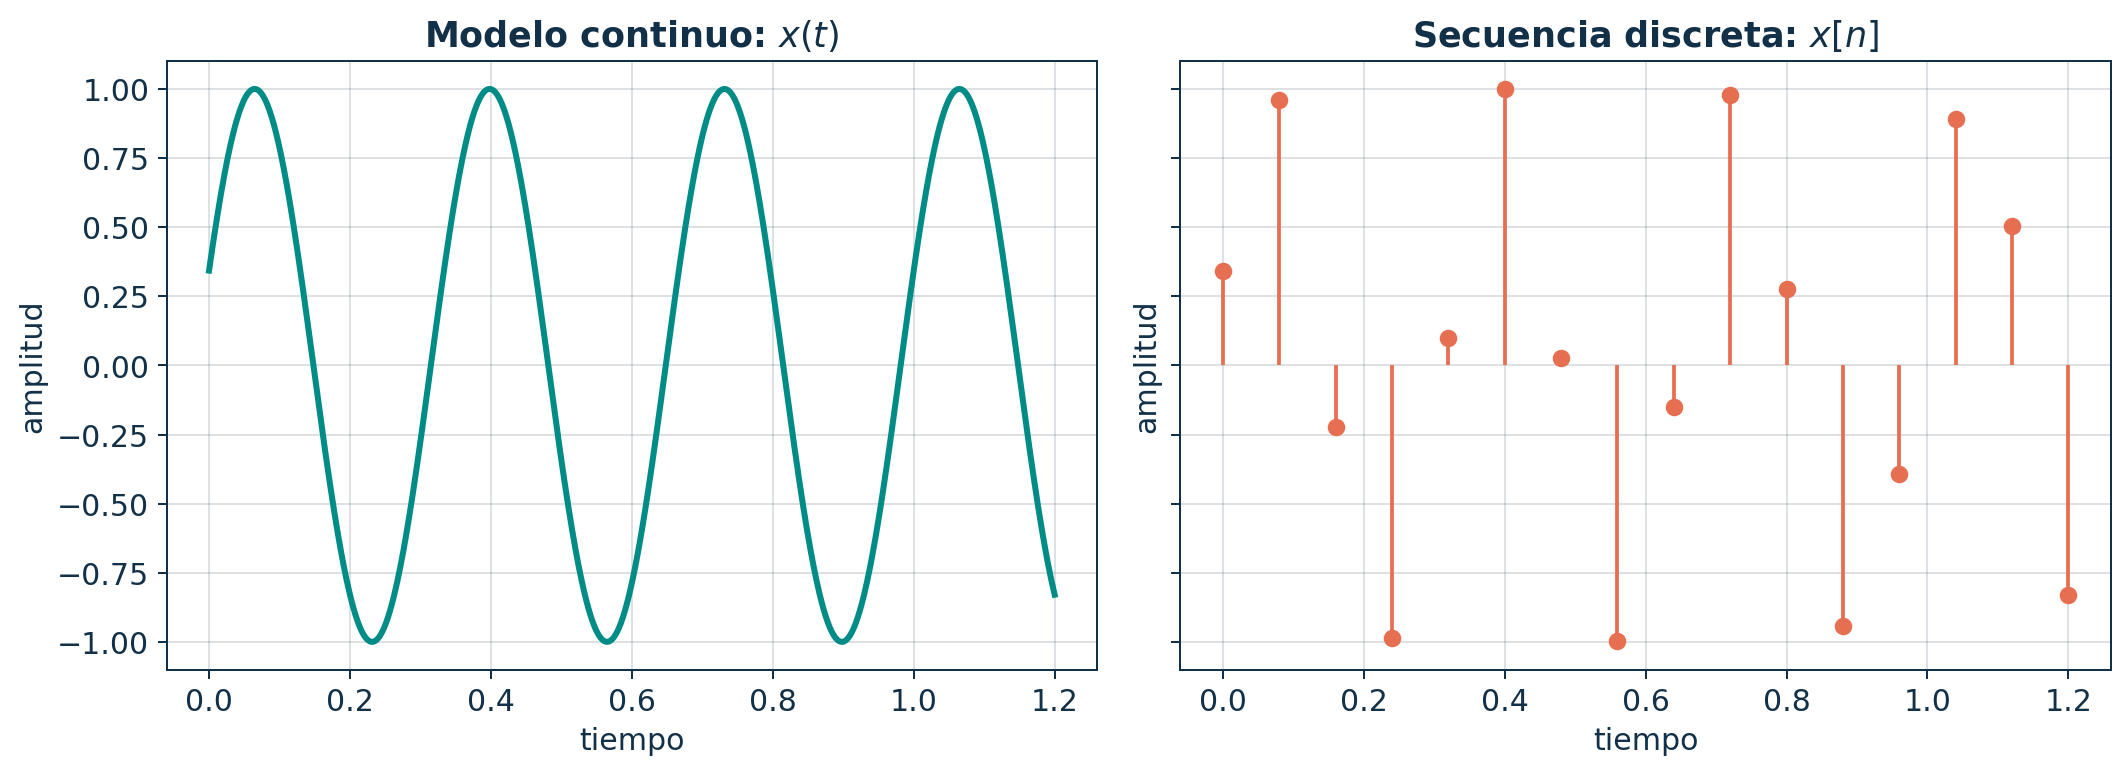
\includegraphics[width=0.84\linewidth,height=\textheight,keepaspectratio]{assets/03_continuous_discrete.png}

\begin{tcolorbox}[enhanced jigsaw, arc=.35mm, bottomrule=.15mm, bottomtitle=1mm, breakable, colback=white, colbacktitle=quarto-callout-note-color!10!white, colframe=quarto-callout-note-color-frame, coltitle=black, left=2mm, leftrule=.75mm, opacityback=0, opacitybacktitle=0.6, rightrule=.15mm, title={Interpretación}, titlerule=0mm, toprule=.15mm, toptitle=1mm]

La curva continua representa un valor para todo \(t\) del intervalo. La
secuencia solo está definida en índices enteros o instantes de muestreo.

\end{tcolorbox}
\end{frame}

\begin{frame}{Cuatro combinaciones que suelen confundirse}
\protect\phantomsection\label{cuatro-combinaciones-que-suelen-confundirse}
{\def\LTcaptype{none} % do not increment counter
\begin{longtable}[]{@{}
  >{\raggedright\arraybackslash}p{(\linewidth - 6\tabcolsep) * \real{0.2500}}
  >{\raggedright\arraybackslash}p{(\linewidth - 6\tabcolsep) * \real{0.2500}}
  >{\raggedright\arraybackslash}p{(\linewidth - 6\tabcolsep) * \real{0.2500}}
  >{\raggedright\arraybackslash}p{(\linewidth - 6\tabcolsep) * \real{0.2500}}@{}}
\toprule\noalign{}
\begin{minipage}[b]{\linewidth}\raggedright
Tiempo
\end{minipage} & \begin{minipage}[b]{\linewidth}\raggedright
Amplitud
\end{minipage} & \begin{minipage}[b]{\linewidth}\raggedright
Representación
\end{minipage} & \begin{minipage}[b]{\linewidth}\raggedright
Ejemplo conceptual
\end{minipage} \\
\midrule\noalign{}
\endhead
continuo & continua & señal analógica ideal & tensión antes del
convertidor \\
discreto & continua & muestras sin cuantizar & modelo matemático del
muestreo \\
continuo & discreta & cambio entre niveles & señal binaria idealizada \\
discreto & discreta & señal digital & códigos almacenados \\
\bottomrule\noalign{}
\end{longtable}
}

\begin{tcolorbox}[enhanced jigsaw, arc=.35mm, bottomrule=.15mm, bottomtitle=1mm, breakable, colback=white, colbacktitle=quarto-callout-warning-color!10!white, colframe=quarto-callout-warning-color-frame, coltitle=black, left=2mm, leftrule=.75mm, opacityback=0, opacitybacktitle=0.6, rightrule=.15mm, title={Error frecuente}, titlerule=0mm, toprule=.15mm, toptitle=1mm]

``Discreta'' puede referirse al dominio temporal o a los niveles de
amplitud. Para evitar ambigüedad, indique cuál de los dos está
discretizado.

\end{tcolorbox}
\end{frame}

\begin{frame}[fragile]{Índice de muestra y tiempo físico}
\protect\phantomsection\label{uxedndice-de-muestra-y-tiempo-fuxedsico}
Si la frecuencia de muestreo es \(f_s\), el intervalo entre muestras es

\[
T_s=\frac{1}{f_s},
\]

y la muestra \(n\) corresponde al instante

\[
t_n=nT_s=\frac{n}{f_s}.
\]

\begin{tcolorbox}[enhanced jigsaw, arc=.35mm, bottomrule=.15mm, bottomtitle=1mm, breakable, colback=white, colbacktitle=quarto-callout-important-color!10!white, colframe=quarto-callout-important-color-frame, coltitle=black, left=2mm, leftrule=.75mm, opacityback=0, opacitybacktitle=0.6, rightrule=.15mm, title={Consecuencia}, titlerule=0mm, toprule=.15mm, toptitle=1mm]

El arreglo \texttt{x} contiene amplitudes; para interpretar duración,
latencia o frecuencia también se necesita conocer \(f_s\).

\end{tcolorbox}
\end{frame}

\begin{frame}[fragile]{Construir correctamente el eje temporal en
Python}
\protect\phantomsection\label{construir-correctamente-el-eje-temporal-en-python}
\begin{Shaded}
\begin{Highlighting}[]
\ImportTok{import}\NormalTok{ numpy }\ImportTok{as}\NormalTok{ np}

\NormalTok{fs }\OperatorTok{=} \DecValTok{500}                 \CommentTok{\# muestras por segundo}
\NormalTok{duration }\OperatorTok{=} \FloatTok{4.0}           \CommentTok{\# segundos}
\NormalTok{n }\OperatorTok{=}\NormalTok{ np.arange(}\BuiltInTok{int}\NormalTok{(fs }\OperatorTok{*}\NormalTok{ duration))}
\NormalTok{t }\OperatorTok{=}\NormalTok{ n }\OperatorTok{/}\NormalTok{ fs               }\CommentTok{\# tiempo físico de cada muestra}

\NormalTok{x }\OperatorTok{=}\NormalTok{ np.sin(}\DecValTok{2} \OperatorTok{*}\NormalTok{ np.pi }\OperatorTok{*} \DecValTok{10} \OperatorTok{*}\NormalTok{ t)}
\BuiltInTok{print}\NormalTok{(x.shape, t[}\OperatorTok{{-}}\DecValTok{1}\NormalTok{])}
\end{Highlighting}
\end{Shaded}

\begin{tcolorbox}[enhanced jigsaw, arc=.35mm, bottomrule=.15mm, bottomtitle=1mm, breakable, colback=white, colbacktitle=quarto-callout-warning-color!10!white, colframe=quarto-callout-warning-color-frame, coltitle=black, left=2mm, leftrule=.75mm, opacityback=0, opacitybacktitle=0.6, rightrule=.15mm, title={Detalle importante}, titlerule=0mm, toprule=.15mm, toptitle=1mm]

Con \texttt{N\ =\ fs*duration}, el último instante es \((N-1)/f_s\), no
exactamente \texttt{duration}.

\end{tcolorbox}
\end{frame}

\begin{frame}{Una señal digital necesita metadatos}
\protect\phantomsection\label{una-seuxf1al-digital-necesita-metadatos}
Un registro reproducible debería especificar, como mínimo:

\begin{itemize}
\tightlist
\item
  frecuencia de muestreo y unidad temporal;
\item
  unidad de amplitud y factor de escala;
\item
  número, nombre y orden de canales;
\item
  sistema de referencia o montaje;
\item
  fecha, condición y duración de adquisición;
\item
  valores ausentes, saturaciones o segmentos excluidos.
\end{itemize}

\begin{tcolorbox}[enhanced jigsaw, arc=.35mm, bottomrule=.15mm, bottomtitle=1mm, breakable, colback=white, colbacktitle=quarto-callout-caution-color!10!white, colframe=quarto-callout-caution-color-frame, coltitle=black, left=2mm, leftrule=.75mm, opacityback=0, opacitybacktitle=0.6, rightrule=.15mm, title={Contrato de datos}, titlerule=0mm, toprule=.15mm, toptitle=1mm]

Sin metadatos, un vector es una secuencia de números; no una medición
biomédica interpretable.

\end{tcolorbox}
\end{frame}

\begin{frame}{Señales escalares y vectoriales}
\protect\phantomsection\label{seuxf1ales-escalares-y-vectoriales}
Una señal escalar asigna un valor a cada instante:

\[x(t)\in\mathbb{R}.\]

Una señal de \(M\) canales asigna un vector:

\[
\mathbf{x}(t)=
\begin{bmatrix}
x_1(t)&x_2(t)&\cdots&x_M(t)
\end{bmatrix}^{\mathsf T}.
\]

\begin{tcolorbox}[enhanced jigsaw, arc=.35mm, bottomrule=.15mm, bottomtitle=1mm, breakable, colback=white, colbacktitle=quarto-callout-note-color!10!white, colframe=quarto-callout-note-color-frame, coltitle=black, left=2mm, leftrule=.75mm, opacityback=0, opacitybacktitle=0.6, rightrule=.15mm, title={Ejemplos}, titlerule=0mm, toprule=.15mm, toptitle=1mm]

Un ECG de varias derivaciones, un EEG multicanal y una plataforma de
fuerza producen observaciones vectoriales.

\end{tcolorbox}
\end{frame}

\begin{frame}[shrink]{Los canales no son repeticiones de la misma señal}
\protect\phantomsection\label{los-canales-no-son-repeticiones-de-la-misma-seuxf1al}
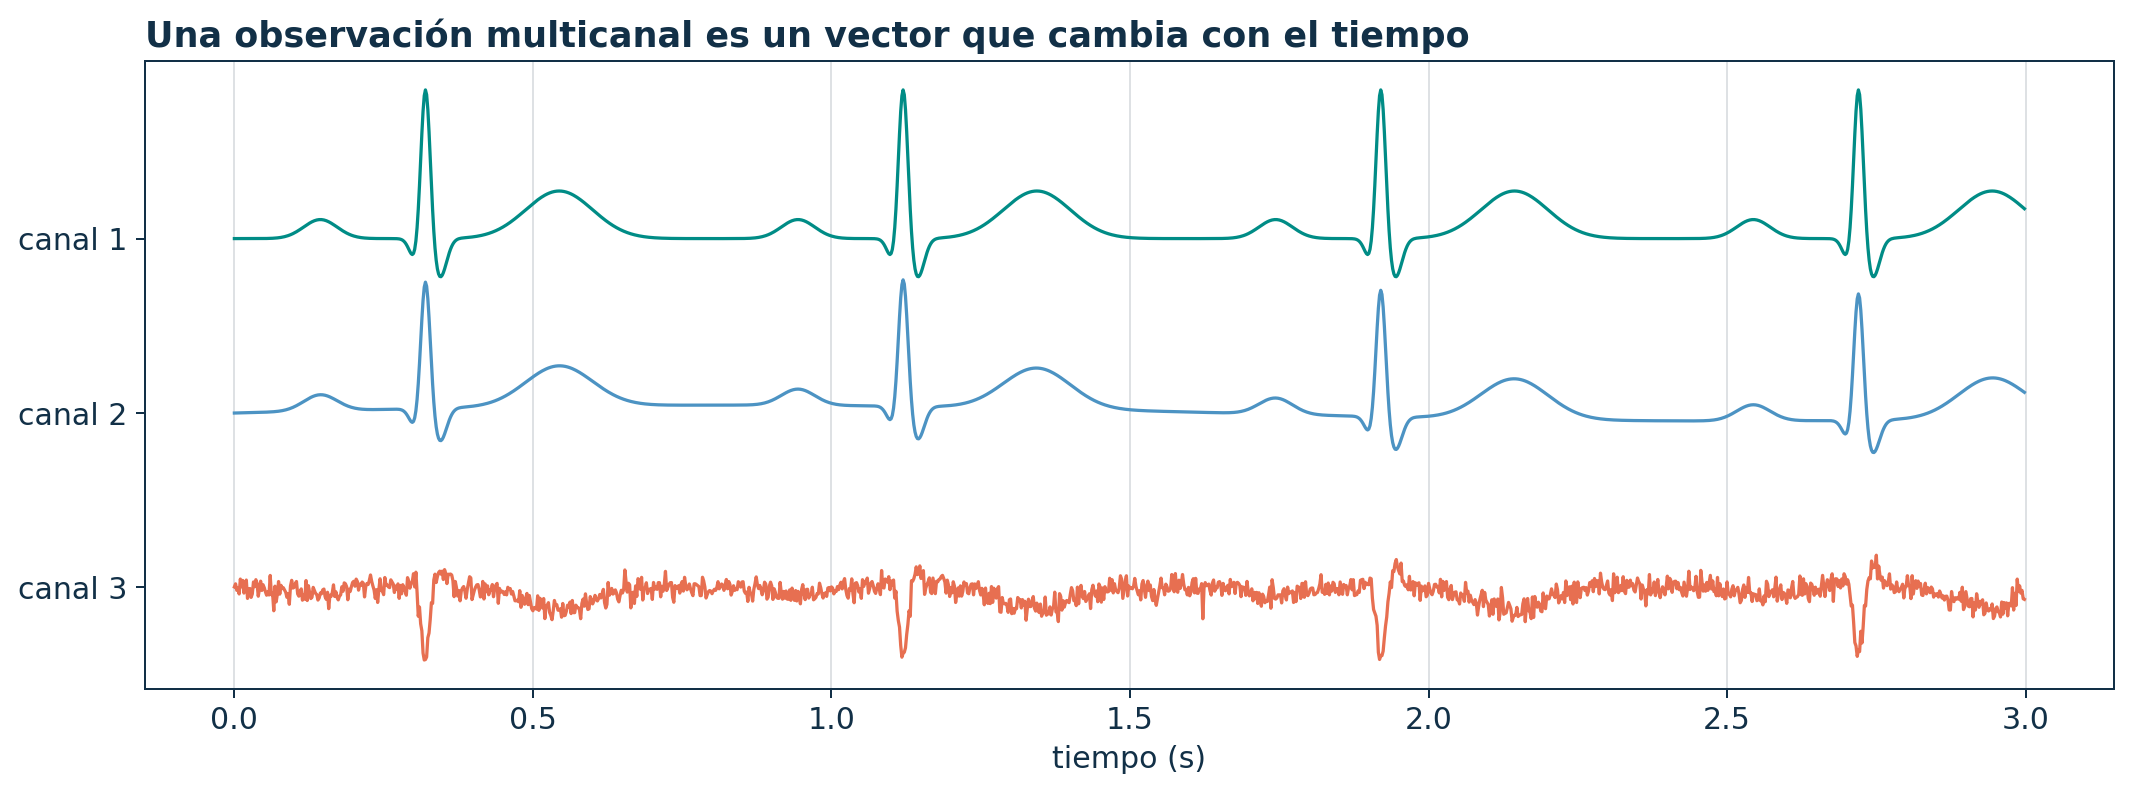
\includegraphics[width=0.85\linewidth,height=\textheight,keepaspectratio]{assets/04_multichannel.png}

\begin{tcolorbox}[enhanced jigsaw, arc=.35mm, bottomrule=.15mm, bottomtitle=1mm, breakable, colback=white, colbacktitle=quarto-callout-tip-color!10!white, colframe=quarto-callout-tip-color-frame, coltitle=black, left=2mm, leftrule=.75mm, opacityback=0, opacitybacktitle=0.6, rightrule=.15mm, title={Lectura}, titlerule=0mm, toprule=.15mm, toptitle=1mm]

Los canales pueden compartir una fuente, pero su amplitud y polaridad
dependen de la geometría, la referencia y la sensibilidad del sensor.

\end{tcolorbox}
\end{frame}

\begin{frame}[fragile,shrink]{Convenciones para arreglos multicanal}
\protect\phantomsection\label{convenciones-para-arreglos-multicanal}
Dos organizaciones comunes son:

\[
\mathbf{X}\in\mathbb{R}^{N\times M}
\quad\text{o}\quad
\mathbf{X}\in\mathbb{R}^{M\times N},
\]

donde \(N\) es el número de muestras y \(M\) el número de canales.

\begin{Shaded}
\begin{Highlighting}[]
\CommentTok{\# muestras por filas, canales por columnas}
\NormalTok{X }\OperatorTok{=}\NormalTok{ np.column\_stack([ecg\_I, ecg\_II, ecg\_III])}
\NormalTok{N, M }\OperatorTok{=}\NormalTok{ X.shape}

\CommentTok{\# seleccionar canal 2}
\NormalTok{x2 }\OperatorTok{=}\NormalTok{ X[:, }\DecValTok{1}\NormalTok{]}
\end{Highlighting}
\end{Shaded}

\begin{tcolorbox}[enhanced jigsaw, arc=.35mm, bottomrule=.15mm, bottomtitle=1mm, breakable, colback=white, colbacktitle=quarto-callout-important-color!10!white, colframe=quarto-callout-important-color-frame, coltitle=black, left=2mm, leftrule=.75mm, opacityback=0, opacitybacktitle=0.6, rightrule=.15mm, title={Regla práctica}, titlerule=0mm, toprule=.15mm, toptitle=1mm]

Documente la orientación del arreglo. Un error de ejes puede mezclar
operaciones temporales con operaciones entre canales.

\end{tcolorbox}
\end{frame}

\begin{frame}[fragile]{Actividad: audite un arreglo}
\protect\phantomsection\label{actividad-audite-un-arreglo}
Se recibe \texttt{X.shape\ ==\ (60000,\ 8)} y solo se informa que
corresponde a EEG.

\begin{enumerate}
\tightlist
\item
  Proponga dos interpretaciones posibles de los ejes.
\item
  Enumere cuatro metadatos indispensables.
\item
  Si \(f_s=250\) Hz y hay 60 000 muestras temporales, calcule la
  duración.
\item
  Explique por qué el número de canales no permite inferir el montaje.
\end{enumerate}

\begin{tcolorbox}[enhanced jigsaw, arc=.35mm, bottomrule=.15mm, bottomtitle=1mm, breakable, colback=white, colbacktitle=quarto-callout-note-color!10!white, colframe=quarto-callout-note-color-frame, coltitle=black, left=2mm, leftrule=.75mm, opacityback=0, opacitybacktitle=0.6, rightrule=.15mm, title={Respuesta parcial}, titlerule=0mm, toprule=.15mm, toptitle=1mm]

Si las 60 000 posiciones son muestras, la duración nominal es
\(60000/250=240\) s. La forma del arreglo por sí sola no identifica qué
eje corresponde al tiempo.

\end{tcolorbox}
\end{frame}

\begin{frame}{Cierre de la sesión 3}
\protect\phantomsection\label{cierre-de-la-sesiuxf3n-3}
\begin{tcolorbox}[enhanced jigsaw, arc=.35mm, bottomrule=.15mm, bottomtitle=1mm, breakable, colback=white, colbacktitle=quarto-callout-important-color!10!white, colframe=quarto-callout-important-color-frame, coltitle=black, left=2mm, leftrule=.75mm, opacityback=0, opacitybacktitle=0.6, rightrule=.15mm, title={Síntesis}, titlerule=0mm, toprule=.15mm, toptitle=1mm]

Una representación útil exige conocer el dominio, las unidades, la
frecuencia de muestreo y la organización de los canales. Python manipula
arreglos; el significado biomédico depende del contrato de datos.

\end{tcolorbox}

\textbf{Conexión:} una vez representada la señal, necesitamos medidas
que resuman su comportamiento sin perder de vista el intervalo
analizado.
\end{frame}

\section{Semana 2 · Sesión 2}\label{semana-2-sesiuxf3n-2}

\begin{frame}{Medir una señal es resumirla bajo un supuesto}
\protect\phantomsection\label{medir-una-seuxf1al-es-resumirla-bajo-un-supuesto}
Al finalizar esta sesión podrá:

\begin{itemize}
\tightlist
\item
  calcular medidas de localización, dispersión y magnitud;
\item
  diferenciar energía y potencia promedio;
\item
  interpretar RMS y amplitud pico a pico;
\item
  reconocer la dependencia respecto a la ventana;
\item
  evitar comparaciones inválidas entre registros.
\end{itemize}

\begin{tcolorbox}[enhanced jigsaw, arc=.35mm, bottomrule=.15mm, bottomtitle=1mm, breakable, colback=white, colbacktitle=quarto-callout-note-color!10!white, colframe=quarto-callout-note-color-frame, coltitle=black, left=2mm, leftrule=.75mm, opacityback=0, opacitybacktitle=0.6, rightrule=.15mm, title={Pregunta inicial}, titlerule=0mm, toprule=.15mm, toptitle=1mm]

¿Puede una sola cifra describir adecuadamente una señal con eventos
transitorios y oscilaciones sostenidas?

\end{tcolorbox}
\end{frame}

\begin{frame}{Media: nivel promedio con signo}
\protect\phantomsection\label{media-nivel-promedio-con-signo}
Para \(N\) muestras,

\[
\bar{x}=\frac{1}{N}\sum_{n=0}^{N-1}x[n].
\]

\begin{itemize}
\tightlist
\item
  Detecta desplazamientos del nivel basal.
\item
  Puede ser cercana a cero aunque la señal tenga amplitud elevada.
\item
  Es sensible a valores extremos.
\end{itemize}

\begin{tcolorbox}[enhanced jigsaw, arc=.35mm, bottomrule=.15mm, bottomtitle=1mm, breakable, colback=white, colbacktitle=quarto-callout-warning-color!10!white, colframe=quarto-callout-warning-color-frame, coltitle=black, left=2mm, leftrule=.75mm, opacityback=0, opacitybacktitle=0.6, rightrule=.15mm, title={Error frecuente}, titlerule=0mm, toprule=.15mm, toptitle=1mm]

Media cercana a cero no significa ``ausencia de señal''. Una oscilación
simétrica puede tener media cero y potencia distinta de cero.

\end{tcolorbox}
\end{frame}

\begin{frame}{Varianza y desviación estándar miden dispersión}
\protect\phantomsection\label{varianza-y-desviaciuxf3n-estuxe1ndar-miden-dispersiuxf3n}
Varianza poblacional:

\[
\sigma_x^2=\frac{1}{N}\sum_{n=0}^{N-1}\big(x[n]-\bar{x}\big)^2.
\]

Desviación estándar:

\[
\sigma_x=\sqrt{\sigma_x^2}.
\]

\begin{tcolorbox}[enhanced jigsaw, arc=.35mm, bottomrule=.15mm, bottomtitle=1mm, breakable, colback=white, colbacktitle=quarto-callout-note-color!10!white, colframe=quarto-callout-note-color-frame, coltitle=black, left=2mm, leftrule=.75mm, opacityback=0, opacitybacktitle=0.6, rightrule=.15mm, title={Interpretación}, titlerule=0mm, toprule=.15mm, toptitle=1mm]

La varianza tiene unidades al cuadrado; la desviación estándar conserva
las unidades de amplitud de la señal.

\end{tcolorbox}
\end{frame}

\begin{frame}{RMS cuantifica magnitud cuadrática}
\protect\phantomsection\label{rms-cuantifica-magnitud-cuadruxe1tica}
\[
x_{\mathrm{RMS}}
=\sqrt{\frac{1}{N}\sum_{n=0}^{N-1}x^2[n]}.
\]

\begin{itemize}
\tightlist
\item
  No cancela valores positivos y negativos.
\item
  Aumenta con componentes de gran amplitud.
\item
  Se relaciona con potencia promedio cuando la amplitud representa una
  magnitud física compatible.
\end{itemize}

\begin{tcolorbox}[enhanced jigsaw, arc=.35mm, bottomrule=.15mm, bottomtitle=1mm, breakable, colback=white, colbacktitle=quarto-callout-important-color!10!white, colframe=quarto-callout-important-color-frame, coltitle=black, left=2mm, leftrule=.75mm, opacityback=0, opacitybacktitle=0.6, rightrule=.15mm, title={Relación útil}, titlerule=0mm, toprule=.15mm, toptitle=1mm]

Si \(\bar{x}=0\), entonces \(x_{\mathrm{RMS}}=\sigma_x\). En general,
\(x_{\mathrm{RMS}}^2=\sigma_x^2+\bar{x}^2\).

\end{tcolorbox}
\end{frame}

\begin{frame}[shrink]{Media y RMS responden preguntas diferentes}
\protect\phantomsection\label{media-y-rms-responden-preguntas-diferentes}
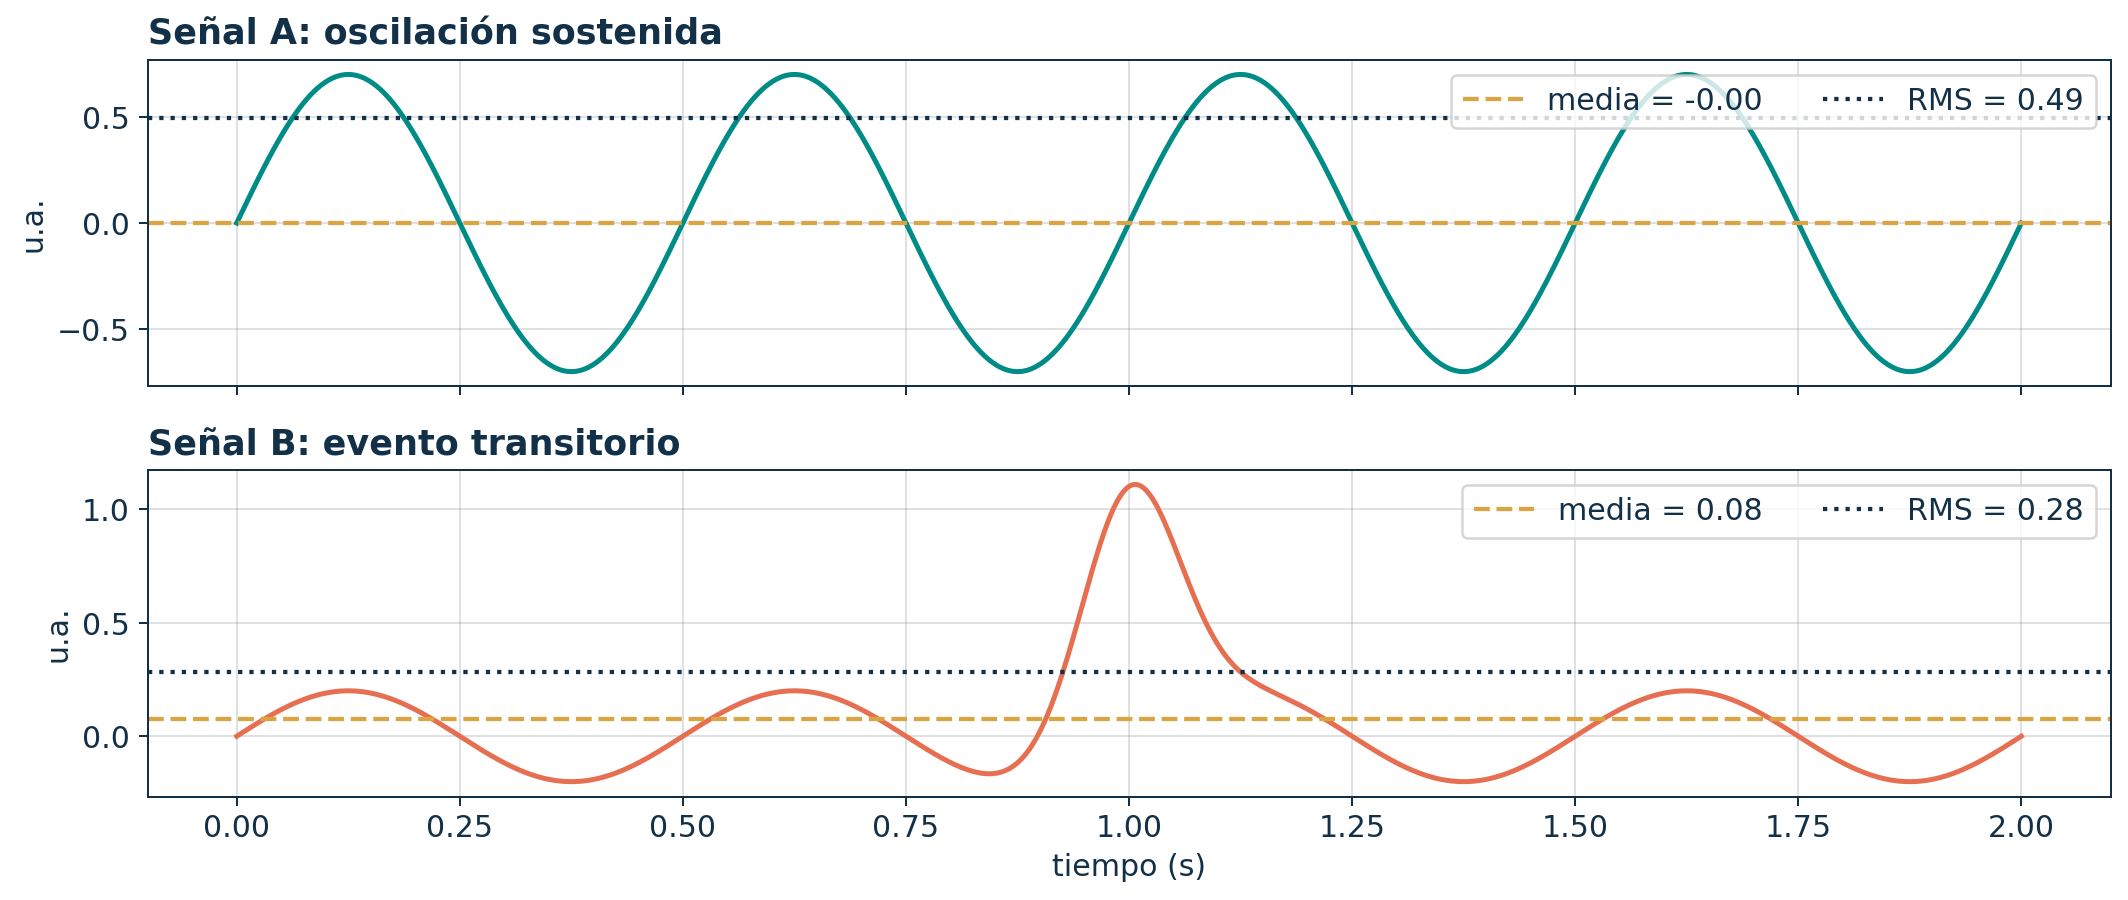
\includegraphics[width=0.84\linewidth,height=\textheight,keepaspectratio]{assets/05_temporal_measures.png}

\begin{tcolorbox}[enhanced jigsaw, arc=.35mm, bottomrule=.15mm, bottomtitle=1mm, breakable, colback=white, colbacktitle=quarto-callout-tip-color!10!white, colframe=quarto-callout-tip-color-frame, coltitle=black, left=2mm, leftrule=.75mm, opacityback=0, opacitybacktitle=0.6, rightrule=.15mm, title={Observe}, titlerule=0mm, toprule=.15mm, toptitle=1mm]

La señal oscilatoria presenta media casi nula y RMS apreciable. El
evento transitorio modifica tanto la media como el RMS, pero su efecto
depende de la duración del registro.

\end{tcolorbox}
\end{frame}

\begin{frame}[shrink]{Amplitud pico a pico y factor de cresta}
\protect\phantomsection\label{amplitud-pico-a-pico-y-factor-de-cresta}
Amplitud pico a pico:

\[x_{pp}=\max(x)-\min(x).\]

Factor de cresta:

\[C=\frac{\max |x[n]|}{x_{\mathrm{RMS}}}.\]

\begin{tcolorbox}[enhanced jigsaw, arc=.35mm, bottomrule=.15mm, bottomtitle=1mm, breakable, colback=white, colbacktitle=quarto-callout-note-color!10!white, colframe=quarto-callout-note-color-frame, coltitle=black, left=2mm, leftrule=.75mm, opacityback=0, opacitybacktitle=0.6, rightrule=.15mm, title={Lectura}, titlerule=0mm, toprule=.15mm, toptitle=1mm]

\(x_{pp}\) describe el rango observado; el factor de cresta contrasta el
máximo con la magnitud típica y ayuda a señalar eventos impulsivos.

\end{tcolorbox}

\begin{tcolorbox}[enhanced jigsaw, arc=.35mm, bottomrule=.15mm, bottomtitle=1mm, breakable, colback=white, colbacktitle=quarto-callout-warning-color!10!white, colframe=quarto-callout-warning-color-frame, coltitle=black, left=2mm, leftrule=.75mm, opacityback=0, opacitybacktitle=0.6, rightrule=.15mm, title={Limitación}, titlerule=0mm, toprule=.15mm, toptitle=1mm]

Ambas medidas son sensibles a artefactos y valores extremos. No deben
interpretarse sin inspección y control de calidad.

\end{tcolorbox}
\end{frame}

\begin{frame}{Energía y potencia promedio}
\protect\phantomsection\label{energuxeda-y-potencia-promedio}
Para una secuencia de energía:

\[
E_x=\sum_{n=-\infty}^{\infty}|x[n]|^2.
\]

Para una señal persistente, la potencia promedio se define como

\[
P_x=\lim_{N\to\infty}\frac{1}{2N+1}
\sum_{n=-N}^{N}|x[n]|^2.
\]

\begin{tcolorbox}[enhanced jigsaw, arc=.35mm, bottomrule=.15mm, bottomtitle=1mm, breakable, colback=white, colbacktitle=quarto-callout-important-color!10!white, colframe=quarto-callout-important-color-frame, coltitle=black, left=2mm, leftrule=.75mm, opacityback=0, opacitybacktitle=0.6, rightrule=.15mm, title={Distinción}, titlerule=0mm, toprule=.15mm, toptitle=1mm]

Una señal transitoria puede tener energía finita y potencia promedio
nula; una señal periódica no nula suele tener energía infinita y
potencia promedio finita.

\end{tcolorbox}
\end{frame}

\begin{frame}{La duración de análisis modifica el resultado}
\protect\phantomsection\label{la-duraciuxf3n-de-anuxe1lisis-modifica-el-resultado}
Suponga un evento de energía fija dentro de ventanas cada vez más
largas:

\begin{itemize}
\tightlist
\item
  la energía acumulada puede permanecer aproximadamente estable;
\item
  el valor RMS disminuye al incluir más muestras sin actividad;
\item
  la media y la varianza cambian con la proporción entre evento y
  reposo.
\end{itemize}

\begin{tcolorbox}[enhanced jigsaw, arc=.35mm, bottomrule=.15mm, bottomtitle=1mm, breakable, colback=white, colbacktitle=quarto-callout-caution-color!10!white, colframe=quarto-callout-caution-color-frame, coltitle=black, left=2mm, leftrule=.75mm, opacityback=0, opacitybacktitle=0.6, rightrule=.15mm, title={Consecuencia metodológica}, titlerule=0mm, toprule=.15mm, toptitle=1mm]

Comparar RMS, media o varianza exige usar ventanas equivalentes y
justificar su relación con el fenómeno fisiológico.

\end{tcolorbox}
\end{frame}

\begin{frame}[shrink]{El RMS móvil revela variación temporal}
\protect\phantomsection\label{el-rms-muxf3vil-revela-variaciuxf3n-temporal}
Para una ventana de \(L\) muestras:

\[
x_{\mathrm{RMS}}[n]
=\sqrt{\frac{1}{L}\sum_{k=0}^{L-1}x^2[n-k]}.
\]

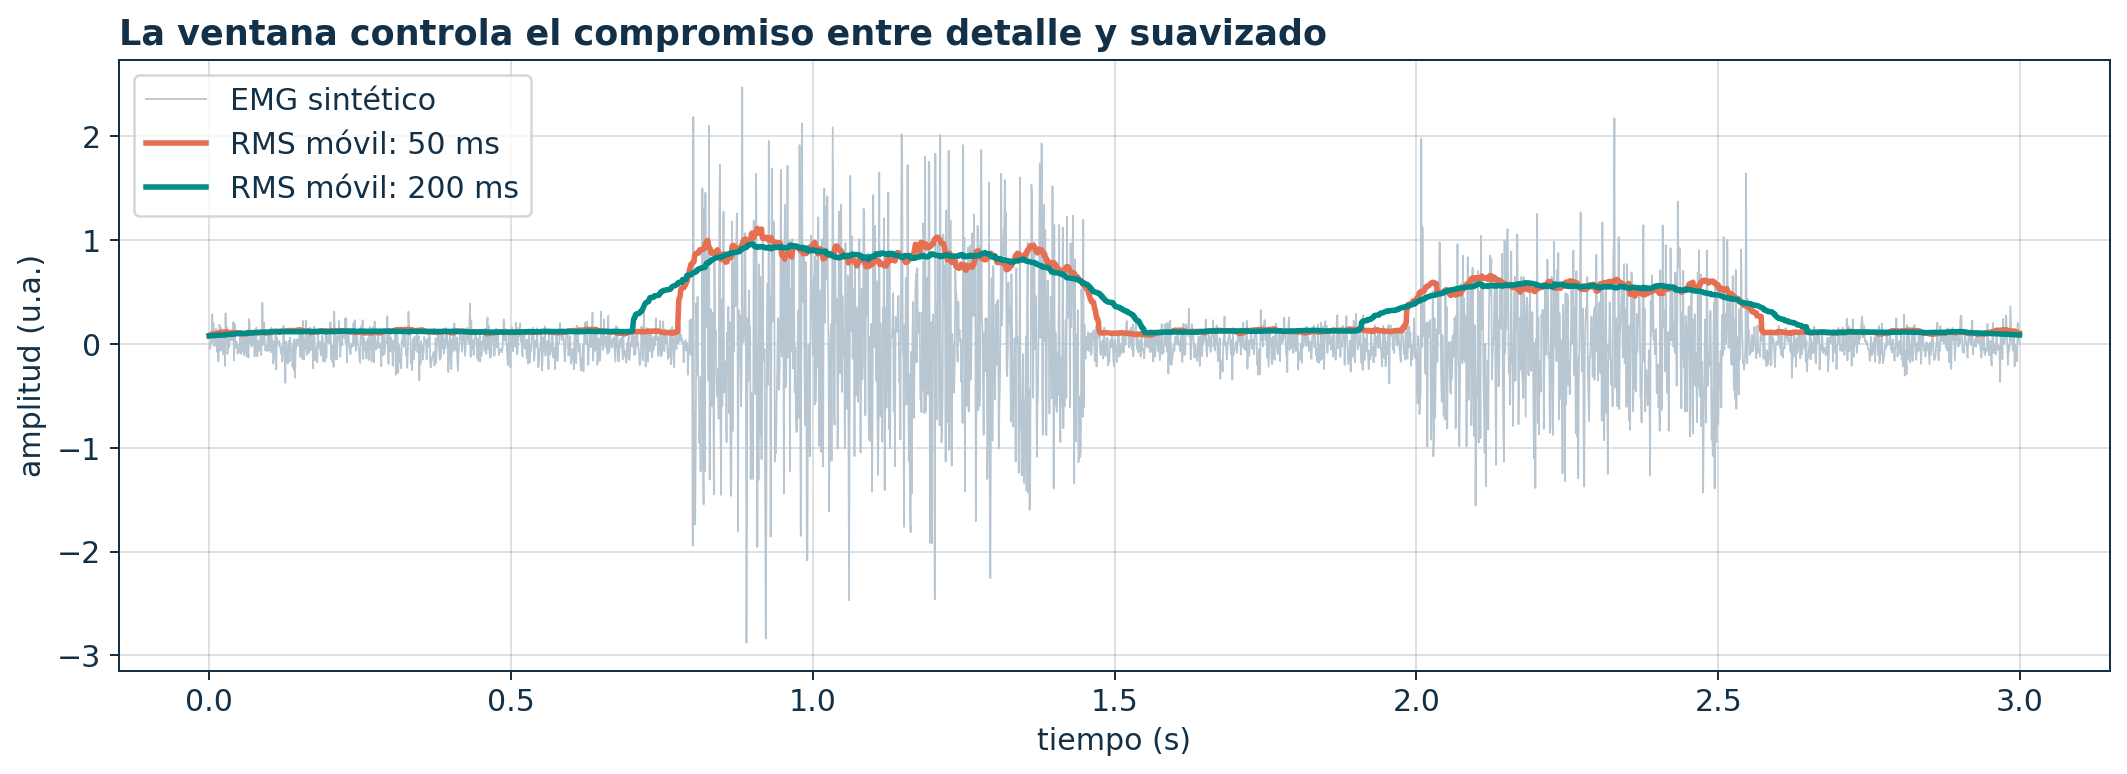
\includegraphics[width=0.8\linewidth,height=\textheight,keepaspectratio]{assets/06_rms_windows.png}

\begin{tcolorbox}[enhanced jigsaw, arc=.35mm, bottomrule=.15mm, bottomtitle=1mm, breakable, colback=white, colbacktitle=quarto-callout-note-color!10!white, colframe=quarto-callout-note-color-frame, coltitle=black, left=2mm, leftrule=.75mm, opacityback=0, opacitybacktitle=0.6, rightrule=.15mm, title={Compromiso}, titlerule=0mm, toprule=.15mm, toptitle=1mm]

Una ventana corta sigue cambios rápidos, pero fluctúa más. Una ventana
larga suaviza, pero reduce la precisión temporal.

\end{tcolorbox}
\end{frame}

\begin{frame}[fragile,shrink]{Cálculo reproducible en Python}
\protect\phantomsection\label{cuxe1lculo-reproducible-en-python}
\begin{Shaded}
\begin{Highlighting}[]
\ImportTok{import}\NormalTok{ numpy }\ImportTok{as}\NormalTok{ np}

\KeywordTok{def}\NormalTok{ temporal\_features(x):}
\NormalTok{    x }\OperatorTok{=}\NormalTok{ np.asarray(x, dtype}\OperatorTok{=}\BuiltInTok{float}\NormalTok{)}
    \ControlFlowTok{return}\NormalTok{ \{}
        \StringTok{"mean"}\NormalTok{: np.mean(x),}
        \StringTok{"std"}\NormalTok{: np.std(x, ddof}\OperatorTok{=}\DecValTok{0}\NormalTok{),}
        \StringTok{"rms"}\NormalTok{: np.sqrt(np.mean(x}\OperatorTok{**}\DecValTok{2}\NormalTok{)),}
        \StringTok{"peak\_to\_peak"}\NormalTok{: np.ptp(x),}
        \StringTok{"energy"}\NormalTok{: np.}\BuiltInTok{sum}\NormalTok{(x}\OperatorTok{**}\DecValTok{2}\NormalTok{),}
\NormalTok{    \}}
\end{Highlighting}
\end{Shaded}

\begin{tcolorbox}[enhanced jigsaw, arc=.35mm, bottomrule=.15mm, bottomtitle=1mm, breakable, colback=white, colbacktitle=quarto-callout-tip-color!10!white, colframe=quarto-callout-tip-color-frame, coltitle=black, left=2mm, leftrule=.75mm, opacityback=0, opacitybacktitle=0.6, rightrule=.15mm, title={Buena práctica}, titlerule=0mm, toprule=.15mm, toptitle=1mm]

La función calcula números; el reporte debe añadir unidades, ventana,
preprocesamiento y significado fisiológico.

\end{tcolorbox}
\end{frame}

\begin{frame}{Antes de comparar dos registros}
\protect\phantomsection\label{antes-de-comparar-dos-registros}
Verifique:

\begin{enumerate}
\tightlist
\item
  misma unidad y factor de escala;
\item
  misma duración o estrategia de segmentación;
\item
  mismo ancho de banda y referencia;
\item
  ausencia de saturación;
\item
  proporción comparable de actividad y reposo;
\item
  tratamiento consistente de artefactos;
\item
  métrica vinculada con la pregunta.
\end{enumerate}

\begin{tcolorbox}[enhanced jigsaw, arc=.35mm, bottomrule=.15mm, bottomtitle=1mm, breakable, colback=white, colbacktitle=quarto-callout-important-color!10!white, colframe=quarto-callout-important-color-frame, coltitle=black, left=2mm, leftrule=.75mm, opacityback=0, opacitybacktitle=0.6, rightrule=.15mm, title={Principio de comparabilidad}, titlerule=0mm, toprule=.15mm, toptitle=1mm]

Dos números solo son comparables cuando proceden de definiciones y
condiciones equivalentes.

\end{tcolorbox}
\end{frame}

\begin{frame}{Actividad: elija una métrica defendible}
\protect\phantomsection\label{actividad-elija-una-muxe9trica-defendible}
Para cada objetivo, seleccione una métrica inicial y señale una
limitación:

\begin{itemize}
\tightlist
\item
  detectar desplazamiento de línea base;
\item
  cuantificar magnitud de una contracción EMG;
\item
  describir un evento extremo;
\item
  comparar dispersión entre segmentos;
\item
  resumir una oscilación periódica.
\end{itemize}

\begin{tcolorbox}[enhanced jigsaw, arc=.35mm, bottomrule=.15mm, bottomtitle=1mm, breakable, colback=white, colbacktitle=quarto-callout-tip-color!10!white, colframe=quarto-callout-tip-color-frame, coltitle=black, left=2mm, leftrule=.75mm, opacityback=0, opacitybacktitle=0.6, rightrule=.15mm, title={No existe una respuesta universal}, titlerule=0mm, toprule=.15mm, toptitle=1mm]

La selección se evalúa por la coherencia entre objetivo, definición
matemática y comportamiento esperado de la señal.

\end{tcolorbox}
\end{frame}

\begin{frame}{Cierre de la semana 2}
\protect\phantomsection\label{cierre-de-la-semana-2}
\begin{tcolorbox}[enhanced jigsaw, arc=.35mm, bottomrule=.15mm, bottomtitle=1mm, breakable, colback=white, colbacktitle=quarto-callout-important-color!10!white, colframe=quarto-callout-important-color-frame, coltitle=black, left=2mm, leftrule=.75mm, opacityback=0, opacitybacktitle=0.6, rightrule=.15mm, title={Síntesis}, titlerule=0mm, toprule=.15mm, toptitle=1mm]

Las métricas temporales son resúmenes dependientes de la ventana. Media,
desviación, RMS, energía y amplitud pico a pico describen propiedades
diferentes; ninguna reemplaza la inspección ni el contexto biomédico.

\end{tcolorbox}

\textbf{Preparación para la semana 3:} repase trigonometría, radianes,
frecuencia, periodo y operaciones sobre funciones.
\end{frame}

\section{Semana 3 · Sesión 1}\label{semana-3-sesiuxf3n-1}

\begin{frame}{La sinusoide es un bloque fundamental}
\protect\phantomsection\label{la-sinusoide-es-un-bloque-fundamental}
Al finalizar esta sesión podrá:

\begin{itemize}
\tightlist
\item
  interpretar amplitud, periodo, frecuencia y fase;
\item
  convertir entre frecuencia ordinaria y angular;
\item
  establecer periodicidad en tiempo continuo y discreto;
\item
  determinar cuándo la suma de señales periódicas también es periódica;
\item
  generar sinusoides correctamente en Python.
\end{itemize}

\begin{tcolorbox}[enhanced jigsaw, arc=.35mm, bottomrule=.15mm, bottomtitle=1mm, breakable, colback=white, colbacktitle=quarto-callout-note-color!10!white, colframe=quarto-callout-note-color-frame, coltitle=black, left=2mm, leftrule=.75mm, opacityback=0, opacitybacktitle=0.6, rightrule=.15mm, title={Pregunta inicial}, titlerule=0mm, toprule=.15mm, toptitle=1mm]

¿Dos sinusoides con la misma frecuencia, pero diferente fase, contienen
la misma información temporal?

\end{tcolorbox}
\end{frame}

\begin{frame}{Modelo de una sinusoide continua}
\protect\phantomsection\label{modelo-de-una-sinusoide-continua}
\[
x(t)=A\cos(2\pi f_0t+\phi)
=A\cos(\omega_0t+\phi).
\]

{\def\LTcaptype{none} % do not increment counter
\begin{longtable}[]{@{}lll@{}}
\toprule\noalign{}
Parámetro & Significado & Unidad \\
\midrule\noalign{}
\endhead
\(A\) & amplitud máxima respecto al nivel cero & unidad de \(x\) \\
\(f_0\) & ciclos por segundo & Hz \\
\(T_0\) & duración de un ciclo & s \\
\(\omega_0\) & frecuencia angular & rad/s \\
\(\phi\) & desplazamiento angular inicial & rad \\
\bottomrule\noalign{}
\end{longtable}
}

\begin{tcolorbox}[enhanced jigsaw, arc=.35mm, bottomrule=.15mm, bottomtitle=1mm, breakable, colback=white, colbacktitle=quarto-callout-important-color!10!white, colframe=quarto-callout-important-color-frame, coltitle=black, left=2mm, leftrule=.75mm, opacityback=0, opacitybacktitle=0.6, rightrule=.15mm, title={Relaciones esenciales}, titlerule=0mm, toprule=.15mm, toptitle=1mm]

\(T_0=1/f_0\) y \(\omega_0=2\pi f_0\).

\end{tcolorbox}
\end{frame}

\begin{frame}[shrink]{Lea cada parámetro en la forma de onda}
\protect\phantomsection\label{lea-cada-paruxe1metro-en-la-forma-de-onda}
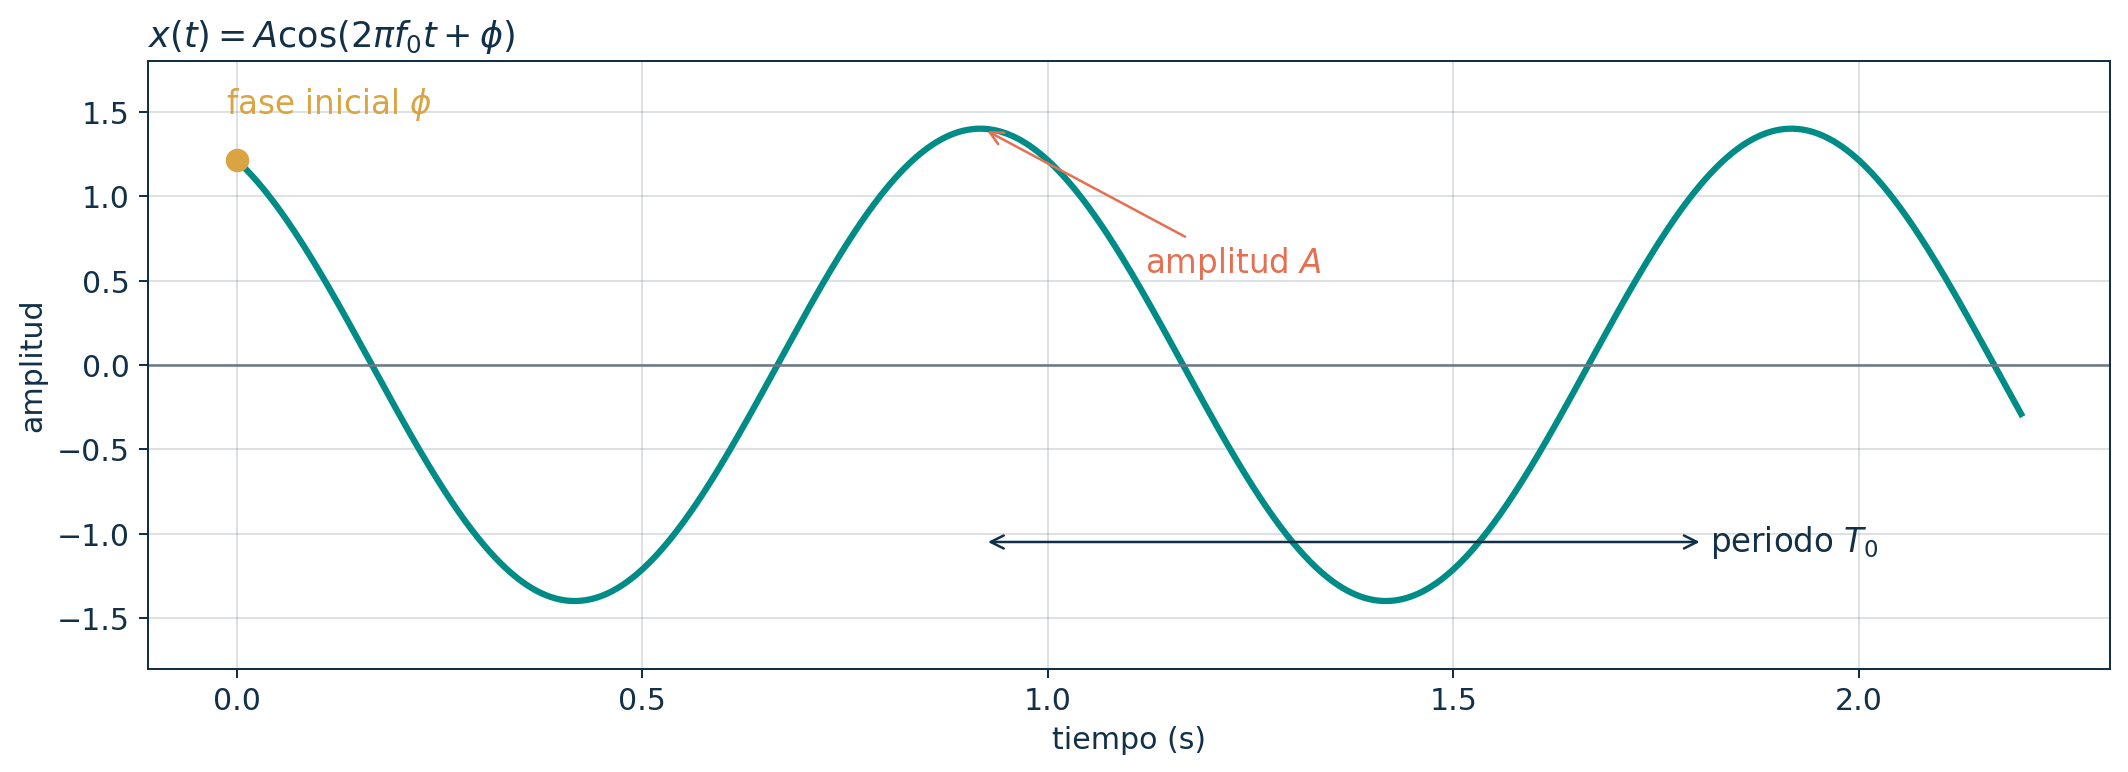
\includegraphics[width=0.84\linewidth,height=\textheight,keepaspectratio]{assets/07_sinusoid_parameters.png}

\begin{tcolorbox}[enhanced jigsaw, arc=.35mm, bottomrule=.15mm, bottomtitle=1mm, breakable, colback=white, colbacktitle=quarto-callout-note-color!10!white, colframe=quarto-callout-note-color-frame, coltitle=black, left=2mm, leftrule=.75mm, opacityback=0, opacitybacktitle=0.6, rightrule=.15mm, title={Interpretación}, titlerule=0mm, toprule=.15mm, toptitle=1mm]

La amplitud escala verticalmente; el periodo controla la repetición
horizontal; la fase modifica la posición del ciclo respecto al origen.

\end{tcolorbox}
\end{frame}

\begin{frame}{Frecuencia no es rapidez de propagación}
\protect\phantomsection\label{frecuencia-no-es-rapidez-de-propagaciuxf3n}
\begin{itemize}
\tightlist
\item
  \textbf{Frecuencia:} número de ciclos por unidad de tiempo.
\item
  \textbf{Periodo:} duración de un ciclo.
\item
  \textbf{Fase:} posición dentro del ciclo.
\item
  \textbf{Velocidad de propagación:} rapidez con la que una perturbación
  se desplaza en el espacio.
\end{itemize}

\begin{tcolorbox}[enhanced jigsaw, arc=.35mm, bottomrule=.15mm, bottomtitle=1mm, breakable, colback=white, colbacktitle=quarto-callout-warning-color!10!white, colframe=quarto-callout-warning-color-frame, coltitle=black, left=2mm, leftrule=.75mm, opacityback=0, opacitybacktitle=0.6, rightrule=.15mm, title={Error conceptual}, titlerule=0mm, toprule=.15mm, toptitle=1mm]

Una oscilación de mayor frecuencia repite ciclos más rápidamente, pero
ello no implica que se propague más rápido por un tejido.

\end{tcolorbox}
\end{frame}

\begin{frame}[shrink]{La fase expresa alineación temporal relativa}
\protect\phantomsection\label{la-fase-expresa-alineaciuxf3n-temporal-relativa}
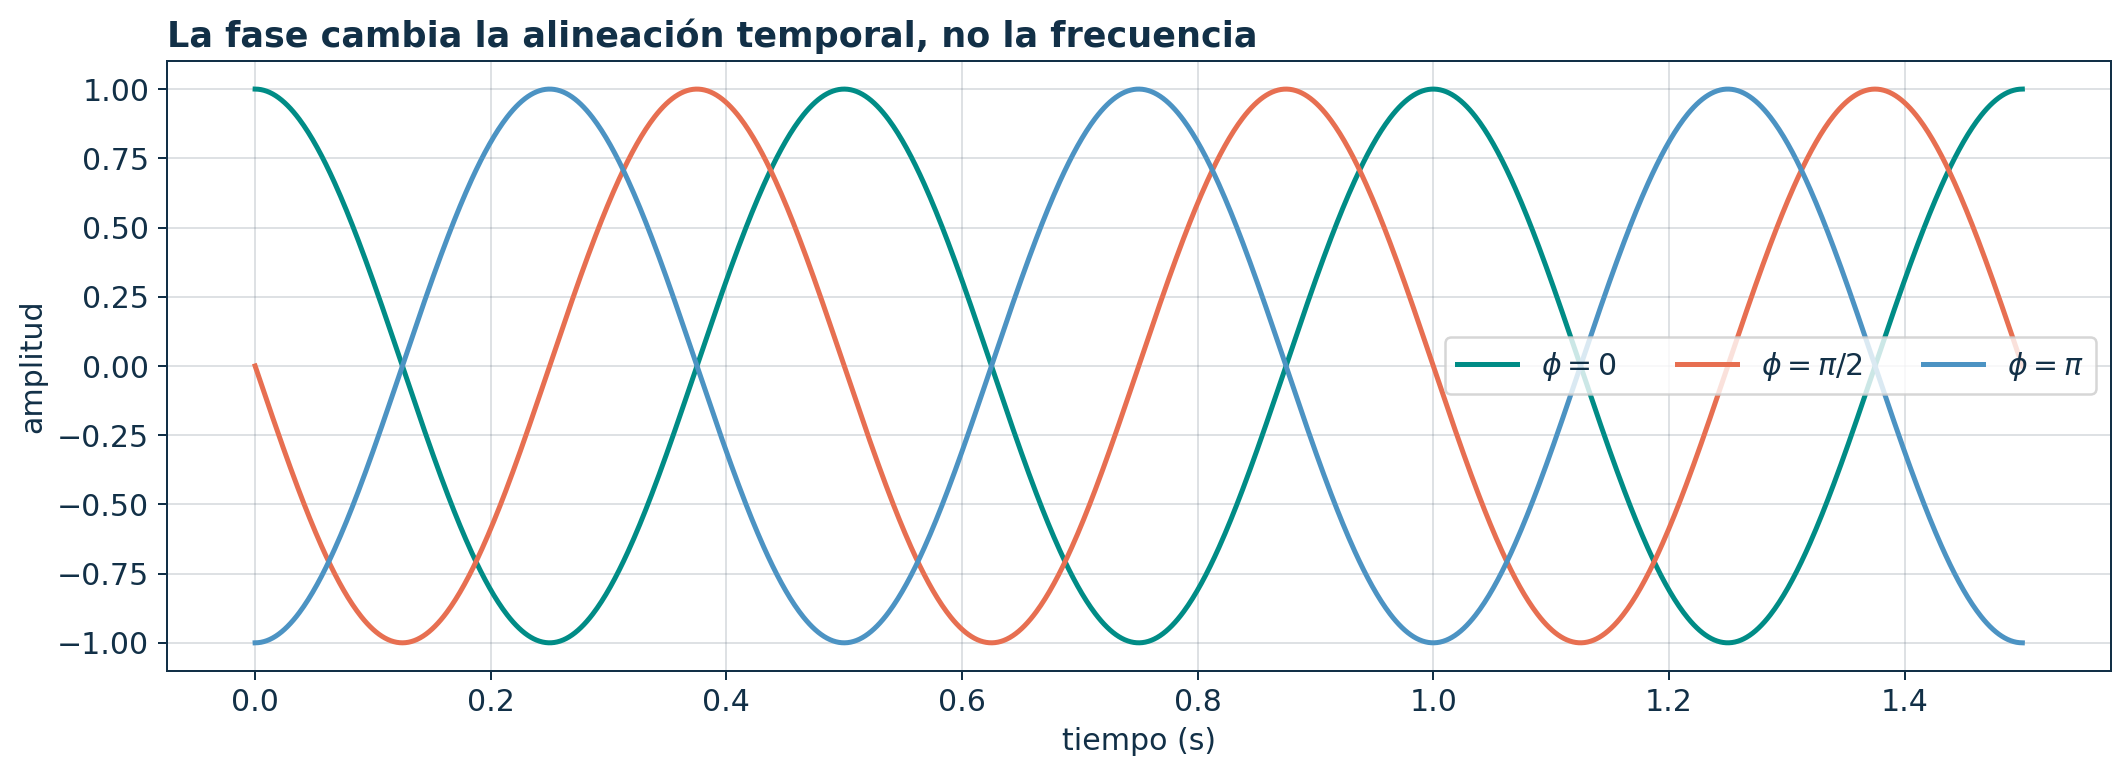
\includegraphics[width=0.83\linewidth,height=\textheight,keepaspectratio]{assets/08_phase_comparison.png}

Para una frecuencia fija, una fase \(\phi\) equivale a un desplazamiento
temporal

\[
t_0=-\frac{\phi}{\omega_0},
\]

según la convención \(x(t)=A\cos(\omega_0t+\phi)\).
\end{frame}

\begin{frame}{Periodicidad en tiempo continuo}
\protect\phantomsection\label{periodicidad-en-tiempo-continuo}
Una señal es periódica si existe \(T>0\) tal que

\[x(t+T)=x(t)\quad\text{para todo }t.\]

El menor valor positivo que satisface la condición se denomina
\textbf{periodo fundamental} \(T_0\).

\begin{tcolorbox}[enhanced jigsaw, arc=.35mm, bottomrule=.15mm, bottomtitle=1mm, breakable, colback=white, colbacktitle=quarto-callout-warning-color!10!white, colframe=quarto-callout-warning-color-frame, coltitle=black, left=2mm, leftrule=.75mm, opacityback=0, opacitybacktitle=0.6, rightrule=.15mm, title={Precisión matemática}, titlerule=0mm, toprule=.15mm, toptitle=1mm]

No todo valor que satisface la igualdad es fundamental. Si \(T_0\) es
fundamental, \(2T_0\), \(3T_0\), \ldots{} también son periodos.

\end{tcolorbox}
\end{frame}

\begin{frame}[shrink]{Periodicidad en tiempo discreto}
\protect\phantomsection\label{periodicidad-en-tiempo-discreto}
Una secuencia es periódica si existe un entero \(N>0\) tal que

\[x[n+N]=x[n]\quad\text{para todo }n.\]

Para

\[x[n]=A\cos(\Omega_0n+\phi),\]

la secuencia es periódica si y solo si

\[\frac{\Omega_0}{2\pi}\in\mathbb{Q}.\]

\begin{tcolorbox}[enhanced jigsaw, arc=.35mm, bottomrule=.15mm, bottomtitle=1mm, breakable, colback=white, colbacktitle=quarto-callout-important-color!10!white, colframe=quarto-callout-important-color-frame, coltitle=black, left=2mm, leftrule=.75mm, opacityback=0, opacitybacktitle=0.6, rightrule=.15mm, title={Diferencia clave}, titlerule=0mm, toprule=.15mm, toptitle=1mm]

Toda sinusoide continua es periódica. Una sinusoide discreta no
necesariamente lo es.

\end{tcolorbox}
\end{frame}

\begin{frame}{Ejemplo de periodicidad discreta}
\protect\phantomsection\label{ejemplo-de-periodicidad-discreta}
Considere

\[x[n]=\cos\left(\frac{3\pi}{5}n\right).\]

Buscamos enteros \(N,k>0\) tales que

\[\frac{3\pi}{5}N=2\pi k
\quad\Longrightarrow\quad 3N=10k.\]

El menor \(N\) que satisface la igualdad es \(N_0=10\).

\begin{tcolorbox}[enhanced jigsaw, arc=.35mm, bottomrule=.15mm, bottomtitle=1mm, breakable, colback=white, colbacktitle=quarto-callout-tip-color!10!white, colframe=quarto-callout-tip-color-frame, coltitle=black, left=2mm, leftrule=.75mm, opacityback=0, opacitybacktitle=0.6, rightrule=.15mm, title={Procedimiento}, titlerule=0mm, toprule=.15mm, toptitle=1mm]

Iguale \(\Omega_0N\) con un múltiplo entero de \(2\pi\) y encuentre el
menor \(N\) positivo.

\end{tcolorbox}
\end{frame}

\begin{frame}{¿Cuándo es periódica la suma?}
\protect\phantomsection\label{cuuxe1ndo-es-periuxf3dica-la-suma}
Si \(x_1(t)\) y \(x_2(t)\) tienen periodos fundamentales \(T_1\) y
\(T_2\), la suma será periódica cuando

\[
\frac{T_1}{T_2}\in\mathbb{Q}.
\]

El periodo común es un múltiplo simultáneo de \(T_1\) y \(T_2\).

\begin{tcolorbox}[enhanced jigsaw, arc=.35mm, bottomrule=.15mm, bottomtitle=1mm, breakable, colback=white, colbacktitle=quarto-callout-note-color!10!white, colframe=quarto-callout-note-color-frame, coltitle=black, left=2mm, leftrule=.75mm, opacityback=0, opacitybacktitle=0.6, rightrule=.15mm, title={Lectura}, titlerule=0mm, toprule=.15mm, toptitle=1mm]

La existencia de un periodo común exige que los ciclos puedan volver a
alinearse exactamente.

\end{tcolorbox}
\end{frame}

\begin{frame}[shrink]{Dos periodos conmensurables vuelven a alinearse}
\protect\phantomsection\label{dos-periodos-conmensurables-vuelven-a-alinearse}
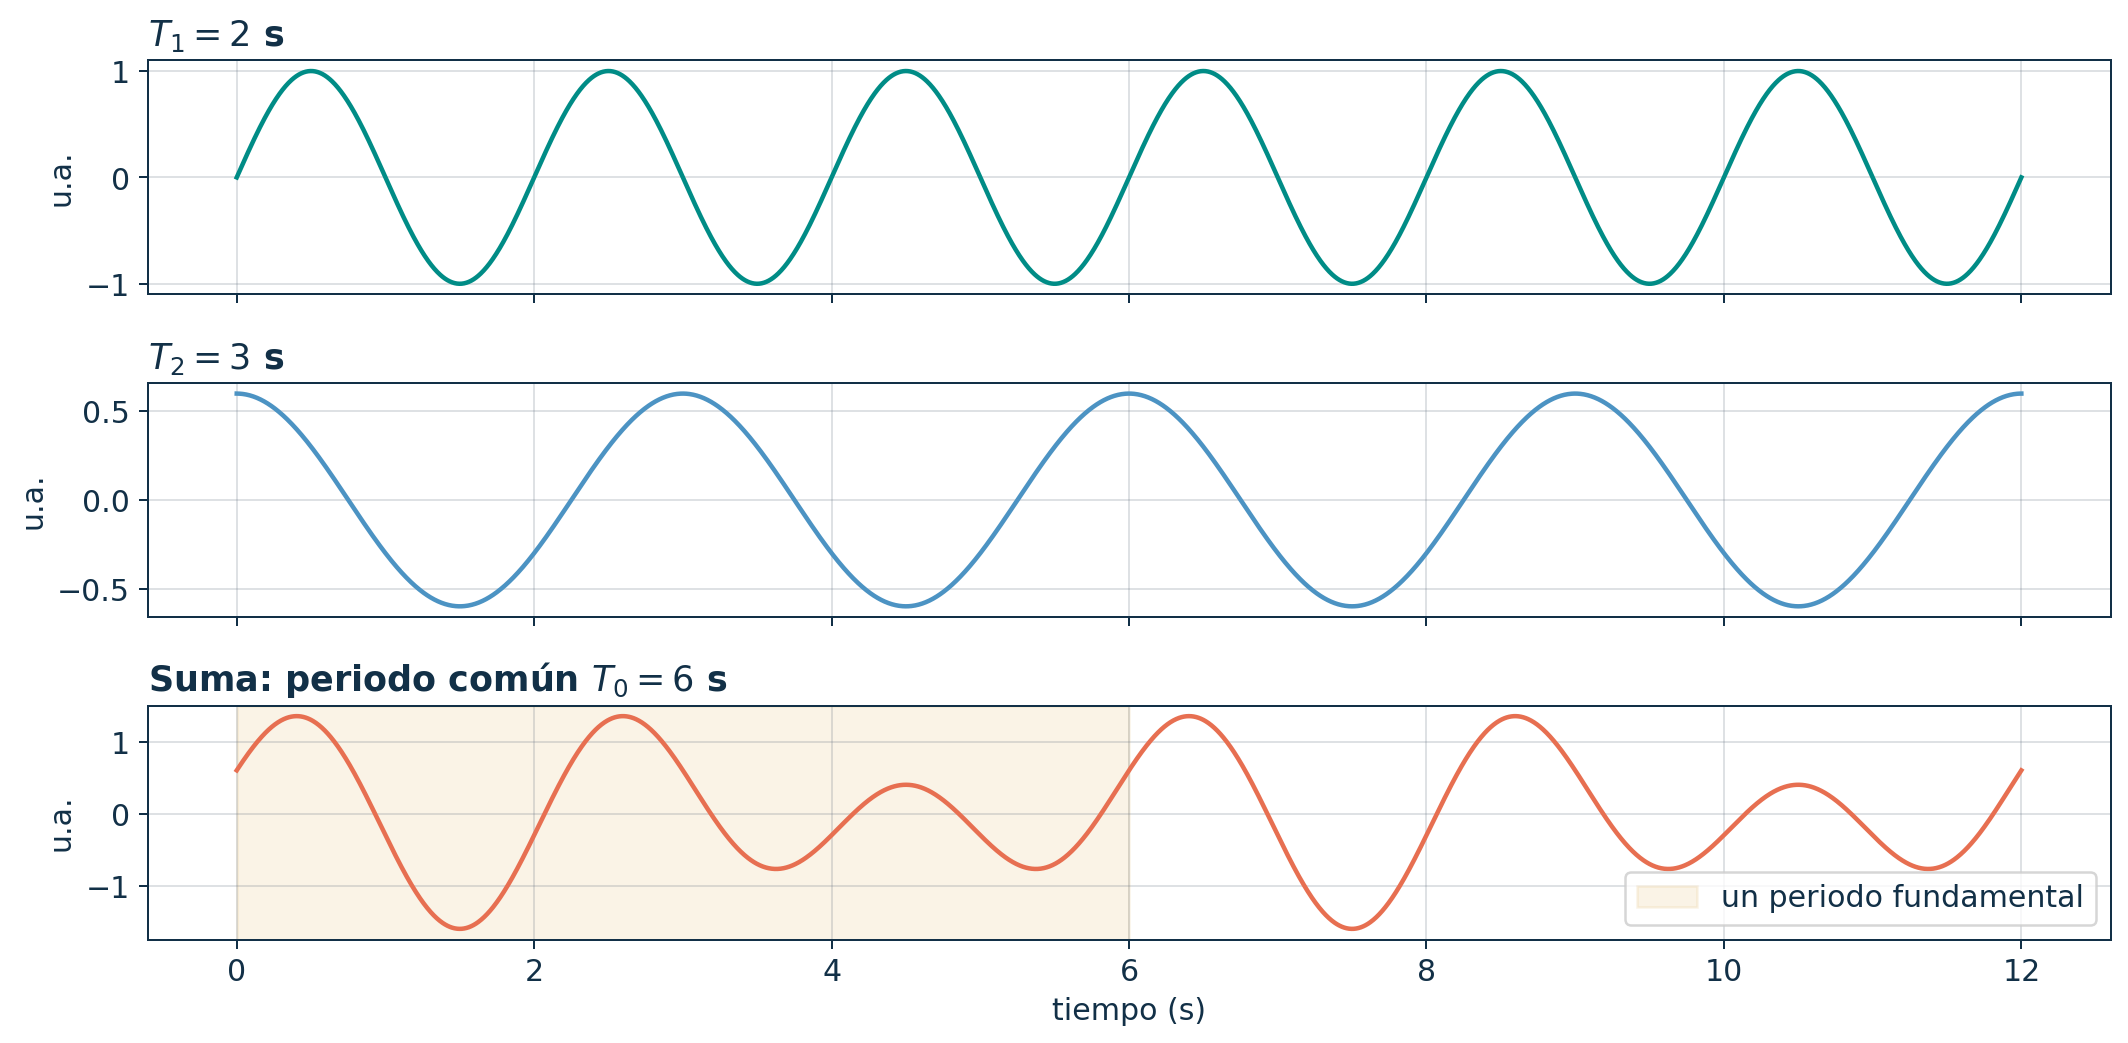
\includegraphics[width=0.8\linewidth,height=\textheight,keepaspectratio]{assets/09_periodic_sum.png}

\begin{tcolorbox}[enhanced jigsaw, arc=.35mm, bottomrule=.15mm, bottomtitle=1mm, breakable, colback=white, colbacktitle=quarto-callout-important-color!10!white, colframe=quarto-callout-important-color-frame, coltitle=black, left=2mm, leftrule=.75mm, opacityback=0, opacitybacktitle=0.6, rightrule=.15mm, title={Resultado}, titlerule=0mm, toprule=.15mm, toptitle=1mm]

Para \(T_1=2\) s y \(T_2=3\) s, el menor periodo común es \(T_0=6\) s.

\end{tcolorbox}
\end{frame}

\begin{frame}{Las bioseñales no suelen ser perfectamente periódicas}
\protect\phantomsection\label{las-bioseuxf1ales-no-suelen-ser-perfectamente-periuxf3dicas}
En fisiología es común observar:

\begin{itemize}
\tightlist
\item
  \textbf{cuasiperiodicidad:} ciclos similares, pero no idénticos;
\item
  \textbf{variabilidad:} duración o amplitud cambiante;
\item
  \textbf{transitorios:} eventos que aparecen y desaparecen;
\item
  \textbf{modulación:} una oscilación cambia con otra escala temporal;
\item
  \textbf{no estacionariedad:} las propiedades estadísticas evolucionan.
\end{itemize}

\begin{tcolorbox}[enhanced jigsaw, arc=.35mm, bottomrule=.15mm, bottomtitle=1mm, breakable, colback=white, colbacktitle=quarto-callout-caution-color!10!white, colframe=quarto-callout-caution-color-frame, coltitle=black, left=2mm, leftrule=.75mm, opacityback=0, opacitybacktitle=0.6, rightrule=.15mm, title={Interpretación biomédica}, titlerule=0mm, toprule=.15mm, toptitle=1mm]

Llamar ``periódico'' a un ECG o una señal respiratoria real suele ser
una aproximación local, no una identidad matemática exacta.

\end{tcolorbox}
\end{frame}

\begin{frame}[fragile,shrink]{Generación de sinusoides en Python}
\protect\phantomsection\label{generaciuxf3n-de-sinusoides-en-python}
\begin{Shaded}
\begin{Highlighting}[]
\ImportTok{import}\NormalTok{ numpy }\ImportTok{as}\NormalTok{ np}
\ImportTok{import}\NormalTok{ matplotlib.pyplot }\ImportTok{as}\NormalTok{ plt}

\NormalTok{fs }\OperatorTok{=} \DecValTok{500}
\NormalTok{t }\OperatorTok{=}\NormalTok{ np.arange(}\DecValTok{0}\NormalTok{, }\DecValTok{2}\NormalTok{, }\DecValTok{1}\OperatorTok{/}\NormalTok{fs)}

\NormalTok{A }\OperatorTok{=} \FloatTok{1.2}
\NormalTok{f0 }\OperatorTok{=} \DecValTok{8}
\NormalTok{phi }\OperatorTok{=}\NormalTok{ np.pi }\OperatorTok{/} \DecValTok{4}
\NormalTok{x }\OperatorTok{=}\NormalTok{ A }\OperatorTok{*}\NormalTok{ np.cos(}\DecValTok{2}\OperatorTok{*}\NormalTok{np.pi}\OperatorTok{*}\NormalTok{f0}\OperatorTok{*}\NormalTok{t }\OperatorTok{+}\NormalTok{ phi)}

\NormalTok{plt.plot(t, x)}
\NormalTok{plt.xlabel(}\StringTok{"tiempo (s)"}\NormalTok{)}
\NormalTok{plt.ylabel(}\StringTok{"amplitud"}\NormalTok{)}
\end{Highlighting}
\end{Shaded}

\begin{tcolorbox}[enhanced jigsaw, arc=.35mm, bottomrule=.15mm, bottomtitle=1mm, breakable, colback=white, colbacktitle=quarto-callout-warning-color!10!white, colframe=quarto-callout-warning-color-frame, coltitle=black, left=2mm, leftrule=.75mm, opacityback=0, opacitybacktitle=0.6, rightrule=.15mm, title={Verifique unidades}, titlerule=0mm, toprule=.15mm, toptitle=1mm]

En \texttt{np.cos}, el argumento debe estar en radianes. El factor
\(2\pi\) convierte ciclos a radianes.

\end{tcolorbox}
\end{frame}

\begin{frame}{Actividad: periodicidad con justificación}
\protect\phantomsection\label{actividad-periodicidad-con-justificaciuxf3n}
Determine si cada señal es periódica y, cuando corresponda, encuentre su
periodo fundamental:

\begin{enumerate}
\tightlist
\item
  \(x_1(t)=\cos(6\pi t)\).
\item
  \(x_2[n]=\cos(0.3\pi n)\).
\item
  \(x_3[n]=\cos(n)\).
\item
  \(x_4(t)=\cos(2\pi t)+\sin(3\pi t)\).
\end{enumerate}

\begin{tcolorbox}[enhanced jigsaw, arc=.35mm, bottomrule=.15mm, bottomtitle=1mm, breakable, colback=white, colbacktitle=quarto-callout-note-color!10!white, colframe=quarto-callout-note-color-frame, coltitle=black, left=2mm, leftrule=.75mm, opacityback=0, opacitybacktitle=0.6, rightrule=.15mm, title={Pista}, titlerule=0mm, toprule=.15mm, toptitle=1mm]

En tiempo discreto revise si \(\Omega_0/(2\pi)\) es racional. Para una
suma continua busque una razón racional entre periodos.

\end{tcolorbox}
\end{frame}

\begin{frame}{Cierre de la sesión 5}
\protect\phantomsection\label{cierre-de-la-sesiuxf3n-5}
\begin{tcolorbox}[enhanced jigsaw, arc=.35mm, bottomrule=.15mm, bottomtitle=1mm, breakable, colback=white, colbacktitle=quarto-callout-important-color!10!white, colframe=quarto-callout-important-color-frame, coltitle=black, left=2mm, leftrule=.75mm, opacityback=0, opacitybacktitle=0.6, rightrule=.15mm, title={Síntesis}, titlerule=0mm, toprule=.15mm, toptitle=1mm]

Amplitud, frecuencia, periodo y fase describen dimensiones diferentes.
La periodicidad se demuestra mediante una igualdad; no se decide
únicamente por inspección visual.

\end{tcolorbox}

\textbf{Conexión:} ahora modificaremos señales y aprenderemos a predecir
qué ocurre con su forma, escala y ubicación.
\end{frame}

\section{Semana 3 · Sesión 2}\label{semana-3-sesiuxf3n-2}

\begin{frame}{Transformar una señal exige transformar su argumento}
\protect\phantomsection\label{transformar-una-seuxf1al-exige-transformar-su-argumento}
Al finalizar esta sesión podrá:

\begin{itemize}
\tightlist
\item
  distinguir transformaciones de amplitud y de tiempo;
\item
  aplicar desplazamiento, escalamiento e inversión;
\item
  interpretar transformaciones combinadas;
\item
  descomponer una señal en partes par e impar;
\item
  verificar los resultados mediante Python.
\end{itemize}

\begin{tcolorbox}[enhanced jigsaw, arc=.35mm, bottomrule=.15mm, bottomtitle=1mm, breakable, colback=white, colbacktitle=quarto-callout-note-color!10!white, colframe=quarto-callout-note-color-frame, coltitle=black, left=2mm, leftrule=.75mm, opacityback=0, opacitybacktitle=0.6, rightrule=.15mm, title={Pregunta inicial}, titlerule=0mm, toprule=.15mm, toptitle=1mm]

¿Por qué \(x(2t)\) está comprimida y no expandida en el tiempo?

\end{tcolorbox}
\end{frame}

\begin{frame}{Transformaciones sobre la amplitud}
\protect\phantomsection\label{transformaciones-sobre-la-amplitud}
Para

\[y(t)=A\,x(t)+B,\]

\begin{itemize}
\tightlist
\item
  \(A\) escala la amplitud;
\item
  \(A<0\) también invierte verticalmente;
\item
  \(B\) desplaza el nivel de referencia.
\end{itemize}

\begin{tcolorbox}[enhanced jigsaw, arc=.35mm, bottomrule=.15mm, bottomtitle=1mm, breakable, colback=white, colbacktitle=quarto-callout-important-color!10!white, colframe=quarto-callout-important-color-frame, coltitle=black, left=2mm, leftrule=.75mm, opacityback=0, opacitybacktitle=0.6, rightrule=.15mm, title={Interpretación}, titlerule=0mm, toprule=.15mm, toptitle=1mm]

La transformación externa modifica valores de amplitud, pero no cambia
la ubicación temporal de los eventos.

\end{tcolorbox}
\end{frame}

\begin{frame}{Desplazamiento temporal}
\protect\phantomsection\label{desplazamiento-temporal}
\[y(t)=x(t-t_0).\]

\begin{itemize}
\tightlist
\item
  \(t_0>0\): retraso hacia la derecha.
\item
  \(t_0<0\): adelanto hacia la izquierda.
\end{itemize}

Para verificar la dirección, ubique un evento conocido de \(x(t)\) y
resuelva cuándo aparece en \(y(t)\).

\begin{tcolorbox}[enhanced jigsaw, arc=.35mm, bottomrule=.15mm, bottomtitle=1mm, breakable, colback=white, colbacktitle=quarto-callout-warning-color!10!white, colframe=quarto-callout-warning-color-frame, coltitle=black, left=2mm, leftrule=.75mm, opacityback=0, opacitybacktitle=0.6, rightrule=.15mm, title={Error frecuente}, titlerule=0mm, toprule=.15mm, toptitle=1mm]

El signo dentro del argumento se interpreta de manera opuesta al
desplazamiento observado: \(x(t-2)\) aparece dos unidades a la derecha.

\end{tcolorbox}
\end{frame}

\begin{frame}{Escalamiento e inversión temporal}
\protect\phantomsection\label{escalamiento-e-inversiuxf3n-temporal}
\[y(t)=x(at).\]

{\def\LTcaptype{none} % do not increment counter
\begin{longtable}[]{@{}rl@{}}
\toprule\noalign{}
Valor de \(a\) & Efecto \\
\midrule\noalign{}
\endhead
\(|a|>1\) & compresión temporal \\
\(0<|a|<1\) & expansión temporal \\
\(a<0\) & inversión temporal adicional \\
\bottomrule\noalign{}
\end{longtable}
}

\begin{tcolorbox}[enhanced jigsaw, arc=.35mm, bottomrule=.15mm, bottomtitle=1mm, breakable, colback=white, colbacktitle=quarto-callout-note-color!10!white, colframe=quarto-callout-note-color-frame, coltitle=black, left=2mm, leftrule=.75mm, opacityback=0, opacitybacktitle=0.6, rightrule=.15mm, title={Razón}, titlerule=0mm, toprule=.15mm, toptitle=1mm]

Para alcanzar el valor que \(x(t)\) tenía en \(t=t_1\), la señal
\(x(at)\) solo necesita llegar hasta \(t=t_1/a\).

\end{tcolorbox}
\end{frame}

\begin{frame}[shrink]{Compare cuatro transformaciones}
\protect\phantomsection\label{compare-cuatro-transformaciones}
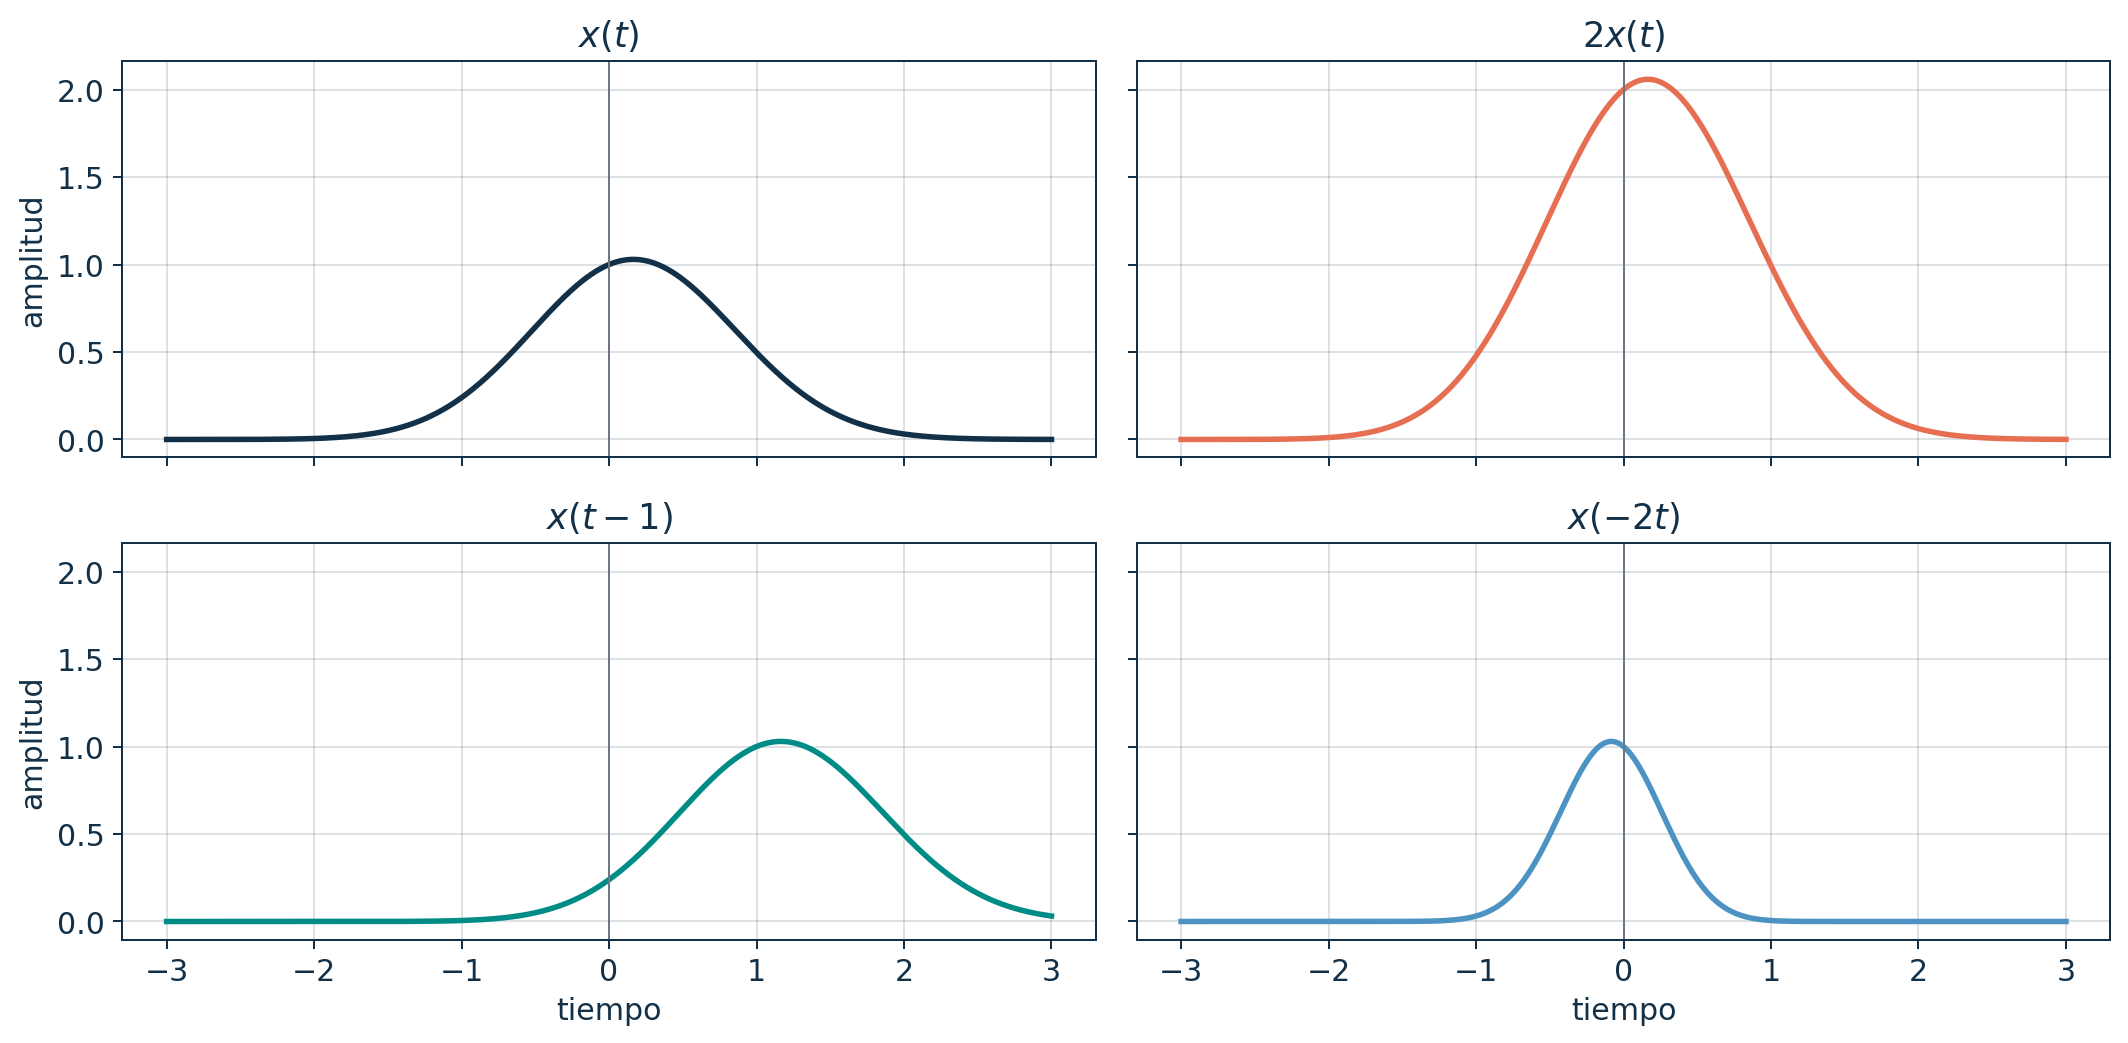
\includegraphics[width=0.82\linewidth,height=\textheight,keepaspectratio]{assets/10_transformations.png}

\begin{tcolorbox}[enhanced jigsaw, arc=.35mm, bottomrule=.15mm, bottomtitle=1mm, breakable, colback=white, colbacktitle=quarto-callout-tip-color!10!white, colframe=quarto-callout-tip-color-frame, coltitle=black, left=2mm, leftrule=.75mm, opacityback=0, opacitybacktitle=0.6, rightrule=.15mm, title={Método visual}, titlerule=0mm, toprule=.15mm, toptitle=1mm]

Identifique primero un punto notable: máximo, inicio o discontinuidad.
Después calcule su nueva ubicación y amplitud.

\end{tcolorbox}
\end{frame}

\begin{frame}[shrink]{Transformaciones combinadas}
\protect\phantomsection\label{transformaciones-combinadas}
Considere

\[y(t)=A\,x(at-b)+B.\]

Reescriba el argumento:

\[at-b=a\left(t-\frac{b}{a}\right).\]

Esto permite identificar:

\begin{enumerate}
\tightlist
\item
  desplazamiento efectivo \(b/a\);
\item
  escalamiento temporal por \(a\);
\item
  escalamiento vertical por \(A\);
\item
  desplazamiento vertical por \(B\).
\end{enumerate}

\begin{tcolorbox}[enhanced jigsaw, arc=.35mm, bottomrule=.15mm, bottomtitle=1mm, breakable, colback=white, colbacktitle=quarto-callout-caution-color!10!white, colframe=quarto-callout-caution-color-frame, coltitle=black, left=2mm, leftrule=.75mm, opacityback=0, opacitybacktitle=0.6, rightrule=.15mm, title={Orden de trabajo}, titlerule=0mm, toprule=.15mm, toptitle=1mm]

No lea \(b\) directamente como desplazamiento. Primero factorice el
coeficiente de \(t\).

\end{tcolorbox}
\end{frame}

\begin{frame}{Procedimiento con puntos notables}
\protect\phantomsection\label{procedimiento-con-puntos-notables}
Si un evento de \(x(t)\) ocurre en \(t=t_x\), en \(x(at-b)\) aparecerá
cuando

\[at-b=t_x,\]

por tanto,

\[t=\frac{t_x+b}{a}.\]

\begin{tcolorbox}[enhanced jigsaw, arc=.35mm, bottomrule=.15mm, bottomtitle=1mm, breakable, colback=white, colbacktitle=quarto-callout-important-color!10!white, colframe=quarto-callout-important-color-frame, coltitle=black, left=2mm, leftrule=.75mm, opacityback=0, opacitybacktitle=0.6, rightrule=.15mm, title={Ventaja}, titlerule=0mm, toprule=.15mm, toptitle=1mm]

Transformar coordenadas de puntos notables reduce errores de signo y
evita depender únicamente de una regla memorizada.

\end{tcolorbox}
\end{frame}

\begin{frame}{Señales pares e impares}
\protect\phantomsection\label{seuxf1ales-pares-e-impares}
Una señal es par cuando

\[x(-t)=x(t),\]

y es impar cuando

\[x(-t)=-x(t).\]

\begin{itemize}
\tightlist
\item
  Las señales pares presentan simetría respecto al eje vertical.
\item
  Las impares presentan simetría rotacional respecto al origen.
\end{itemize}

\begin{tcolorbox}[enhanced jigsaw, arc=.35mm, bottomrule=.15mm, bottomtitle=1mm, breakable, colback=white, colbacktitle=quarto-callout-note-color!10!white, colframe=quarto-callout-note-color-frame, coltitle=black, left=2mm, leftrule=.75mm, opacityback=0, opacitybacktitle=0.6, rightrule=.15mm, title={Ejemplos}, titlerule=0mm, toprule=.15mm, toptitle=1mm]

\(\cos(\omega t)\) es par y \(\sin(\omega t)\) es impar.

\end{tcolorbox}
\end{frame}

\begin{frame}[shrink]{Toda señal puede descomponerse}
\protect\phantomsection\label{toda-seuxf1al-puede-descomponerse}
Parte par:

\[x_e(t)=\frac{x(t)+x(-t)}{2}.\]

Parte impar:

\[x_o(t)=\frac{x(t)-x(-t)}{2}.\]

Reconstrucción:

\[x(t)=x_e(t)+x_o(t).\]

\begin{tcolorbox}[enhanced jigsaw, arc=.35mm, bottomrule=.15mm, bottomtitle=1mm, breakable, colback=white, colbacktitle=quarto-callout-important-color!10!white, colframe=quarto-callout-important-color-frame, coltitle=black, left=2mm, leftrule=.75mm, opacityback=0, opacitybacktitle=0.6, rightrule=.15mm, title={Propósito}, titlerule=0mm, toprule=.15mm, toptitle=1mm]

La descomposición separa simetrías y simplifica análisis posteriores,
especialmente en Fourier.

\end{tcolorbox}
\end{frame}

\begin{frame}{Descomposición par e impar}
\protect\phantomsection\label{descomposiciuxf3n-par-e-impar}
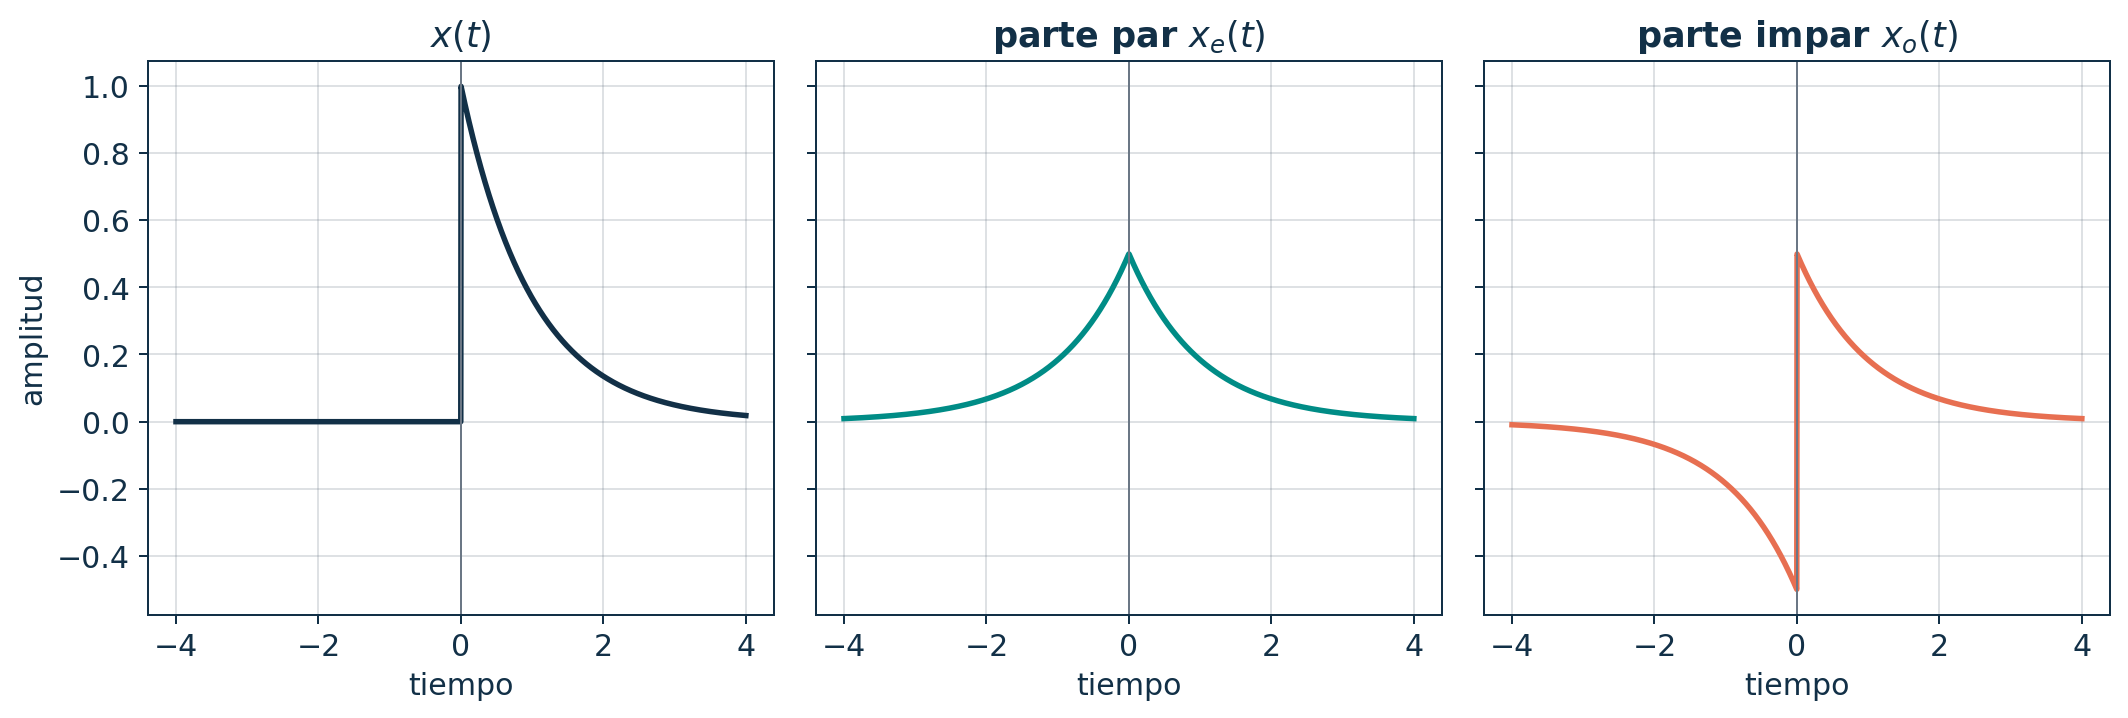
\includegraphics[width=0.94\linewidth,height=\textheight,keepaspectratio]{assets/11_even_odd.png}

\begin{tcolorbox}[enhanced jigsaw, arc=.35mm, bottomrule=.15mm, bottomtitle=1mm, breakable, colback=white, colbacktitle=quarto-callout-tip-color!10!white, colframe=quarto-callout-tip-color-frame, coltitle=black, left=2mm, leftrule=.75mm, opacityback=0, opacitybacktitle=0.6, rightrule=.15mm, title={Verificación}, titlerule=0mm, toprule=.15mm, toptitle=1mm]

Compruebe que \(x_e(-t)=x_e(t)\), \(x_o(-t)=-x_o(t)\) y que la suma
reconstruye \(x(t)\).

\end{tcolorbox}
\end{frame}

\begin{frame}[fragile]{Transformaciones mediante interpolación en
Python}
\protect\phantomsection\label{transformaciones-mediante-interpolaciuxf3n-en-python}
\begin{Shaded}
\begin{Highlighting}[]
\ImportTok{import}\NormalTok{ numpy }\ImportTok{as}\NormalTok{ np}

\CommentTok{\# x está muestreada sobre el eje t}
\KeywordTok{def}\NormalTok{ transform\_time(t, x, a}\OperatorTok{=}\FloatTok{1.0}\NormalTok{, b}\OperatorTok{=}\FloatTok{0.0}\NormalTok{):}
\NormalTok{    argument }\OperatorTok{=}\NormalTok{ a}\OperatorTok{*}\NormalTok{t }\OperatorTok{{-}}\NormalTok{ b}
    \ControlFlowTok{return}\NormalTok{ np.interp(argument, t, x,}
\NormalTok{                     left}\OperatorTok{=}\FloatTok{0.0}\NormalTok{, right}\OperatorTok{=}\FloatTok{0.0}\NormalTok{)}

\NormalTok{y\_shift }\OperatorTok{=}\NormalTok{ transform\_time(t, x, a}\OperatorTok{=}\DecValTok{1}\NormalTok{, b}\OperatorTok{=}\DecValTok{1}\NormalTok{)}
\NormalTok{y\_fold  }\OperatorTok{=}\NormalTok{ transform\_time(t, x, a}\OperatorTok{={-}}\DecValTok{1}\NormalTok{, b}\OperatorTok{=}\DecValTok{0}\NormalTok{)}
\end{Highlighting}
\end{Shaded}

\begin{tcolorbox}[enhanced jigsaw, arc=.35mm, bottomrule=.15mm, bottomtitle=1mm, breakable, colback=white, colbacktitle=quarto-callout-warning-color!10!white, colframe=quarto-callout-warning-color-frame, coltitle=black, left=2mm, leftrule=.75mm, opacityback=0, opacitybacktitle=0.6, rightrule=.15mm, title={Limitación numérica}, titlerule=0mm, toprule=.15mm, toptitle=1mm]

La interpolación aproxima valores entre muestras. Su error depende de la
frecuencia de muestreo y del método empleado.

\end{tcolorbox}
\end{frame}

\begin{frame}{Actividad: prediga antes de graficar}
\protect\phantomsection\label{actividad-prediga-antes-de-graficar}
Para una señal \(x(t)\) con máximo en \(t=1\) y amplitud máxima 2,
determine la posición y amplitud del máximo en:

\begin{enumerate}
\tightlist
\item
  \(y_1(t)=3x(t-2)\).
\item
  \(y_2(t)=x(2t-4)\).
\item
  \(y_3(t)=-x(-t)\).
\item
  \(y_4(t)=0.5x(0.5t+1)+2\).
\end{enumerate}

\begin{tcolorbox}[enhanced jigsaw, arc=.35mm, bottomrule=.15mm, bottomtitle=1mm, breakable, colback=white, colbacktitle=quarto-callout-tip-color!10!white, colframe=quarto-callout-tip-color-frame, coltitle=black, left=2mm, leftrule=.75mm, opacityback=0, opacitybacktitle=0.6, rightrule=.15mm, title={Secuencia recomendada}, titlerule=0mm, toprule=.15mm, toptitle=1mm]

Transforme primero la coordenada temporal del máximo; después aplique el
cambio de amplitud.

\end{tcolorbox}
\end{frame}

\begin{frame}{Cierre de la semana 3}
\protect\phantomsection\label{cierre-de-la-semana-3}
\begin{tcolorbox}[enhanced jigsaw, arc=.35mm, bottomrule=.15mm, bottomtitle=1mm, breakable, colback=white, colbacktitle=quarto-callout-important-color!10!white, colframe=quarto-callout-important-color-frame, coltitle=black, left=2mm, leftrule=.75mm, opacityback=0, opacitybacktitle=0.6, rightrule=.15mm, title={Síntesis}, titlerule=0mm, toprule=.15mm, toptitle=1mm]

Las transformaciones internas modifican el eje temporal; las externas
modifican amplitud. La factorización del argumento y el seguimiento de
puntos notables ofrecen un procedimiento verificable.

\end{tcolorbox}

\textbf{Preparación para la semana 4:} revise media, RMS, ventanas e
interpretación de eventos temporales.
\end{frame}

\section{Semana 4 · Sesión 1}\label{semana-4-sesiuxf3n-1}

\begin{frame}{El análisis temporal es una cadena de decisiones}
\protect\phantomsection\label{el-anuxe1lisis-temporal-es-una-cadena-de-decisiones}
Al finalizar esta sesión podrá:

\begin{itemize}
\tightlist
\item
  construir un flujo de análisis temporal;
\item
  detectar niveles basales, tendencias y eventos;
\item
  interpretar picos y cruces por cero con cautela;
\item
  estimar envolventes y magnitudes locales;
\item
  documentar decisiones de procesamiento.
\end{itemize}

\begin{tcolorbox}[enhanced jigsaw, arc=.35mm, bottomrule=.15mm, bottomtitle=1mm, breakable, colback=white, colbacktitle=quarto-callout-note-color!10!white, colframe=quarto-callout-note-color-frame, coltitle=black, left=2mm, leftrule=.75mm, opacityback=0, opacitybacktitle=0.6, rightrule=.15mm, title={Pregunta inicial}, titlerule=0mm, toprule=.15mm, toptitle=1mm]

¿Cuándo un máximo local representa un evento fisiológico y cuándo es
solo una fluctuación?

\end{tcolorbox}
\end{frame}

\begin{frame}{Flujo mínimo de análisis}
\protect\phantomsection\label{flujo-muxednimo-de-anuxe1lisis}
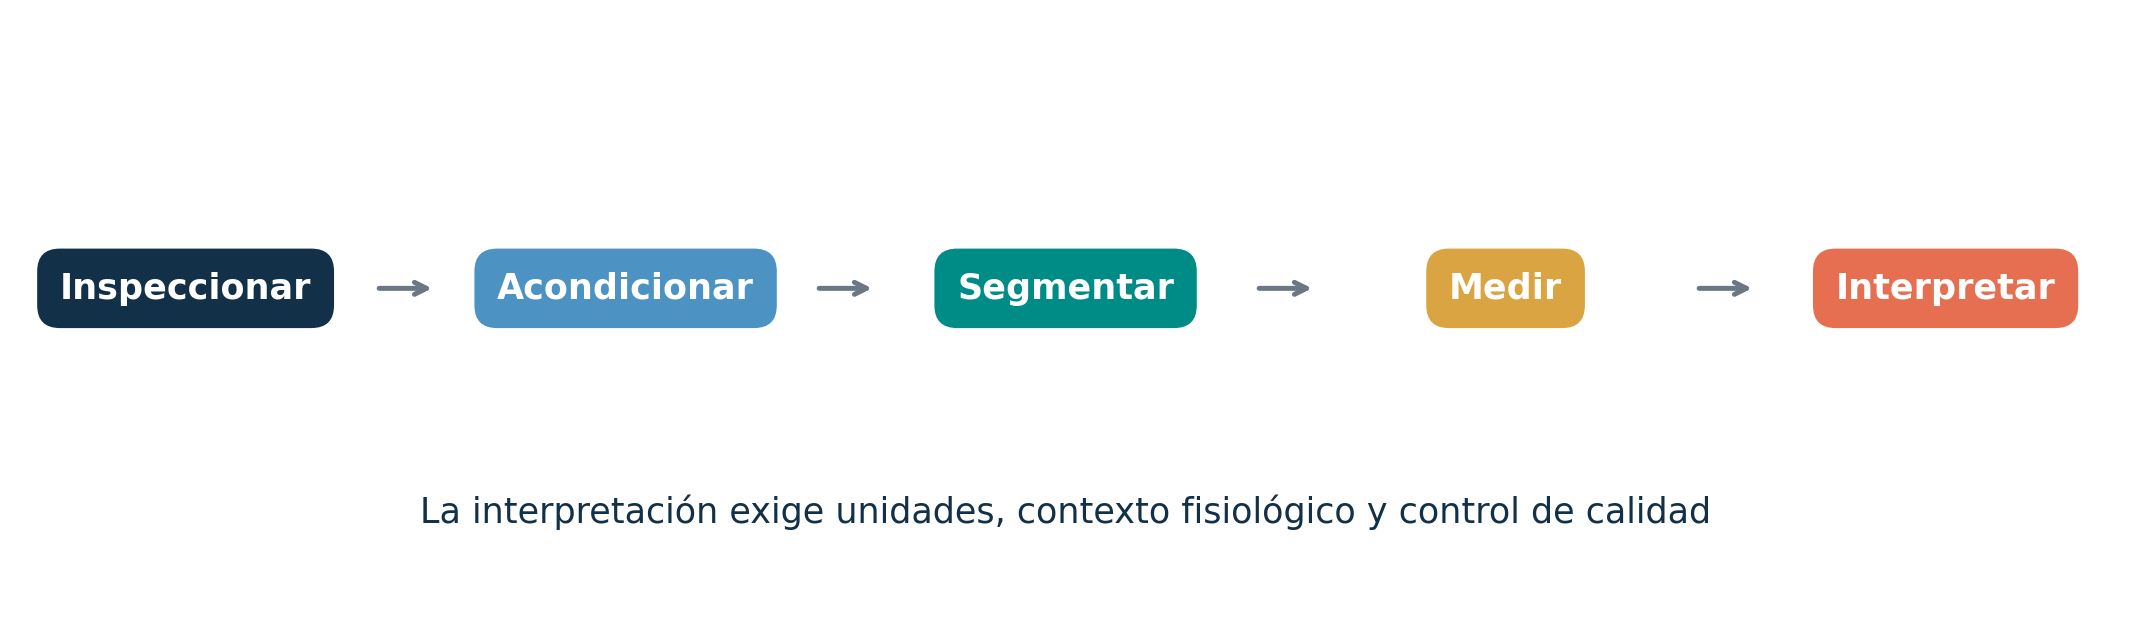
\includegraphics[width=0.95\linewidth,height=\textheight,keepaspectratio]{assets/12_time_workflow.png}

\begin{tcolorbox}[enhanced jigsaw, arc=.35mm, bottomrule=.15mm, bottomtitle=1mm, breakable, colback=white, colbacktitle=quarto-callout-important-color!10!white, colframe=quarto-callout-important-color-frame, coltitle=black, left=2mm, leftrule=.75mm, opacityback=0, opacitybacktitle=0.6, rightrule=.15mm, title={Orden lógico}, titlerule=0mm, toprule=.15mm, toptitle=1mm]

No extraiga características antes de verificar unidades, calidad,
valores ausentes, saturación y pertinencia de la ventana.

\end{tcolorbox}
\end{frame}

\begin{frame}{Inspección inicial: qué debe buscarse}
\protect\phantomsection\label{inspecciuxf3n-inicial-quuxe9-debe-buscarse}
\begin{enumerate}
\tightlist
\item
  Duración, frecuencia de muestreo y continuidad temporal.
\item
  Rango de amplitud y unidades.
\item
  Saturaciones o recortes.
\item
  Deriva lenta y cambios de nivel.
\item
  Eventos abruptos o valores aislados.
\item
  Segmentos faltantes.
\item
  Coherencia entre canales.
\end{enumerate}

\begin{tcolorbox}[enhanced jigsaw, arc=.35mm, bottomrule=.15mm, bottomtitle=1mm, breakable, colback=white, colbacktitle=quarto-callout-tip-color!10!white, colframe=quarto-callout-tip-color-frame, coltitle=black, left=2mm, leftrule=.75mm, opacityback=0, opacitybacktitle=0.6, rightrule=.15mm, title={Práctica recomendable}, titlerule=0mm, toprule=.15mm, toptitle=1mm]

Observe primero el registro completo y luego amplíe segmentos
representativos. Una sola escala puede ocultar problemas importantes.

\end{tcolorbox}
\end{frame}

\begin{frame}{Nivel basal y tendencia}
\protect\phantomsection\label{nivel-basal-y-tendencia}
Podemos representar una señal como

\[
x(t)=b(t)+r(t),
\]

donde \(b(t)\) es una componente lenta y \(r(t)\) contiene variaciones
más rápidas.

\begin{itemize}
\tightlist
\item
  El nivel basal puede tener significado fisiológico.
\item
  También puede reflejar desplazamiento instrumental.
\item
  La tendencia puede ser parte del fenómeno o una contaminación.
\end{itemize}

\begin{tcolorbox}[enhanced jigsaw, arc=.35mm, bottomrule=.15mm, bottomtitle=1mm, breakable, colback=white, colbacktitle=quarto-callout-warning-color!10!white, colframe=quarto-callout-warning-color-frame, coltitle=black, left=2mm, leftrule=.75mm, opacityback=0, opacitybacktitle=0.6, rightrule=.15mm, title={No elimine sin justificar}, titlerule=0mm, toprule=.15mm, toptitle=1mm]

Restar la media o eliminar una tendencia modifica la señal. La decisión
debe corresponder a la pregunta de análisis.

\end{tcolorbox}
\end{frame}

\begin{frame}[shrink]{Detectar picos es aplicar criterios}
\protect\phantomsection\label{detectar-picos-es-aplicar-criterios}
Un máximo local \(x[n]\) satisface, en su forma más simple,

\[x[n]>x[n-1],\qquad x[n]\geq x[n+1].\]

En aplicaciones reales también se requieren criterios como:

\begin{itemize}
\tightlist
\item
  altura mínima;
\item
  prominencia;
\item
  distancia entre picos;
\item
  anchura;
\item
  contexto morfológico.
\end{itemize}

\begin{tcolorbox}[enhanced jigsaw, arc=.35mm, bottomrule=.15mm, bottomtitle=1mm, breakable, colback=white, colbacktitle=quarto-callout-important-color!10!white, colframe=quarto-callout-important-color-frame, coltitle=black, left=2mm, leftrule=.75mm, opacityback=0, opacitybacktitle=0.6, rightrule=.15mm, title={Concepto}, titlerule=0mm, toprule=.15mm, toptitle=1mm]

El detector produce candidatos matemáticos. La validación fisiológica
determina cuáles corresponden al evento de interés.

\end{tcolorbox}
\end{frame}

\begin{frame}[shrink]{Un detector puede acertar matemáticamente y fallar
fisiológicamente}
\protect\phantomsection\label{un-detector-puede-acertar-matemuxe1ticamente-y-fallar-fisioluxf3gicamente}
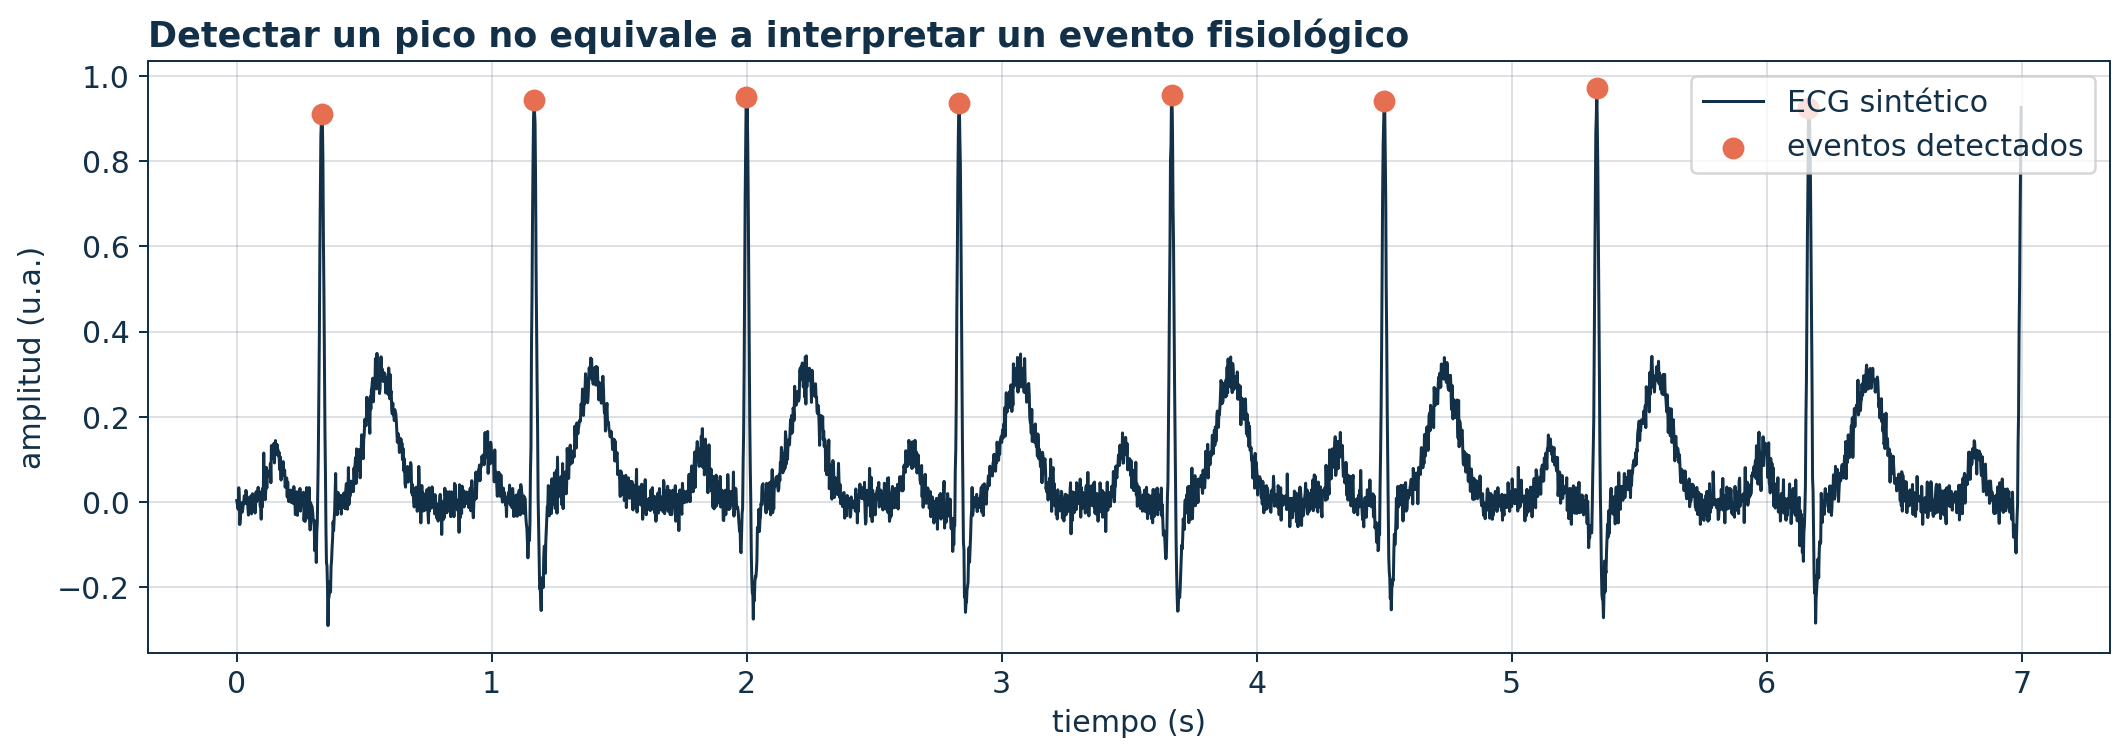
\includegraphics[width=0.88\linewidth,height=\textheight,keepaspectratio]{assets/13_peak_detection.png}

\begin{tcolorbox}[enhanced jigsaw, arc=.35mm, bottomrule=.15mm, bottomtitle=1mm, breakable, colback=white, colbacktitle=quarto-callout-caution-color!10!white, colframe=quarto-callout-caution-color-frame, coltitle=black, left=2mm, leftrule=.75mm, opacityback=0, opacitybacktitle=0.6, rightrule=.15mm, title={Límite de interpretación}, titlerule=0mm, toprule=.15mm, toptitle=1mm]

Una marca sobre un pico no demuestra que sea una onda específica, un
latido válido o un hallazgo clínico.

\end{tcolorbox}
\end{frame}

\begin{frame}[fragile]{Detección de picos en Python}
\protect\phantomsection\label{detecciuxf3n-de-picos-en-python}
\begin{Shaded}
\begin{Highlighting}[]
\ImportTok{from}\NormalTok{ scipy.signal }\ImportTok{import}\NormalTok{ find\_peaks}

\NormalTok{min\_distance }\OperatorTok{=} \BuiltInTok{int}\NormalTok{(}\FloatTok{0.60} \OperatorTok{*}\NormalTok{ fs)}
\NormalTok{peaks, properties }\OperatorTok{=}\NormalTok{ find\_peaks(}
\NormalTok{    x,}
\NormalTok{    distance}\OperatorTok{=}\NormalTok{min\_distance,}
\NormalTok{    prominence}\OperatorTok{=}\FloatTok{0.55}\NormalTok{,}
\NormalTok{)}

\NormalTok{event\_times }\OperatorTok{=}\NormalTok{ peaks }\OperatorTok{/}\NormalTok{ fs}
\end{Highlighting}
\end{Shaded}

\begin{tcolorbox}[enhanced jigsaw, arc=.35mm, bottomrule=.15mm, bottomtitle=1mm, breakable, colback=white, colbacktitle=quarto-callout-tip-color!10!white, colframe=quarto-callout-tip-color-frame, coltitle=black, left=2mm, leftrule=.75mm, opacityback=0, opacitybacktitle=0.6, rightrule=.15mm, title={Parámetros con unidades}, titlerule=0mm, toprule=.15mm, toptitle=1mm]

Convierta duraciones fisiológicamente justificadas a muestras. No copie
valores de \texttt{distance} entre señales con diferente \(f_s\).

\end{tcolorbox}
\end{frame}

\begin{frame}{Cruces por cero}
\protect\phantomsection\label{cruces-por-cero}
Un cruce ocurre cuando cambia el signo:

\[x[n]x[n-1]<0.\]

Conteo simple:

\[
Z=\sum_{n=1}^{N-1}\mathbf{1}\{x[n]x[n-1]<0\}.
\]

\begin{tcolorbox}[enhanced jigsaw, arc=.35mm, bottomrule=.15mm, bottomtitle=1mm, breakable, colback=white, colbacktitle=quarto-callout-warning-color!10!white, colframe=quarto-callout-warning-color-frame, coltitle=black, left=2mm, leftrule=.75mm, opacityback=0, opacitybacktitle=0.6, rightrule=.15mm, title={Sensibilidad al ruido}, titlerule=0mm, toprule=.15mm, toptitle=1mm]

Pequeñas fluctuaciones alrededor de cero pueden producir muchos cruces.
Es habitual usar umbrales, histéresis o preprocesamiento.

\end{tcolorbox}
\end{frame}

\begin{frame}{La rectificación cambia la representación}
\protect\phantomsection\label{la-rectificaciuxf3n-cambia-la-representaciuxf3n}
Rectificación de onda completa:

\[x_r[n]=|x[n]|.\]

La rectificación:

\begin{itemize}
\tightlist
\item
  hace no negativas las amplitudes;
\item
  permite resumir magnitud local;
\item
  introduce una componente de baja frecuencia;
\item
  altera el contenido espectral original.
\end{itemize}

\begin{tcolorbox}[enhanced jigsaw, arc=.35mm, bottomrule=.15mm, bottomtitle=1mm, breakable, colback=white, colbacktitle=quarto-callout-caution-color!10!white, colframe=quarto-callout-caution-color-frame, coltitle=black, left=2mm, leftrule=.75mm, opacityback=0, opacitybacktitle=0.6, rightrule=.15mm, title={Interpretación}, titlerule=0mm, toprule=.15mm, toptitle=1mm]

Una señal rectificada ya no conserva polaridad. No debe tratarse como si
fuera el registro original.

\end{tcolorbox}
\end{frame}

\begin{frame}[shrink]{Envolvente de una señal oscilatoria}
\protect\phantomsection\label{envolvente-de-una-seuxf1al-oscilatoria}
Una aproximación frecuente consiste en rectificar y suavizar:

\[e[n]=\mathcal{L}\{|x[n]|\},\]

donde \(\mathcal{L}\) representa un filtro pasa bajas.

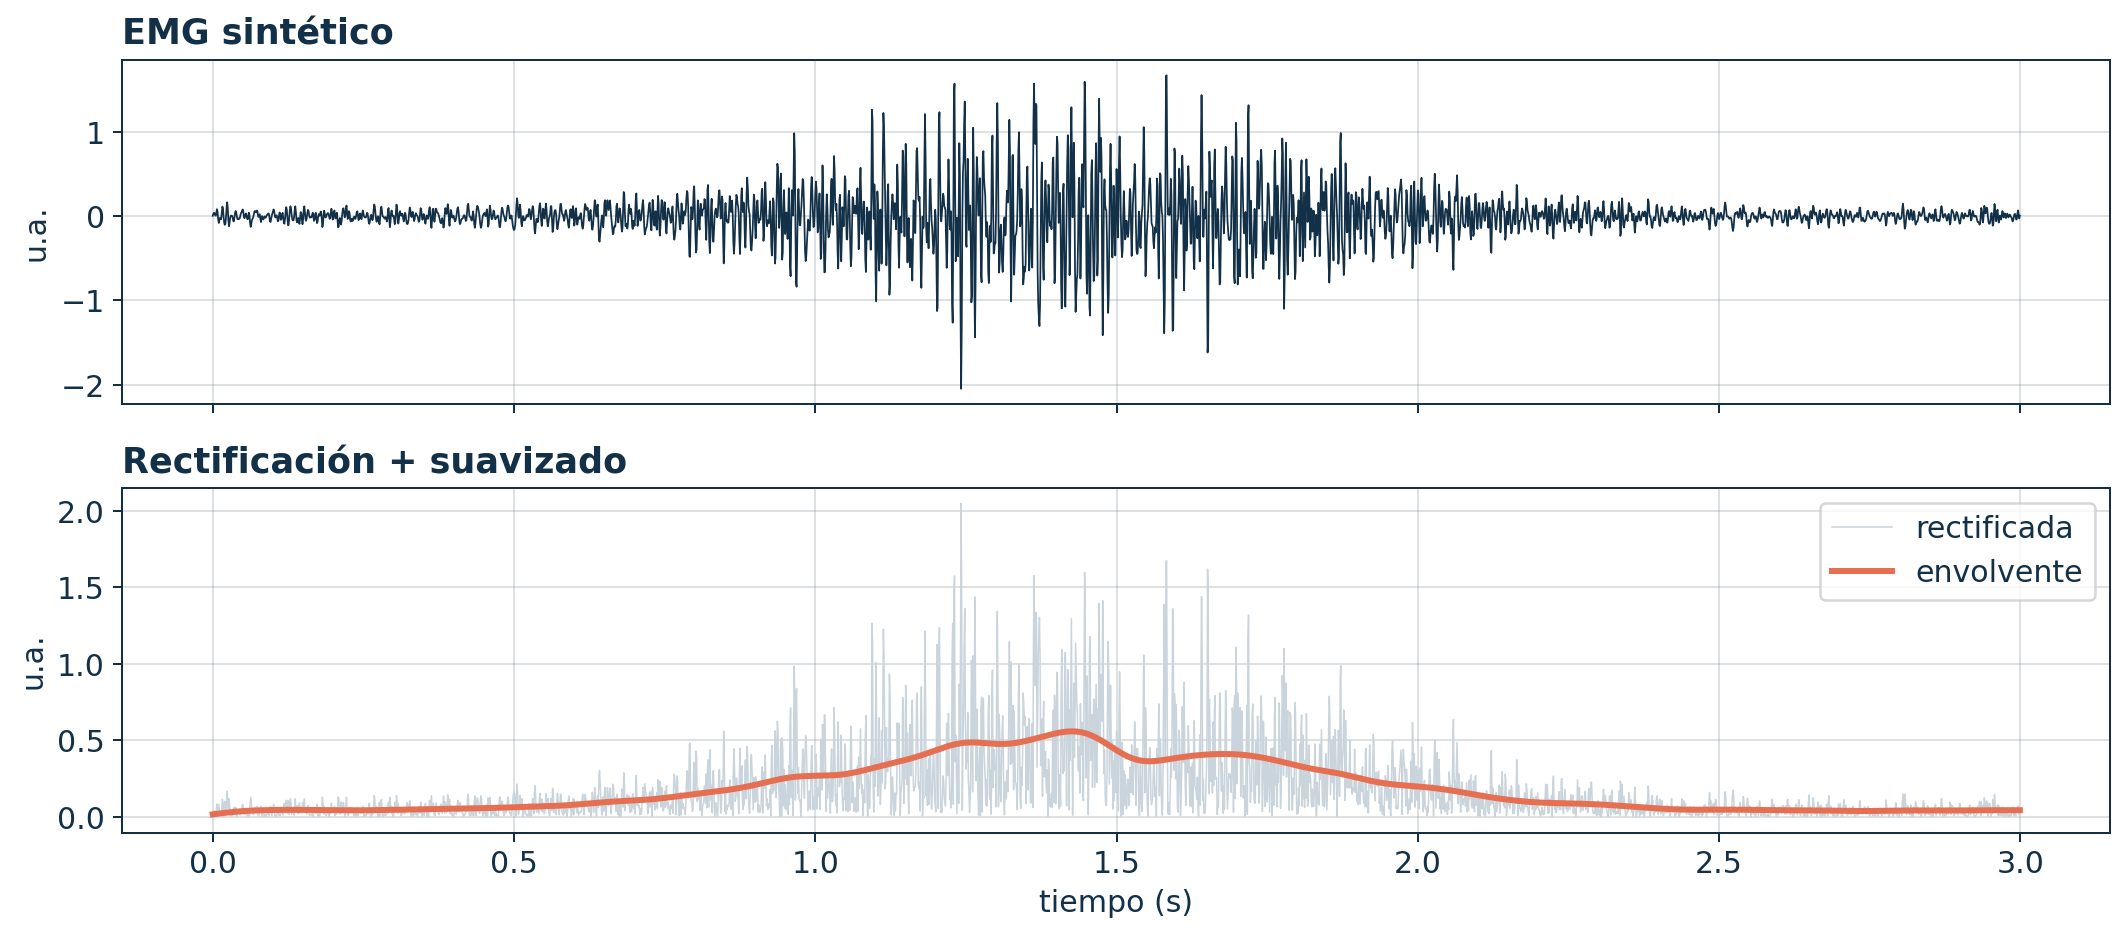
\includegraphics[width=0.78\linewidth,height=\textheight,keepaspectratio]{assets/14_envelope.png}

\begin{tcolorbox}[enhanced jigsaw, arc=.35mm, bottomrule=.15mm, bottomtitle=1mm, breakable, colback=white, colbacktitle=quarto-callout-note-color!10!white, colframe=quarto-callout-note-color-frame, coltitle=black, left=2mm, leftrule=.75mm, opacityback=0, opacitybacktitle=0.6, rightrule=.15mm, title={Qué representa}, titlerule=0mm, toprule=.15mm, toptitle=1mm]

La envolvente describe cambios lentos de magnitud; no es equivalente a
la forma de onda EMG ni a la fuerza muscular.

\end{tcolorbox}
\end{frame}

\begin{frame}{RMS móvil y envolvente no son idénticos}
\protect\phantomsection\label{rms-muxf3vil-y-envolvente-no-son-iduxe9nticos}
{\def\LTcaptype{none} % do not increment counter
\begin{longtable}[]{@{}
  >{\raggedright\arraybackslash}p{(\linewidth - 6\tabcolsep) * \real{0.2500}}
  >{\raggedright\arraybackslash}p{(\linewidth - 6\tabcolsep) * \real{0.2500}}
  >{\raggedright\arraybackslash}p{(\linewidth - 6\tabcolsep) * \real{0.2500}}
  >{\raggedright\arraybackslash}p{(\linewidth - 6\tabcolsep) * \real{0.2500}}@{}}
\toprule\noalign{}
\begin{minipage}[b]{\linewidth}\raggedright
Método
\end{minipage} & \begin{minipage}[b]{\linewidth}\raggedright
Operación
\end{minipage} & \begin{minipage}[b]{\linewidth}\raggedright
Ventaja
\end{minipage} & \begin{minipage}[b]{\linewidth}\raggedright
Precaución
\end{minipage} \\
\midrule\noalign{}
\endhead
RMS móvil & cuadrado → promedio → raíz & conserva interpretación
cuadrática & depende de ventana \\
Rectificación + pasa bajas & valor absoluto → suavizado & intuitivo y
continuo & depende del filtro \\
Envolvente de Hilbert & magnitud de señal analítica & útil en señales
estrechas en banda & requiere supuestos espectrales \\
\bottomrule\noalign{}
\end{longtable}
}

\begin{tcolorbox}[enhanced jigsaw, arc=.35mm, bottomrule=.15mm, bottomtitle=1mm, breakable, colback=white, colbacktitle=quarto-callout-important-color!10!white, colframe=quarto-callout-important-color-frame, coltitle=black, left=2mm, leftrule=.75mm, opacityback=0, opacitybacktitle=0.6, rightrule=.15mm, title={Selección}, titlerule=0mm, toprule=.15mm, toptitle=1mm]

Elija el método según la estructura de la señal y la pregunta, no por
costumbre.

\end{tcolorbox}
\end{frame}

\begin{frame}{Actividad: diseñe criterios de evento}
\protect\phantomsection\label{actividad-diseuxf1e-criterios-de-evento}
Se desea detectar el inicio de una contracción en EMG superficial.

Proponga:

\begin{enumerate}
\tightlist
\item
  representación empleada: cruda, rectificada, RMS o envolvente;
\item
  duración de ventana;
\item
  umbral y referencia basal;
\item
  duración mínima del evento;
\item
  criterio para rechazar artefactos;
\item
  procedimiento de validación.
\end{enumerate}

\begin{tcolorbox}[enhanced jigsaw, arc=.35mm, bottomrule=.15mm, bottomtitle=1mm, breakable, colback=white, colbacktitle=quarto-callout-tip-color!10!white, colframe=quarto-callout-tip-color-frame, coltitle=black, left=2mm, leftrule=.75mm, opacityback=0, opacitybacktitle=0.6, rightrule=.15mm, title={Criterio de evaluación}, titlerule=0mm, toprule=.15mm, toptitle=1mm]

La respuesta debe justificar cada parámetro y reconocer que el inicio
estimado depende del método.

\end{tcolorbox}
\end{frame}

\begin{frame}{Cierre de la sesión 7}
\protect\phantomsection\label{cierre-de-la-sesiuxf3n-7}
\begin{tcolorbox}[enhanced jigsaw, arc=.35mm, bottomrule=.15mm, bottomtitle=1mm, breakable, colback=white, colbacktitle=quarto-callout-important-color!10!white, colframe=quarto-callout-important-color-frame, coltitle=black, left=2mm, leftrule=.75mm, opacityback=0, opacitybacktitle=0.6, rightrule=.15mm, title={Síntesis}, titlerule=0mm, toprule=.15mm, toptitle=1mm]

Picos, cruces, RMS y envolventes son construcciones matemáticas. Su
validez depende del preprocesamiento, los parámetros y la
correspondencia con el evento fisiológico.

\end{tcolorbox}

\textbf{Conexión:} una característica local requiere definir con
precisión qué segmento de señal representa cada condición.
\end{frame}

\section{Semana 4 · Sesión 2}\label{semana-4-sesiuxf3n-2}

\begin{frame}{Segmentar es decidir qué observaciones se comparan}
\protect\phantomsection\label{segmentar-es-decidir-quuxe9-observaciones-se-comparan}
Al finalizar esta sesión podrá:

\begin{itemize}
\tightlist
\item
  elegir entre segmentación por eventos y por ventanas;
\item
  comprender longitud y solapamiento;
\item
  normalizar sin perder trazabilidad;
\item
  construir tablas de características;
\item
  evaluar comparabilidad y posibles fugas de información.
\end{itemize}

\begin{tcolorbox}[enhanced jigsaw, arc=.35mm, bottomrule=.15mm, bottomtitle=1mm, breakable, colback=white, colbacktitle=quarto-callout-note-color!10!white, colframe=quarto-callout-note-color-frame, coltitle=black, left=2mm, leftrule=.75mm, opacityback=0, opacitybacktitle=0.6, rightrule=.15mm, title={Pregunta inicial}, titlerule=0mm, toprule=.15mm, toptitle=1mm]

¿Dos ventanas extraídas del mismo sujeto representan dos observaciones
independientes?

\end{tcolorbox}
\end{frame}

\begin{frame}[shrink]{Estrategias de segmentación}
\protect\phantomsection\label{estrategias-de-segmentaciuxf3n}
{\def\LTcaptype{none} % do not increment counter
\begin{longtable}[]{@{}
  >{\raggedright\arraybackslash}p{(\linewidth - 6\tabcolsep) * \real{0.2500}}
  >{\raggedright\arraybackslash}p{(\linewidth - 6\tabcolsep) * \real{0.2500}}
  >{\raggedright\arraybackslash}p{(\linewidth - 6\tabcolsep) * \real{0.2500}}
  >{\raggedright\arraybackslash}p{(\linewidth - 6\tabcolsep) * \real{0.2500}}@{}}
\toprule\noalign{}
\begin{minipage}[b]{\linewidth}\raggedright
Estrategia
\end{minipage} & \begin{minipage}[b]{\linewidth}\raggedright
Referencia
\end{minipage} & \begin{minipage}[b]{\linewidth}\raggedright
Ventaja
\end{minipage} & \begin{minipage}[b]{\linewidth}\raggedright
Riesgo
\end{minipage} \\
\midrule\noalign{}
\endhead
Por evento & marcador fisiológico o experimental & alineación
interpretable & error de detección \\
Ventanas fijas & duración constante & implementación sencilla & mezcla
de estados \\
Ventanas deslizantes & longitud y solapamiento & seguimiento temporal &
observaciones correlacionadas \\
Ciclos & periodo estimado & comparación morfológica & variabilidad y
ciclos inválidos \\
\bottomrule\noalign{}
\end{longtable}
}

\begin{tcolorbox}[enhanced jigsaw, arc=.35mm, bottomrule=.15mm, bottomtitle=1mm, breakable, colback=white, colbacktitle=quarto-callout-important-color!10!white, colframe=quarto-callout-important-color-frame, coltitle=black, left=2mm, leftrule=.75mm, opacityback=0, opacitybacktitle=0.6, rightrule=.15mm, title={Concepto}, titlerule=0mm, toprule=.15mm, toptitle=1mm]

La segmentación define la unidad de análisis. Por eso afecta
directamente la validez estadística y biomédica.

\end{tcolorbox}
\end{frame}

\begin{frame}[shrink]{Longitud y solapamiento}
\protect\phantomsection\label{longitud-y-solapamiento}
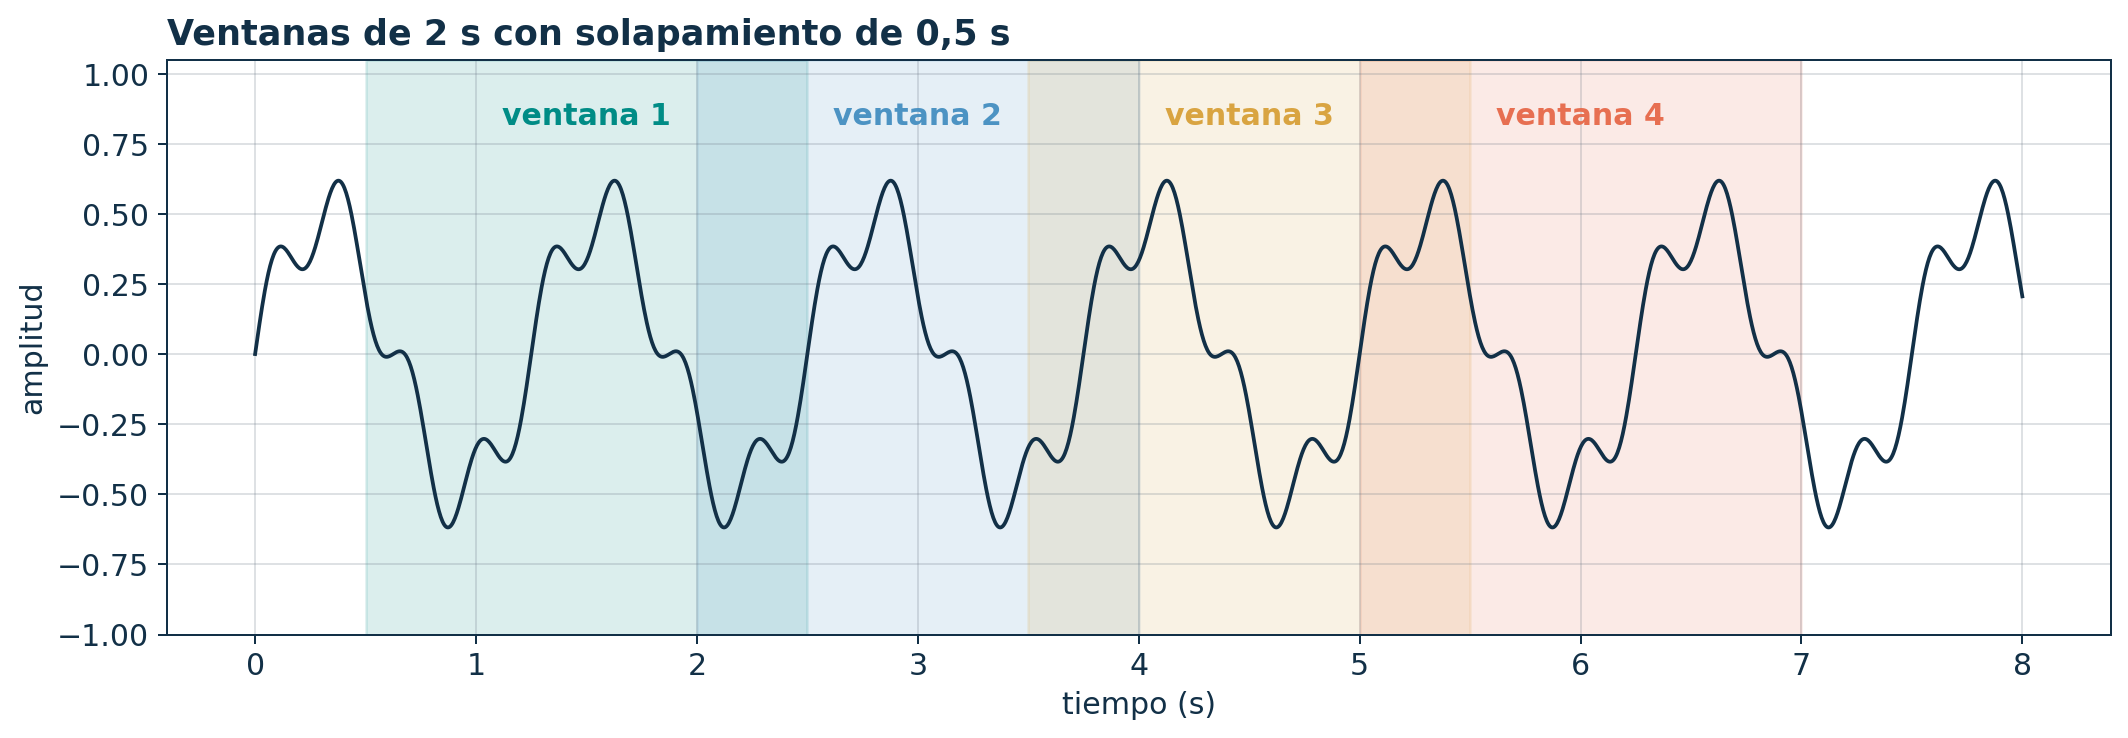
\includegraphics[width=0.82\linewidth,height=\textheight,keepaspectratio]{assets/15_segmentation.png}

Si una ventana tiene \(L\) muestras y el avance es \(R\), el
solapamiento es

\[
O=1-\frac{R}{L}.
\]

\begin{tcolorbox}[enhanced jigsaw, arc=.35mm, bottomrule=.15mm, bottomtitle=1mm, breakable, colback=white, colbacktitle=quarto-callout-warning-color!10!white, colframe=quarto-callout-warning-color-frame, coltitle=black, left=2mm, leftrule=.75mm, opacityback=0, opacitybacktitle=0.6, rightrule=.15mm, title={Dependencia}, titlerule=0mm, toprule=.15mm, toptitle=1mm]

Un solapamiento elevado produce ventanas muy similares. No deben
tratarse automáticamente como observaciones independientes.

\end{tcolorbox}
\end{frame}

\begin{frame}{La ventana debe contener el fenómeno relevante}
\protect\phantomsection\label{la-ventana-debe-contener-el-fenuxf3meno-relevante}
Una ventana demasiado corta puede:

\begin{itemize}
\tightlist
\item
  dividir un evento;
\item
  producir métricas inestables;
\item
  perder componentes lentas.
\end{itemize}

Una ventana demasiado larga puede:

\begin{itemize}
\tightlist
\item
  mezclar estados fisiológicos;
\item
  diluir eventos transitorios;
\item
  ocultar cambios temporales.
\end{itemize}

\begin{tcolorbox}[enhanced jigsaw, arc=.35mm, bottomrule=.15mm, bottomtitle=1mm, breakable, colback=white, colbacktitle=quarto-callout-note-color!10!white, colframe=quarto-callout-note-color-frame, coltitle=black, left=2mm, leftrule=.75mm, opacityback=0, opacitybacktitle=0.6, rightrule=.15mm, title={Criterio de selección}, titlerule=0mm, toprule=.15mm, toptitle=1mm]

La longitud debe justificarse usando la escala temporal del fenómeno y
la resolución requerida.

\end{tcolorbox}
\end{frame}

\begin{frame}[shrink]{Normalizar no corrige una adquisición deficiente}
\protect\phantomsection\label{normalizar-no-corrige-una-adquisiciuxf3n-deficiente}
Tres transformaciones comunes:

\[
x_c[n]=x[n]-\bar{x},
\]

\[
z[n]=\frac{x[n]-\bar{x}}{\sigma_x},
\]

\[
x_{01}[n]=\frac{x[n]-x_{\min}}{x_{\max}-x_{\min}}.
\]

\begin{tcolorbox}[enhanced jigsaw, arc=.35mm, bottomrule=.15mm, bottomtitle=1mm, breakable, colback=white, colbacktitle=quarto-callout-warning-color!10!white, colframe=quarto-callout-warning-color-frame, coltitle=black, left=2mm, leftrule=.75mm, opacityback=0, opacitybacktitle=0.6, rightrule=.15mm, title={Pérdida de interpretación}, titlerule=0mm, toprule=.15mm, toptitle=1mm]

Después de estandarizar o escalar, la amplitud deja de conservar las
unidades físicas originales.

\end{tcolorbox}
\end{frame}

\begin{frame}[shrink]{Tres escalas, una misma forma relativa}
\protect\phantomsection\label{tres-escalas-una-misma-forma-relativa}
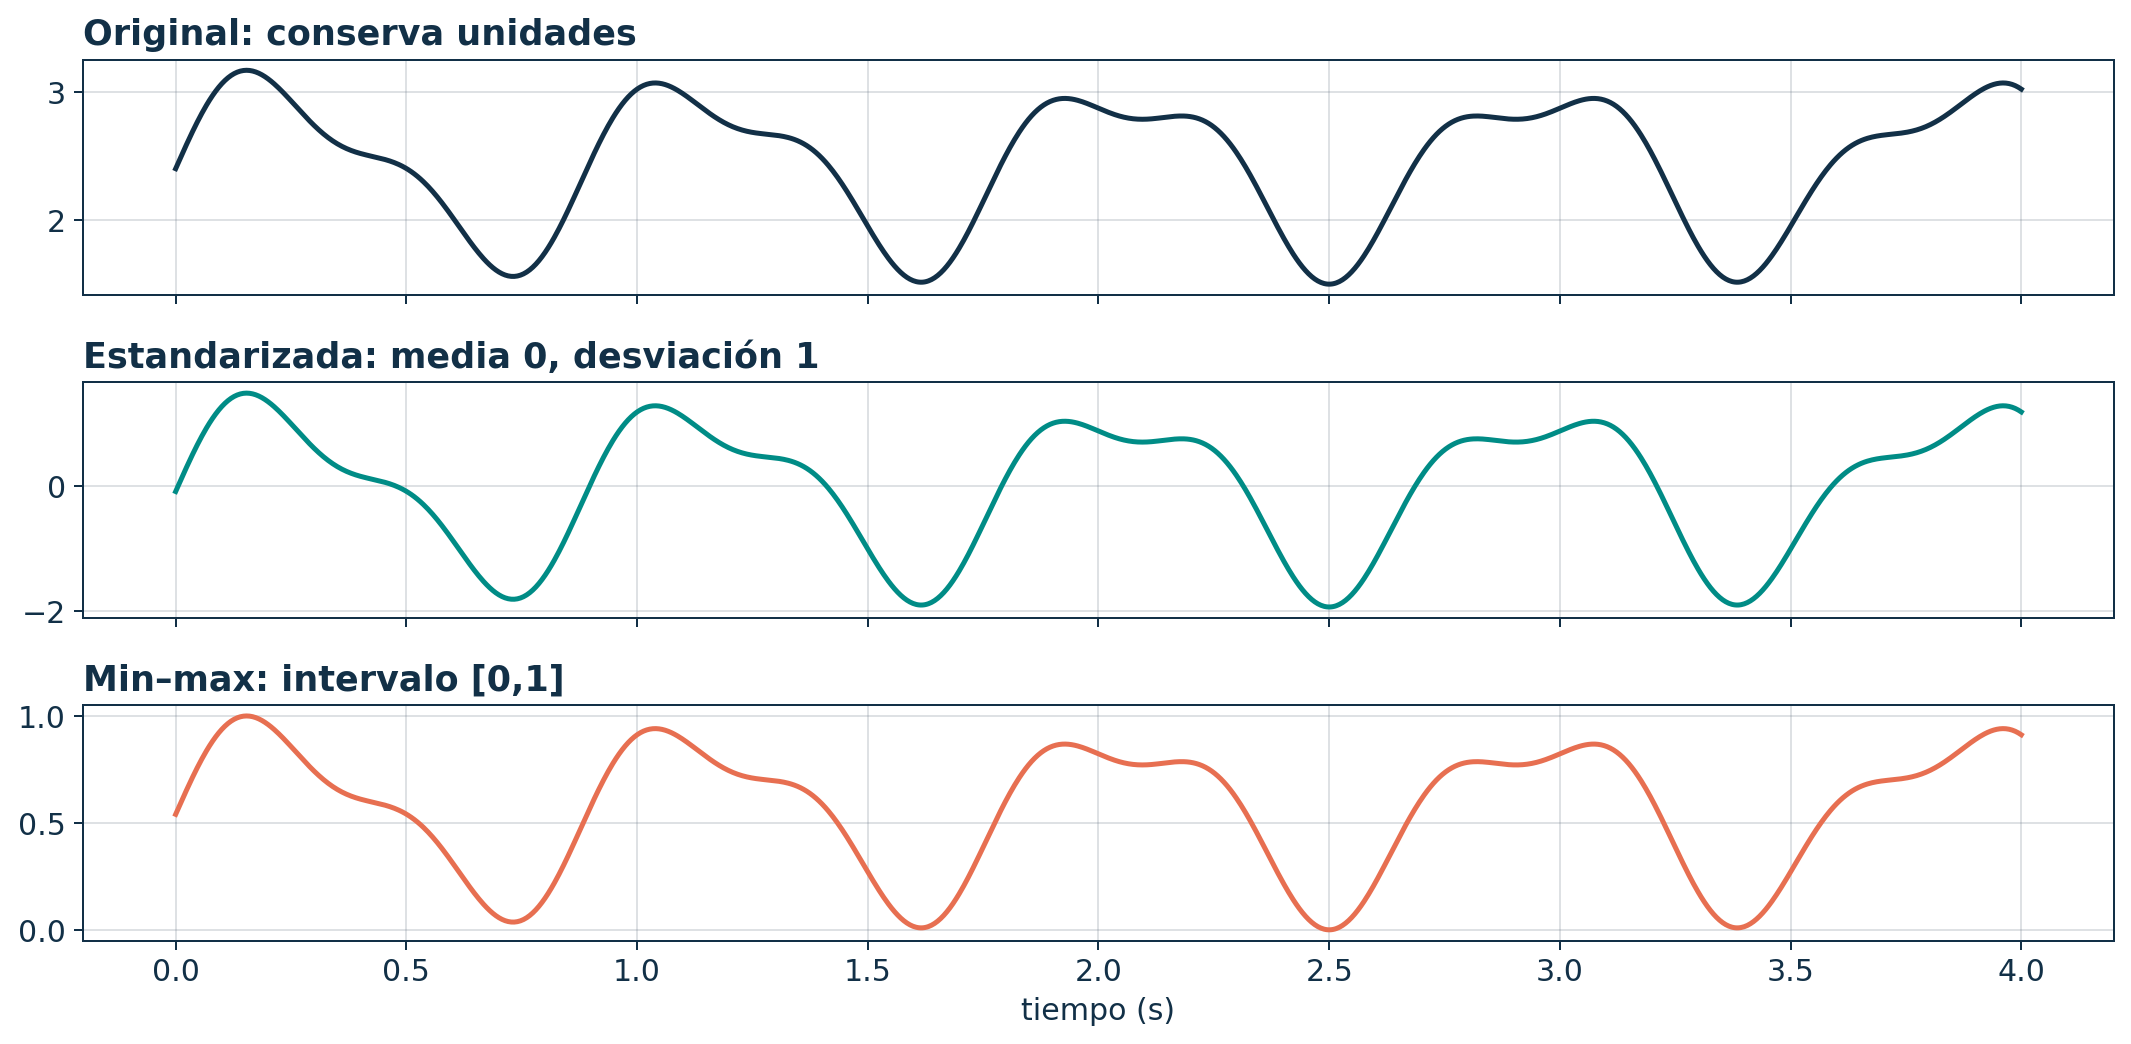
\includegraphics[width=0.8\linewidth,height=\textheight,keepaspectratio]{assets/16_normalization.png}

\begin{tcolorbox}[enhanced jigsaw, arc=.35mm, bottomrule=.15mm, bottomtitle=1mm, breakable, colback=white, colbacktitle=quarto-callout-important-color!10!white, colframe=quarto-callout-important-color-frame, coltitle=black, left=2mm, leftrule=.75mm, opacityback=0, opacitybacktitle=0.6, rightrule=.15mm, title={Distinción}, titlerule=0mm, toprule=.15mm, toptitle=1mm]

La normalización cambia la escala; no elimina ruido, artefactos, sesgo
ni falta de comparabilidad experimental.

\end{tcolorbox}
\end{frame}

\begin{frame}{Normalización global o local}
\protect\phantomsection\label{normalizaciuxf3n-global-o-local}
\begin{columns}[T]
\begin{column}{0.48\linewidth}
\begin{block}{Global}
\protect\phantomsection\label{global}
Usa parámetros calculados sobre un conjunto amplio.

\begin{itemize}
\tightlist
\item
  Facilita comparación entre ventanas.
\item
  Puede verse afectada por heterogeneidad.
\item
  En aprendizaje automático debe calcularse solo con entrenamiento.
\end{itemize}
\end{block}
\end{column}

\begin{column}{0.48\linewidth}
\begin{block}{Local}
\protect\phantomsection\label{local}
Usa parámetros de cada ventana o sujeto.

\begin{itemize}
\tightlist
\item
  Reduce diferencias de escala.
\item
  Puede borrar cambios absolutos relevantes.
\item
  Hace que cada segmento tenga una referencia distinta.
\end{itemize}
\end{block}
\end{column}
\end{columns}

\begin{tcolorbox}[enhanced jigsaw, arc=.35mm, bottomrule=.15mm, bottomtitle=1mm, breakable, colback=white, colbacktitle=quarto-callout-caution-color!10!white, colframe=quarto-callout-caution-color-frame, coltitle=black, left=2mm, leftrule=.75mm, opacityback=0, opacitybacktitle=0.6, rightrule=.15mm, title={Fuga de información}, titlerule=0mm, toprule=.15mm, toptitle=1mm]

Calcular parámetros de normalización usando datos de prueba introduce
información futura en el entrenamiento.

\end{tcolorbox}
\end{frame}

\begin{frame}[shrink]{De la señal a una matriz de características}
\protect\phantomsection\label{de-la-seuxf1al-a-una-matriz-de-caracteruxedsticas}
Para \(K\) segmentos y \(P\) características:

\[
\mathbf{F}=
\begin{bmatrix}
f_{11}&\cdots&f_{1P}\\
\vdots&\ddots&\vdots\\
f_{K1}&\cdots&f_{KP}
\end{bmatrix}.
\]

Cada fila debe conservar identificadores como:

\begin{itemize}
\tightlist
\item
  sujeto;
\item
  sesión y condición;
\item
  canal;
\item
  instante inicial y final;
\item
  versión de procesamiento.
\end{itemize}

\begin{tcolorbox}[enhanced jigsaw, arc=.35mm, bottomrule=.15mm, bottomtitle=1mm, breakable, colback=white, colbacktitle=quarto-callout-important-color!10!white, colframe=quarto-callout-important-color-frame, coltitle=black, left=2mm, leftrule=.75mm, opacityback=0, opacitybacktitle=0.6, rightrule=.15mm, title={Trazabilidad}, titlerule=0mm, toprule=.15mm, toptitle=1mm]

Una característica sin vínculo con su segmento de origen no puede
auditarse ni reinterpretarse.

\end{tcolorbox}
\end{frame}

\begin{frame}{Ejemplo de tabla analítica}
\protect\phantomsection\label{ejemplo-de-tabla-analuxedtica}
{\def\LTcaptype{none} % do not increment counter
\begin{longtable}[]{@{}lrlrrrl@{}}
\toprule\noalign{}
Sujeto & Sesión & Canal & Inicio (s) & Fin (s) & RMS (mV) & Calidad \\
\midrule\noalign{}
\endhead
P01 & 1 & EMG-TA & 12.0 & 14.0 & valor calculado & válida \\
P01 & 1 & EMG-TA & 13.5 & 15.5 & valor calculado & revisar \\
P02 & 1 & EMG-TA & 12.0 & 14.0 & valor calculado & válida \\
\bottomrule\noalign{}
\end{longtable}
}

\begin{tcolorbox}[enhanced jigsaw, arc=.35mm, bottomrule=.15mm, bottomtitle=1mm, breakable, colback=white, colbacktitle=quarto-callout-note-color!10!white, colframe=quarto-callout-note-color-frame, coltitle=black, left=2mm, leftrule=.75mm, opacityback=0, opacitybacktitle=0.6, rightrule=.15mm, title={Diseño correcto}, titlerule=0mm, toprule=.15mm, toptitle=1mm]

La tabla separa metadatos, características y control de calidad. No
reemplaza los segmentos originales.

\end{tcolorbox}
\end{frame}

\begin{frame}[shrink]{Características según el tipo de señal}
\protect\phantomsection\label{caracteruxedsticas-seguxfan-el-tipo-de-seuxf1al}
{\def\LTcaptype{none} % do not increment counter
\begin{longtable}[]{@{}
  >{\raggedright\arraybackslash}p{(\linewidth - 4\tabcolsep) * \real{0.3333}}
  >{\raggedright\arraybackslash}p{(\linewidth - 4\tabcolsep) * \real{0.3333}}
  >{\raggedright\arraybackslash}p{(\linewidth - 4\tabcolsep) * \real{0.3333}}@{}}
\toprule\noalign{}
\begin{minipage}[b]{\linewidth}\raggedright
Señal
\end{minipage} & \begin{minipage}[b]{\linewidth}\raggedright
Características temporales iniciales
\end{minipage} & \begin{minipage}[b]{\linewidth}\raggedright
Precaución
\end{minipage} \\
\midrule\noalign{}
\endhead
ECG & intervalos, amplitudes, duración de complejos & detección y
referencia \\
EMG & RMS, envolvente, cruces, duración de activación & colocación y
normalización \\
EEG & amplitud, estadísticos por época, eventos & artefactos y
montaje \\
Respiración & periodo, amplitud, regularidad, pausas & tipo de sensor y
deriva \\
\bottomrule\noalign{}
\end{longtable}
}

\begin{tcolorbox}[enhanced jigsaw, arc=.35mm, bottomrule=.15mm, bottomtitle=1mm, breakable, colback=white, colbacktitle=quarto-callout-warning-color!10!white, colframe=quarto-callout-warning-color-frame, coltitle=black, left=2mm, leftrule=.75mm, opacityback=0, opacitybacktitle=0.6, rightrule=.15mm, title={No universalice}, titlerule=0mm, toprule=.15mm, toptitle=1mm]

La misma característica puede representar fenómenos diferentes según la
señal y el protocolo.

\end{tcolorbox}
\end{frame}

\begin{frame}[fragile,shrink]{Flujo reproducible en Python}
\protect\phantomsection\label{flujo-reproducible-en-python}
\begin{Shaded}
\begin{Highlighting}[]
\ImportTok{import}\NormalTok{ numpy }\ImportTok{as}\NormalTok{ np}

\KeywordTok{def}\NormalTok{ sliding\_windows(x, length, step):}
    \ControlFlowTok{for}\NormalTok{ start }\KeywordTok{in} \BuiltInTok{range}\NormalTok{(}\DecValTok{0}\NormalTok{, }\BuiltInTok{len}\NormalTok{(x)}\OperatorTok{{-}}\NormalTok{length}\OperatorTok{+}\DecValTok{1}\NormalTok{, step):}
\NormalTok{        stop }\OperatorTok{=}\NormalTok{ start }\OperatorTok{+}\NormalTok{ length}
        \ControlFlowTok{yield}\NormalTok{ start, stop, x[start:stop]}

\NormalTok{rows }\OperatorTok{=}\NormalTok{ []}
\ControlFlowTok{for}\NormalTok{ start, stop, segment }\KeywordTok{in}\NormalTok{ sliding\_windows(x, }\DecValTok{500}\NormalTok{, }\DecValTok{250}\NormalTok{):}
\NormalTok{    rows.append(\{}
        \StringTok{"start"}\NormalTok{: start,}
        \StringTok{"stop"}\NormalTok{: stop,}
        \StringTok{"rms"}\NormalTok{: np.sqrt(np.mean(segment}\OperatorTok{**}\DecValTok{2}\NormalTok{)),}
\NormalTok{    \})}
\end{Highlighting}
\end{Shaded}

\begin{tcolorbox}[enhanced jigsaw, arc=.35mm, bottomrule=.15mm, bottomtitle=1mm, breakable, colback=white, colbacktitle=quarto-callout-tip-color!10!white, colframe=quarto-callout-tip-color-frame, coltitle=black, left=2mm, leftrule=.75mm, opacityback=0, opacitybacktitle=0.6, rightrule=.15mm, title={Reproducibilidad}, titlerule=0mm, toprule=.15mm, toptitle=1mm]

Guarde la longitud y el avance en muestras y segundos, además de la
frecuencia de muestreo.

\end{tcolorbox}
\end{frame}

\begin{frame}{Actividad integradora de la semana 4}
\protect\phantomsection\label{actividad-integradora-de-la-semana-4}
Diseñe un flujo para comparar dos condiciones de una bioseñal:

\begin{enumerate}
\tightlist
\item
  pregunta fisiológica;
\item
  unidad de análisis;
\item
  inspección y calidad;
\item
  segmentación;
\item
  normalización;
\item
  dos características;
\item
  criterio de comparación;
\item
  limitación principal.
\end{enumerate}

\begin{tcolorbox}[enhanced jigsaw, arc=.35mm, bottomrule=.15mm, bottomtitle=1mm, breakable, colback=white, colbacktitle=quarto-callout-tip-color!10!white, colframe=quarto-callout-tip-color-frame, coltitle=black, left=2mm, leftrule=.75mm, opacityback=0, opacitybacktitle=0.6, rightrule=.15mm, title={Producto esperado}, titlerule=0mm, toprule=.15mm, toptitle=1mm]

Un esquema defendible, no una lista de funciones de software.

\end{tcolorbox}
\end{frame}

\begin{frame}{Cierre de la semana 4}
\protect\phantomsection\label{cierre-de-la-semana-4}
\begin{tcolorbox}[enhanced jigsaw, arc=.35mm, bottomrule=.15mm, bottomtitle=1mm, breakable, colback=white, colbacktitle=quarto-callout-important-color!10!white, colframe=quarto-callout-important-color-frame, coltitle=black, left=2mm, leftrule=.75mm, opacityback=0, opacitybacktitle=0.6, rightrule=.15mm, title={Síntesis}, titlerule=0mm, toprule=.15mm, toptitle=1mm]

El análisis temporal convierte segmentos definidos en características
trazables. La ventana, la normalización y el control de calidad forman
parte del resultado, no son detalles secundarios.

\end{tcolorbox}

\textbf{Preparación para la semana 5:} repase productos internos,
números complejos, integración y representación de vectores en bases.
\end{frame}

\section{Semana 5 · Sesión 1}\label{semana-5-sesiuxf3n-1}

\begin{frame}{El tiempo muestra cuándo; la frecuencia muestra cómo
oscila}
\protect\phantomsection\label{el-tiempo-muestra-cuuxe1ndo-la-frecuencia-muestra-cuxf3mo-oscila}
Al finalizar esta sesión podrá:

\begin{itemize}
\tightlist
\item
  explicar por qué se introduce el dominio frecuencial;
\item
  interpretar una señal como combinación de componentes;
\item
  usar exponenciales complejas para representar sinusoides;
\item
  relacionar ortogonalidad y coeficientes;
\item
  distinguir magnitud y fase espectral.
\end{itemize}

\begin{tcolorbox}[enhanced jigsaw, arc=.35mm, bottomrule=.15mm, bottomtitle=1mm, breakable, colback=white, colbacktitle=quarto-callout-note-color!10!white, colframe=quarto-callout-note-color-frame, coltitle=black, left=2mm, leftrule=.75mm, opacityback=0, opacitybacktitle=0.6, rightrule=.15mm, title={Pregunta inicial}, titlerule=0mm, toprule=.15mm, toptitle=1mm]

Si una señal contiene simultáneamente oscilaciones de 8 Hz y 22 Hz, ¿es
posible reconocerlas directamente en su gráfica temporal?

\end{tcolorbox}
\end{frame}

\begin{frame}[shrink]{Una señal puede ser difícil de separar en el
tiempo}
\protect\phantomsection\label{una-seuxf1al-puede-ser-difuxedcil-de-separar-en-el-tiempo}
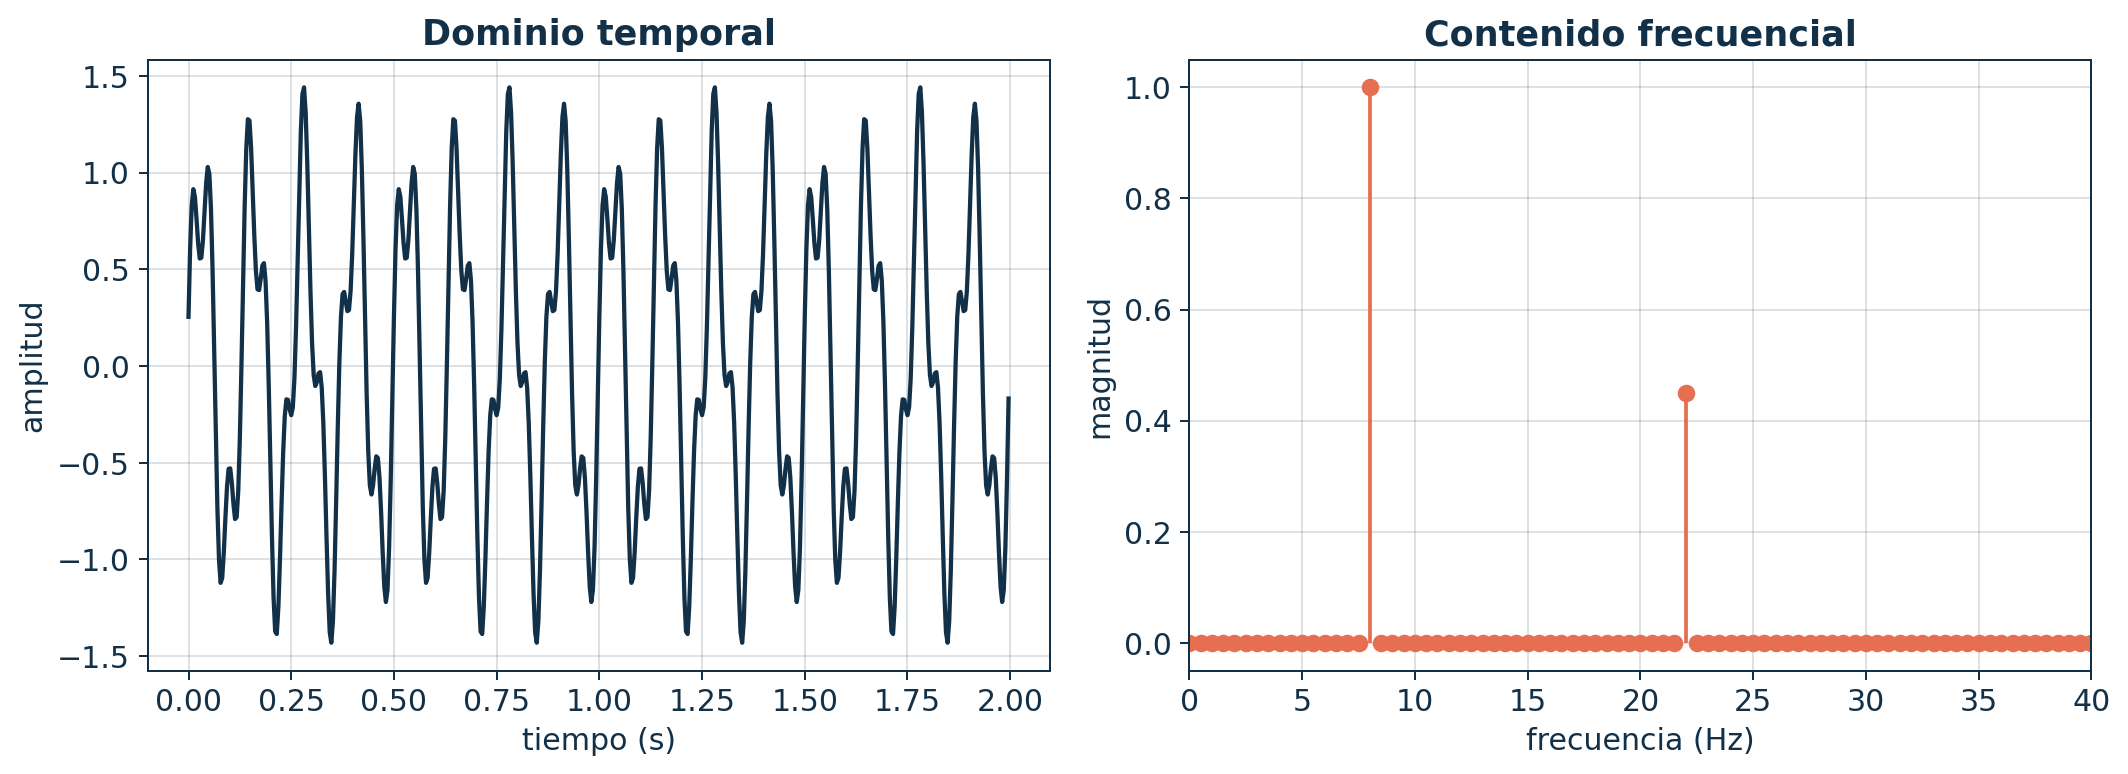
\includegraphics[width=0.84\linewidth,height=\textheight,keepaspectratio]{assets/17_time_frequency.png}

\begin{tcolorbox}[enhanced jigsaw, arc=.35mm, bottomrule=.15mm, bottomtitle=1mm, breakable, colback=white, colbacktitle=quarto-callout-important-color!10!white, colframe=quarto-callout-important-color-frame, coltitle=black, left=2mm, leftrule=.75mm, opacityback=0, opacitybacktitle=0.6, rightrule=.15mm, title={Cambio de perspectiva}, titlerule=0mm, toprule=.15mm, toptitle=1mm]

El dominio temporal conserva la localización de los eventos. El dominio
frecuencial reorganiza la señal según su contribución oscilatoria.

\end{tcolorbox}
\end{frame}

\begin{frame}{El dominio frecuencial responde preguntas específicas}
\protect\phantomsection\label{el-dominio-frecuencial-responde-preguntas-especuxedficas}
\begin{itemize}
\tightlist
\item
  ¿Qué oscilaciones contribuyen a la señal?
\item
  ¿Cuál componente tiene mayor magnitud?
\item
  ¿Qué ancho de banda ocupa el registro?
\item
  ¿Existen interferencias concentradas en frecuencias particulares?
\item
  ¿Cómo modifica un sistema cada componente?
\end{itemize}

\begin{tcolorbox}[enhanced jigsaw, arc=.35mm, bottomrule=.15mm, bottomtitle=1mm, breakable, colback=white, colbacktitle=quarto-callout-warning-color!10!white, colframe=quarto-callout-warning-color-frame, coltitle=black, left=2mm, leftrule=.75mm, opacityback=0, opacitybacktitle=0.6, rightrule=.15mm, title={No es una vista superior}, titlerule=0mm, toprule=.15mm, toptitle=1mm]

Tiempo y frecuencia son representaciones complementarias. El espectro
global puede ocultar cuándo ocurrió un cambio.

\end{tcolorbox}
\end{frame}

\begin{frame}{Sumar componentes simples produce formas complejas}
\protect\phantomsection\label{sumar-componentes-simples-produce-formas-complejas}
Considere

\[
x(t)=A_1\cos(2\pi f_1t+\phi_1)
+A_2\cos(2\pi f_2t+\phi_2).
\]

La forma temporal resulta de la interferencia constructiva y destructiva
entre componentes.

\begin{tcolorbox}[enhanced jigsaw, arc=.35mm, bottomrule=.15mm, bottomtitle=1mm, breakable, colback=white, colbacktitle=quarto-callout-note-color!10!white, colframe=quarto-callout-note-color-frame, coltitle=black, left=2mm, leftrule=.75mm, opacityback=0, opacitybacktitle=0.6, rightrule=.15mm, title={Interpretación}, titlerule=0mm, toprule=.15mm, toptitle=1mm]

El análisis frecuencial busca estimar cuánto aporta cada función base a
la señal observada.

\end{tcolorbox}
\end{frame}

\begin{frame}{Una base permite describir un objeto mediante coordenadas}
\protect\phantomsection\label{una-base-permite-describir-un-objeto-mediante-coordenadas}
En un espacio vectorial:

\[
\mathbf{x}=c_1\mathbf{b}_1+c_2\mathbf{b}_2+\cdots+c_K\mathbf{b}_K.
\]

En señales, las funciones base reemplazan a los vectores geométricos:

\[
x(t)=\sum_k c_k\,\phi_k(t).
\]

\begin{tcolorbox}[enhanced jigsaw, arc=.35mm, bottomrule=.15mm, bottomtitle=1mm, breakable, colback=white, colbacktitle=quarto-callout-important-color!10!white, colframe=quarto-callout-important-color-frame, coltitle=black, left=2mm, leftrule=.75mm, opacityback=0, opacitybacktitle=0.6, rightrule=.15mm, title={Idea de Fourier}, titlerule=0mm, toprule=.15mm, toptitle=1mm]

Usamos sinusoides o exponenciales complejas como funciones base y
calculamos sus coeficientes.

\end{tcolorbox}
\end{frame}

\begin{frame}{Fórmula de Euler}
\protect\phantomsection\label{fuxf3rmula-de-euler}
\[
e^{j\alpha}=\cos\alpha+j\sin\alpha.
\]

De ella se obtiene:

\[
\cos\alpha=\frac{e^{j\alpha}+e^{-j\alpha}}{2},
\qquad
\sin\alpha=\frac{e^{j\alpha}-e^{-j\alpha}}{2j}.
\]

\begin{tcolorbox}[enhanced jigsaw, arc=.35mm, bottomrule=.15mm, bottomtitle=1mm, breakable, colback=white, colbacktitle=quarto-callout-note-color!10!white, colframe=quarto-callout-note-color-frame, coltitle=black, left=2mm, leftrule=.75mm, opacityback=0, opacitybacktitle=0.6, rightrule=.15mm, title={Utilidad}, titlerule=0mm, toprule=.15mm, toptitle=1mm]

Las exponenciales complejas simplifican derivación, integración y
análisis de sistemas lineales.

\end{tcolorbox}
\end{frame}

\begin{frame}[shrink]{La exponencial compleja es una rotación}
\protect\phantomsection\label{la-exponencial-compleja-es-una-rotaciuxf3n}
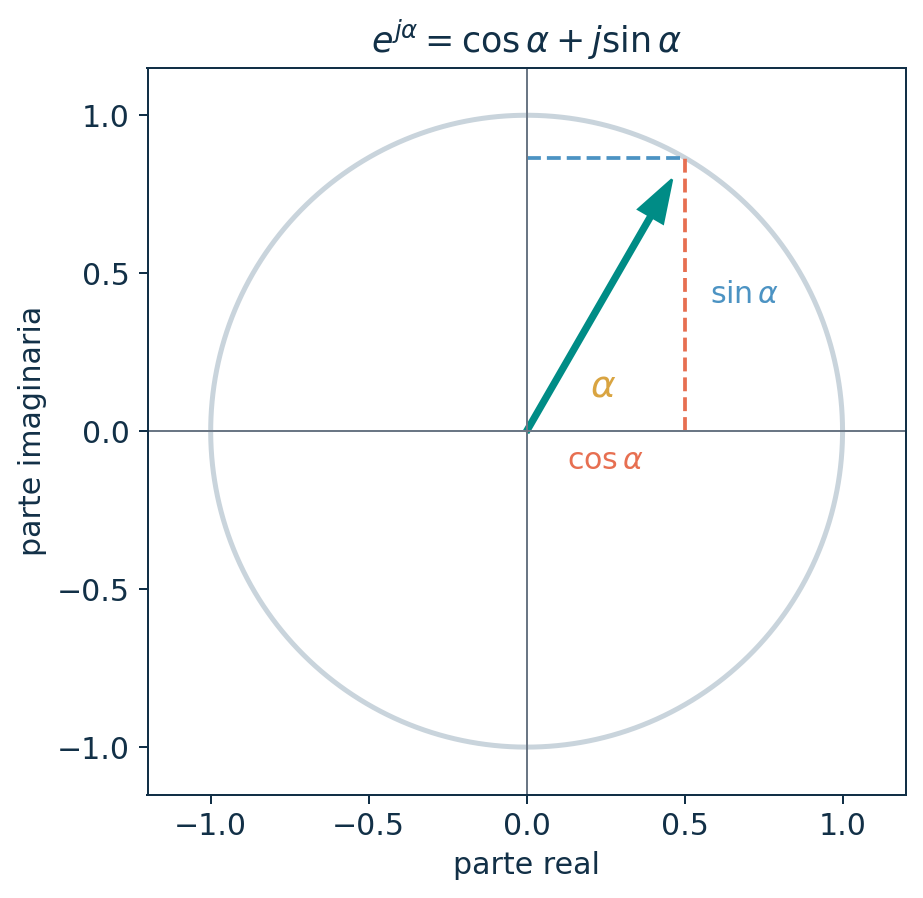
\includegraphics[width=0.5\linewidth,height=\textheight,keepaspectratio]{assets/18_complex_plane.png}

\begin{tcolorbox}[enhanced jigsaw, arc=.35mm, bottomrule=.15mm, bottomtitle=1mm, breakable, colback=white, colbacktitle=quarto-callout-tip-color!10!white, colframe=quarto-callout-tip-color-frame, coltitle=black, left=2mm, leftrule=.75mm, opacityback=0, opacitybacktitle=0.6, rightrule=.15mm, title={Lectura geométrica}, titlerule=0mm, toprule=.15mm, toptitle=1mm]

\(\cos\alpha\) es la proyección real y \(\sin\alpha\) la proyección
imaginaria de un punto sobre la circunferencia unitaria.

\end{tcolorbox}
\end{frame}

\begin{frame}{Exponenciales complejas y frecuencia}
\protect\phantomsection\label{exponenciales-complejas-y-frecuencia}
\[
e^{j\omega t}
\]

describe una rotación con velocidad angular \(\omega\).

\begin{itemize}
\tightlist
\item
  La parte real es \(\cos(\omega t)\).
\item
  La parte imaginaria es \(\sin(\omega t)\).
\item
  \(e^{-j\omega t}\) rota en dirección contraria.
\end{itemize}

\begin{tcolorbox}[enhanced jigsaw, arc=.35mm, bottomrule=.15mm, bottomtitle=1mm, breakable, colback=white, colbacktitle=quarto-callout-important-color!10!white, colframe=quarto-callout-important-color-frame, coltitle=black, left=2mm, leftrule=.75mm, opacityback=0, opacitybacktitle=0.6, rightrule=.15mm, title={Representación bilateral}, titlerule=0mm, toprule=.15mm, toptitle=1mm]

Una sinusoide real se expresa mediante componentes de frecuencia
positiva y negativa.

\end{tcolorbox}
\end{frame}

\begin{frame}{Producto interno entre señales}
\protect\phantomsection\label{producto-interno-entre-seuxf1ales}
Para funciones definidas en un periodo \(T_0\):

\[
\langle x,y\rangle
=\frac{1}{T_0}\int_{t_0}^{t_0+T_0}x(t)y^*(t)\,dt.
\]

Dos funciones son ortogonales cuando

\[\langle x,y\rangle=0.\]

\begin{tcolorbox}[enhanced jigsaw, arc=.35mm, bottomrule=.15mm, bottomtitle=1mm, breakable, colback=white, colbacktitle=quarto-callout-note-color!10!white, colframe=quarto-callout-note-color-frame, coltitle=black, left=2mm, leftrule=.75mm, opacityback=0, opacitybacktitle=0.6, rightrule=.15mm, title={Interpretación}, titlerule=0mm, toprule=.15mm, toptitle=1mm]

El producto interno cuantifica semejanza considerando fase y amplitud
sobre el intervalo definido.

\end{tcolorbox}
\end{frame}

\begin{frame}[shrink]{Las bases sinusoidales son ortogonales}
\protect\phantomsection\label{las-bases-sinusoidales-son-ortogonales}
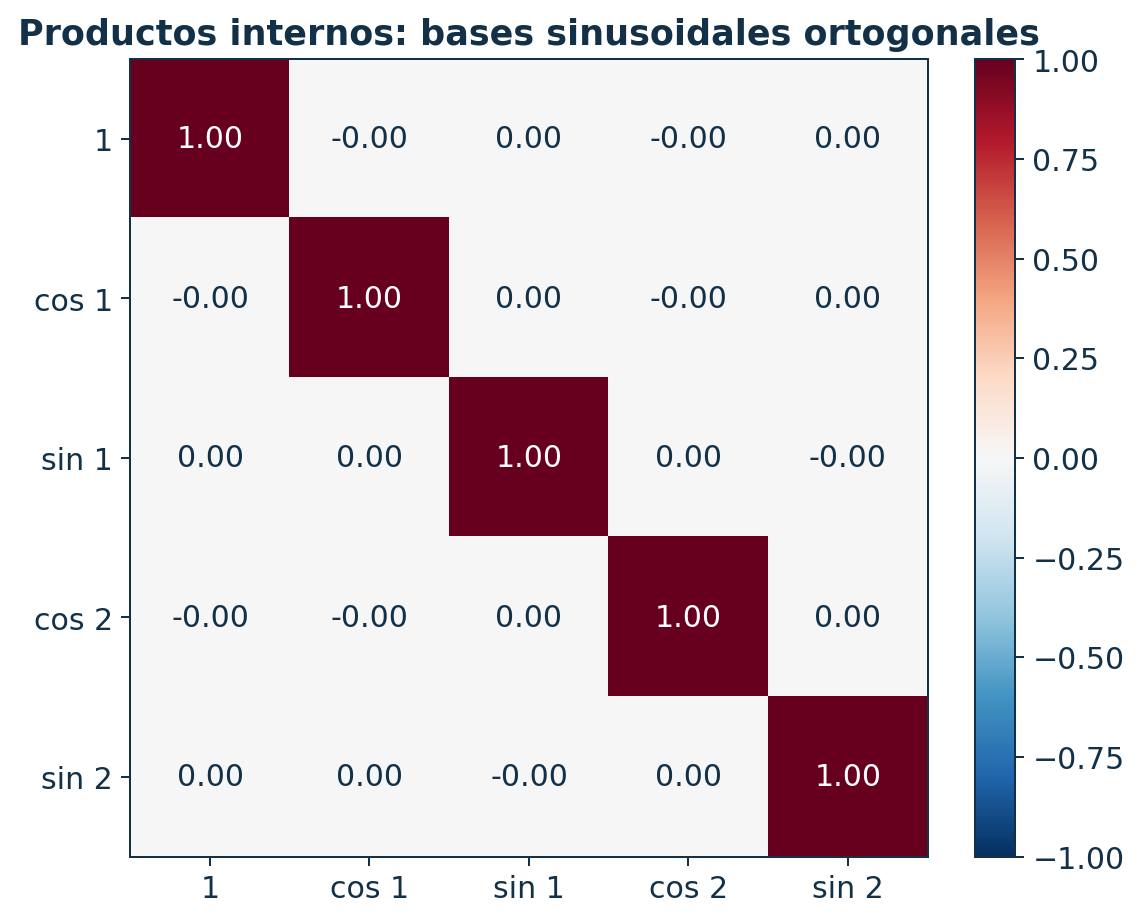
\includegraphics[width=0.55\linewidth,height=\textheight,keepaspectratio]{assets/19_orthogonality.png}

\begin{tcolorbox}[enhanced jigsaw, arc=.35mm, bottomrule=.15mm, bottomtitle=1mm, breakable, colback=white, colbacktitle=quarto-callout-important-color!10!white, colframe=quarto-callout-important-color-frame, coltitle=black, left=2mm, leftrule=.75mm, opacityback=0, opacitybacktitle=0.6, rightrule=.15mm, title={Consecuencia}, titlerule=0mm, toprule=.15mm, toptitle=1mm]

La ortogonalidad permite aislar un coeficiente sin que las demás
componentes contaminen su estimación ideal.

\end{tcolorbox}
\end{frame}

\begin{frame}{Coeficiente como proyección}
\protect\phantomsection\label{coeficiente-como-proyecciuxf3n}
Si las funciones \(\phi_k\) son ortonormales,

\[
c_k=\langle x,\phi_k\rangle.
\]

El coeficiente informa:

\begin{itemize}
\tightlist
\item
  cuánto de la base \(k\) está presente;
\item
  qué escala debe aplicarse;
\item
  qué fase relativa tiene la contribución.
\end{itemize}

\begin{tcolorbox}[enhanced jigsaw, arc=.35mm, bottomrule=.15mm, bottomtitle=1mm, breakable, colback=white, colbacktitle=quarto-callout-tip-color!10!white, colframe=quarto-callout-tip-color-frame, coltitle=black, left=2mm, leftrule=.75mm, opacityback=0, opacitybacktitle=0.6, rightrule=.15mm, title={Analogía}, titlerule=0mm, toprule=.15mm, toptitle=1mm]

Así como las coordenadas \((x,y)\) proyectan un vector sobre ejes
ortogonales, Fourier proyecta una señal sobre oscilaciones ortogonales.

\end{tcolorbox}
\end{frame}

\begin{frame}{Magnitud y fase contienen información diferente}
\protect\phantomsection\label{magnitud-y-fase-contienen-informaciuxf3n-diferente}
Para un coeficiente complejo \(C_k\):

\[
C_k=|C_k|e^{j\angle C_k}.
\]

\begin{itemize}
\tightlist
\item
  \(|C_k|\): magnitud de la contribución.
\item
  \(\angle C_k\): alineación o fase de esa contribución.
\end{itemize}

\begin{tcolorbox}[enhanced jigsaw, arc=.35mm, bottomrule=.15mm, bottomtitle=1mm, breakable, colback=white, colbacktitle=quarto-callout-warning-color!10!white, colframe=quarto-callout-warning-color-frame, coltitle=black, left=2mm, leftrule=.75mm, opacityback=0, opacitybacktitle=0.6, rightrule=.15mm, title={Error frecuente}, titlerule=0mm, toprule=.15mm, toptitle=1mm]

Conservar solo magnitud puede ser suficiente para algunas
características, pero no permite reconstruir en general la forma
temporal original.

\end{tcolorbox}
\end{frame}

\begin{frame}{Limitaciones del espectro global}
\protect\phantomsection\label{limitaciones-del-espectro-global}
El análisis global supone que el intervalo completo puede resumirse con
los mismos componentes.

Esto puede fallar cuando:

\begin{itemize}
\tightlist
\item
  la señal cambia de estado;
\item
  aparecen eventos breves;
\item
  la frecuencia dominante evoluciona;
\item
  las ventanas mezclan condiciones;
\item
  existen discontinuidades artificiales en los bordes.
\end{itemize}

\begin{tcolorbox}[enhanced jigsaw, arc=.35mm, bottomrule=.15mm, bottomtitle=1mm, breakable, colback=white, colbacktitle=quarto-callout-caution-color!10!white, colframe=quarto-callout-caution-color-frame, coltitle=black, left=2mm, leftrule=.75mm, opacityback=0, opacitybacktitle=0.6, rightrule=.15mm, title={Señales biomédicas}, titlerule=0mm, toprule=.15mm, toptitle=1mm]

Muchas bioseñales son localmente estacionarias solo durante intervalos
limitados. La segmentación precede al análisis espectral.

\end{tcolorbox}
\end{frame}

\begin{frame}{Actividad: tiempo, frecuencia o ambas}
\protect\phantomsection\label{actividad-tiempo-frecuencia-o-ambas}
Seleccione la representación más informativa y justifique:

\begin{enumerate}
\tightlist
\item
  medir la latencia entre dos eventos;
\item
  identificar una interferencia sinusoidal;
\item
  estudiar una oscilación que aparece durante un segundo;
\item
  comparar la amplitud de dos contracciones;
\item
  describir una señal con componentes simultáneas.
\end{enumerate}

\begin{tcolorbox}[enhanced jigsaw, arc=.35mm, bottomrule=.15mm, bottomtitle=1mm, breakable, colback=white, colbacktitle=quarto-callout-note-color!10!white, colframe=quarto-callout-note-color-frame, coltitle=black, left=2mm, leftrule=.75mm, opacityback=0, opacitybacktitle=0.6, rightrule=.15mm, title={Criterio}, titlerule=0mm, toprule=.15mm, toptitle=1mm]

No se busca una etiqueta aislada. La justificación debe indicar qué
información conserva y qué información pierde cada representación.

\end{tcolorbox}
\end{frame}

\begin{frame}{Cierre de la sesión 9}
\protect\phantomsection\label{cierre-de-la-sesiuxf3n-9}
\begin{tcolorbox}[enhanced jigsaw, arc=.35mm, bottomrule=.15mm, bottomtitle=1mm, breakable, colback=white, colbacktitle=quarto-callout-important-color!10!white, colframe=quarto-callout-important-color-frame, coltitle=black, left=2mm, leftrule=.75mm, opacityback=0, opacitybacktitle=0.6, rightrule=.15mm, title={Síntesis}, titlerule=0mm, toprule=.15mm, toptitle=1mm]

Fourier interpreta una señal mediante proyecciones sobre bases
oscilatorias ortogonales. Los coeficientes complejos reúnen magnitud y
fase; el espectro complementa, pero no reemplaza, al tiempo.

\end{tcolorbox}

\textbf{Conexión:} aplicaremos estas ideas a señales periódicas mediante
la serie de Fourier.
\end{frame}

\section{Semana 5 · Sesión 2}\label{semana-5-sesiuxf3n-2}

\begin{frame}{La serie de Fourier representa señales periódicas}
\protect\phantomsection\label{la-serie-de-fourier-representa-seuxf1ales-periuxf3dicas}
Al finalizar esta sesión podrá:

\begin{itemize}
\tightlist
\item
  escribir la serie compleja de Fourier;
\item
  interpretar sus coeficientes;
\item
  relacionar simetría y reducción de términos;
\item
  reconstruir una señal mediante sumas parciales;
\item
  explicar el fenómeno de Gibbs y Parseval.
\end{itemize}

\begin{tcolorbox}[enhanced jigsaw, arc=.35mm, bottomrule=.15mm, bottomtitle=1mm, breakable, colback=white, colbacktitle=quarto-callout-note-color!10!white, colframe=quarto-callout-note-color-frame, coltitle=black, left=2mm, leftrule=.75mm, opacityback=0, opacitybacktitle=0.6, rightrule=.15mm, title={Pregunta inicial}, titlerule=0mm, toprule=.15mm, toptitle=1mm]

¿Cómo puede una suma de funciones suaves aproximar una señal con
discontinuidades?

\end{tcolorbox}
\end{frame}

\begin{frame}{Serie compleja de Fourier}
\protect\phantomsection\label{serie-compleja-de-fourier}
Para una señal periódica de periodo \(T_0\) y frecuencia angular
fundamental \(\omega_0=2\pi/T_0\):

\[
x(t)=\sum_{k=-\infty}^{\infty}C_k e^{jk\omega_0t}.
\]

Los coeficientes son

\[
C_k=\frac{1}{T_0}\int_{t_0}^{t_0+T_0}
x(t)e^{-jk\omega_0t}\,dt.
\]

\begin{tcolorbox}[enhanced jigsaw, arc=.35mm, bottomrule=.15mm, bottomtitle=1mm, breakable, colback=white, colbacktitle=quarto-callout-important-color!10!white, colframe=quarto-callout-important-color-frame, coltitle=black, left=2mm, leftrule=.75mm, opacityback=0, opacitybacktitle=0.6, rightrule=.15mm, title={Significado}, titlerule=0mm, toprule=.15mm, toptitle=1mm]

\(C_k\) es la coordenada compleja de \(x(t)\) asociada con el armónico
\(k\).

\end{tcolorbox}
\end{frame}

\begin{frame}{¿Qué representa el índice armónico?}
\protect\phantomsection\label{quuxe9-representa-el-uxedndice-armuxf3nico}
\begin{itemize}
\tightlist
\item
  \(k=0\): componente continua o valor medio.
\item
  \(k=\pm1\): frecuencia fundamental.
\item
  \(k=\pm2\): segundo armónico.
\item
  \(k=\pm3\): tercer armónico.
\item
  En general, el armónico \(k\) tiene frecuencia \(k f_0\).
\end{itemize}

\begin{tcolorbox}[enhanced jigsaw, arc=.35mm, bottomrule=.15mm, bottomtitle=1mm, breakable, colback=white, colbacktitle=quarto-callout-note-color!10!white, colframe=quarto-callout-note-color-frame, coltitle=black, left=2mm, leftrule=.75mm, opacityback=0, opacitybacktitle=0.6, rightrule=.15mm, title={Espectro de líneas}, titlerule=0mm, toprule=.15mm, toptitle=1mm]

Una señal periódica ideal posee componentes en múltiplos enteros de la
frecuencia fundamental.

\end{tcolorbox}
\end{frame}

\begin{frame}{Forma trigonométrica}
\protect\phantomsection\label{forma-trigonomuxe9trica}
Una representación real equivalente es

\[
x(t)=\frac{a_0}{2}
+\sum_{k=1}^{\infty}
\left[a_k\cos(k\omega_0t)+b_k\sin(k\omega_0t)\right].
\]

Los coeficientes \(a_k\) y \(b_k\) expresan contribuciones cosenoidales
y sinusoidales.

\begin{tcolorbox}[enhanced jigsaw, arc=.35mm, bottomrule=.15mm, bottomtitle=1mm, breakable, colback=white, colbacktitle=quarto-callout-tip-color!10!white, colframe=quarto-callout-tip-color-frame, coltitle=black, left=2mm, leftrule=.75mm, opacityback=0, opacitybacktitle=0.6, rightrule=.15mm, title={Elección de forma}, titlerule=0mm, toprule=.15mm, toptitle=1mm]

La forma trigonométrica facilita visualizar senos y cosenos; la compleja
simplifica operaciones algebraicas.

\end{tcolorbox}
\end{frame}

\begin{frame}{Las simetrías reducen el cálculo}
\protect\phantomsection\label{las-simetruxedas-reducen-el-cuxe1lculo}
Para un intervalo simétrico:

\begin{itemize}
\tightlist
\item
  si \(x(t)\) es par, los términos sinusoidales se anulan: \(b_k=0\);
\item
  si \(x(t)\) es impar, los términos cosenoidales y el promedio se
  anulan: \(a_k=0\) y \(a_0=0\);
\item
  otras simetrías pueden eliminar armónicos pares o impares.
\end{itemize}

\begin{tcolorbox}[enhanced jigsaw, arc=.35mm, bottomrule=.15mm, bottomtitle=1mm, breakable, colback=white, colbacktitle=quarto-callout-important-color!10!white, colframe=quarto-callout-important-color-frame, coltitle=black, left=2mm, leftrule=.75mm, opacityback=0, opacitybacktitle=0.6, rightrule=.15mm, title={Antes de integrar}, titlerule=0mm, toprule=.15mm, toptitle=1mm]

Inspeccione periodicidad y simetrías. Pueden reducir sustancialmente el
número de cálculos.

\end{tcolorbox}
\end{frame}

\begin{frame}{Ejemplo: onda cuadrada impar}
\protect\phantomsection\label{ejemplo-onda-cuadrada-impar}
Para una onda cuadrada ideal de amplitud \(\pm1\) y periodo \(2\pi\):

\[
x(t)=\frac{4}{\pi}
\sum_{m=0}^{\infty}
\frac{\sin\big((2m+1)t\big)}{2m+1}.
\]

\begin{tcolorbox}[enhanced jigsaw, arc=.35mm, bottomrule=.15mm, bottomtitle=1mm, breakable, colback=white, colbacktitle=quarto-callout-note-color!10!white, colframe=quarto-callout-note-color-frame, coltitle=black, left=2mm, leftrule=.75mm, opacityback=0, opacitybacktitle=0.6, rightrule=.15mm, title={Estructura}, titlerule=0mm, toprule=.15mm, toptitle=1mm]

Solo aparecen armónicos impares y su amplitud decrece de manera
inversamente proporcional al índice.

\end{tcolorbox}
\end{frame}

\begin{frame}[shrink]{Reconstrucción mediante sumas parciales}
\protect\phantomsection\label{reconstrucciuxf3n-mediante-sumas-parciales}
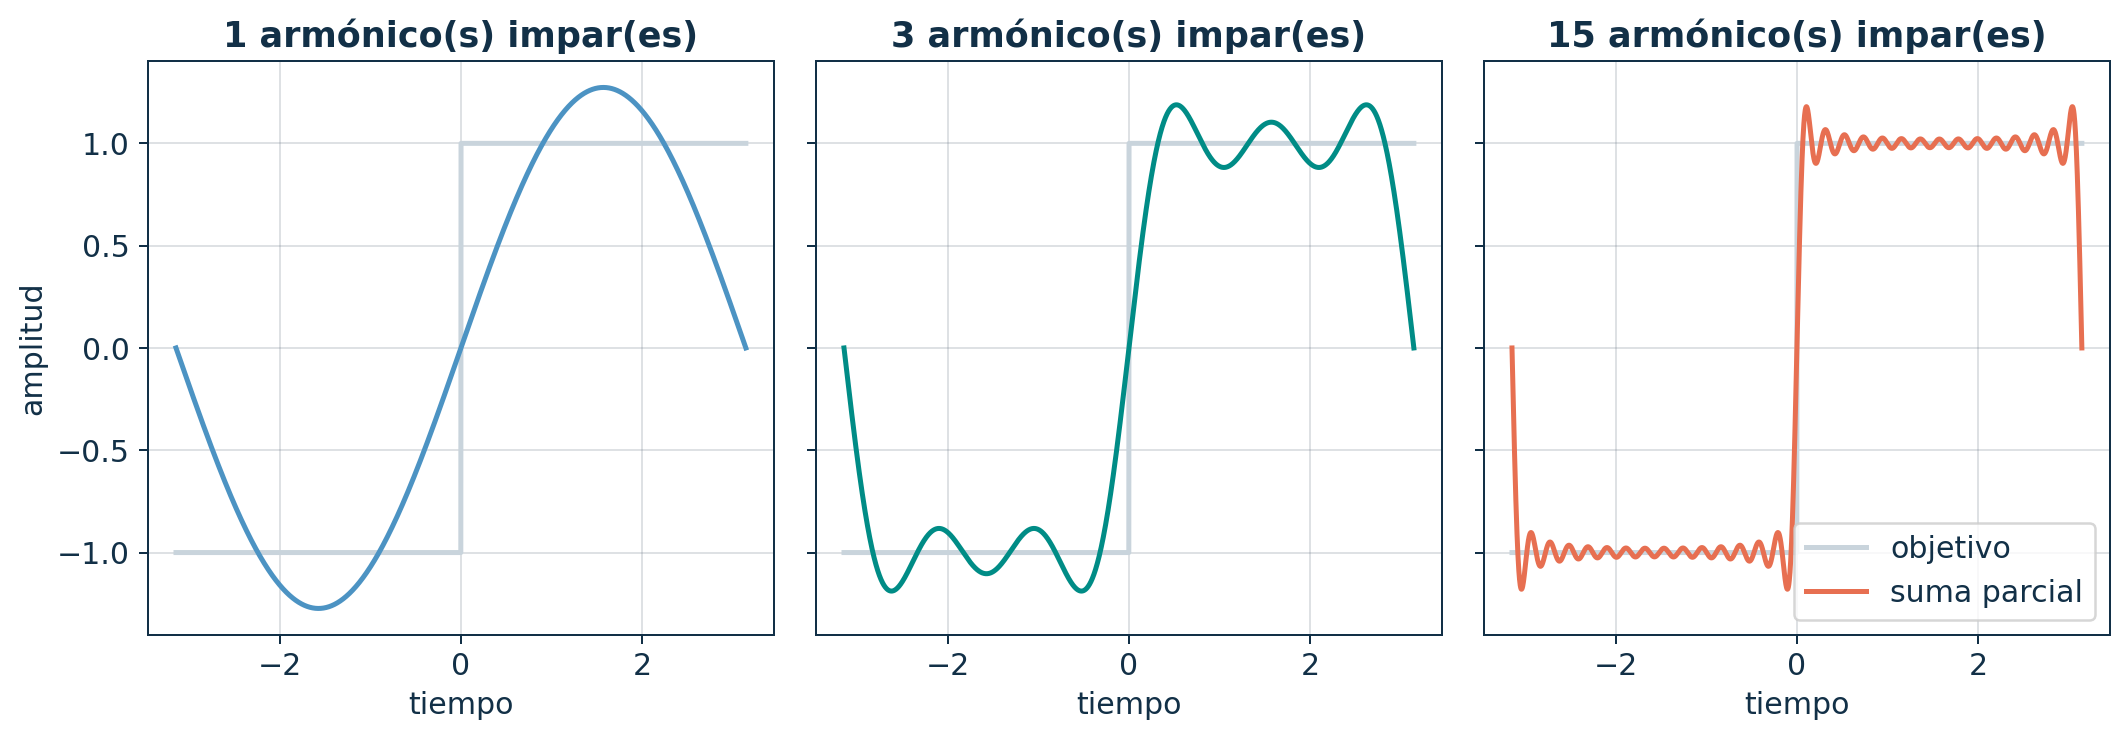
\includegraphics[width=0.85\linewidth,height=\textheight,keepaspectratio]{assets/20_fourier_square.png}

\begin{tcolorbox}[enhanced jigsaw, arc=.35mm, bottomrule=.15mm, bottomtitle=1mm, breakable, colback=white, colbacktitle=quarto-callout-important-color!10!white, colframe=quarto-callout-important-color-frame, coltitle=black, left=2mm, leftrule=.75mm, opacityback=0, opacitybacktitle=0.6, rightrule=.15mm, title={Lectura}, titlerule=0mm, toprule=.15mm, toptitle=1mm]

Al añadir armónicos se recuperan bordes más rápidos y regiones más
planas. La reconstrucción sigue siendo continua para cualquier número
finito de términos.

\end{tcolorbox}
\end{frame}

\begin{frame}[shrink]{Fenómeno de Gibbs}
\protect\phantomsection\label{fenuxf3meno-de-gibbs}
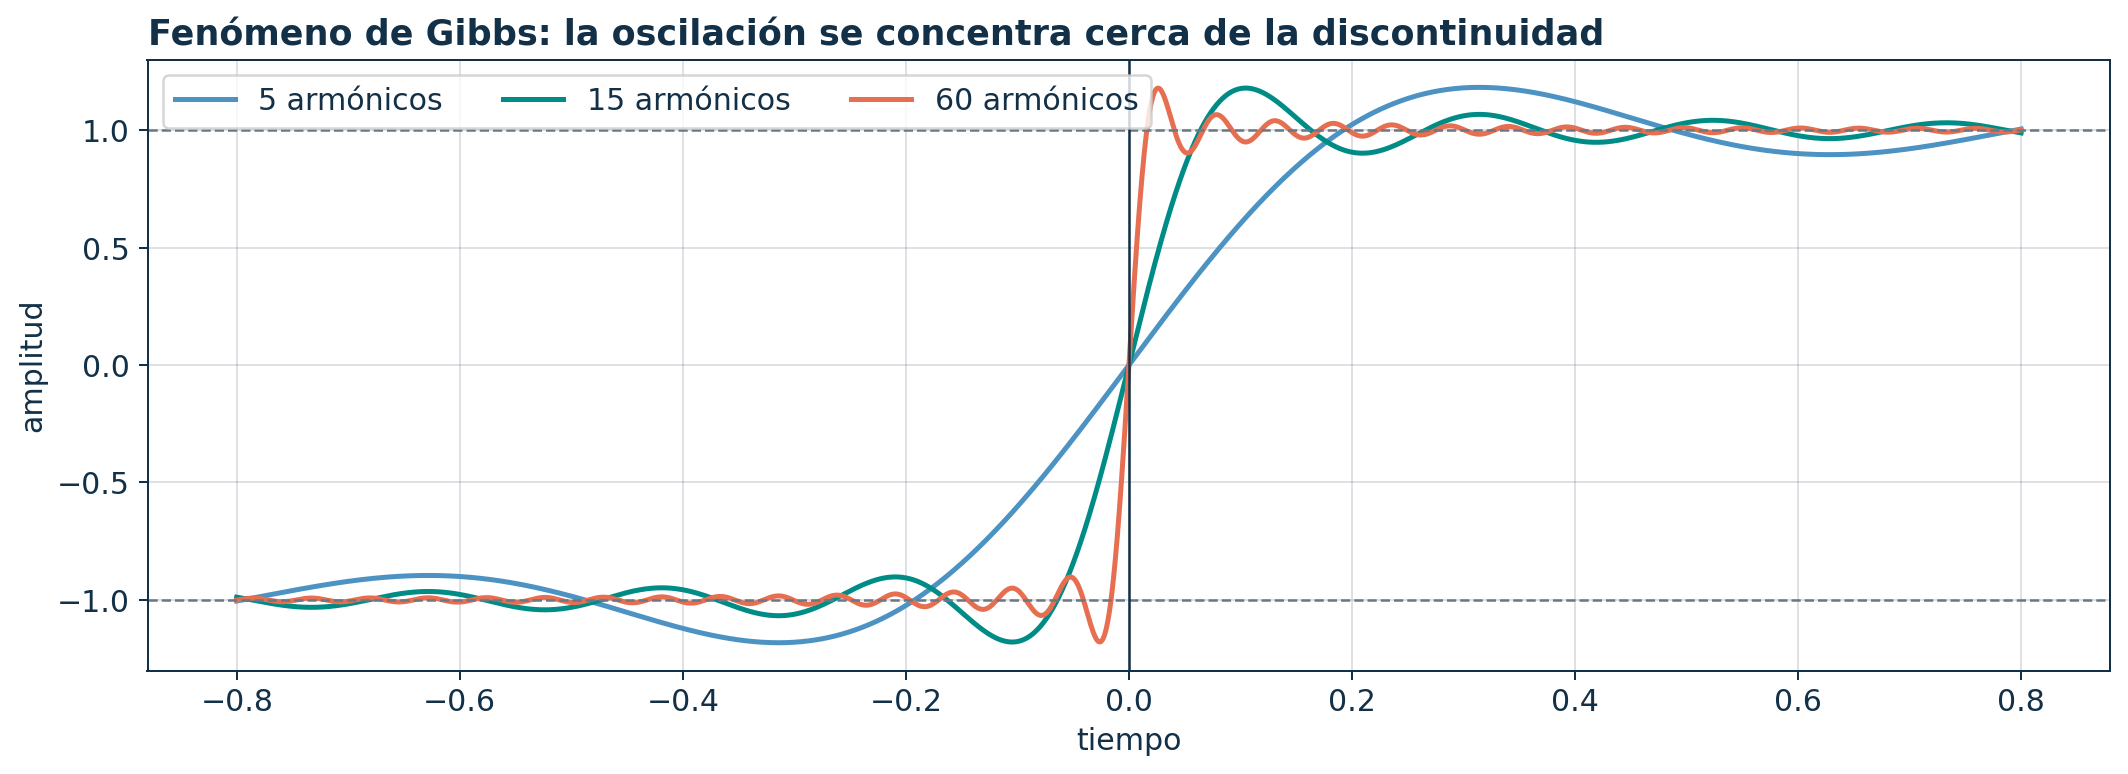
\includegraphics[width=0.83\linewidth,height=\textheight,keepaspectratio]{assets/21_gibbs.png}

\begin{tcolorbox}[enhanced jigsaw, arc=.35mm, bottomrule=.15mm, bottomtitle=1mm, breakable, colback=white, colbacktitle=quarto-callout-warning-color!10!white, colframe=quarto-callout-warning-color-frame, coltitle=black, left=2mm, leftrule=.75mm, opacityback=0, opacitybacktitle=0.6, rightrule=.15mm, title={Concepto principal}, titlerule=0mm, toprule=.15mm, toptitle=1mm]

Al aumentar el número de armónicos, la oscilación se concentra cerca de
la discontinuidad, pero el sobreimpulso no desaparece simplemente en
altura.

\end{tcolorbox}
\end{frame}

\begin{frame}{Convergencia en una discontinuidad}
\protect\phantomsection\label{convergencia-en-una-discontinuidad}
En condiciones habituales, la serie converge en un salto al promedio
lateral:

\[
\lim_{N\to\infty}x_N(t_d)
=\frac{x(t_d^-)+x(t_d^+)}{2}.
\]

\begin{tcolorbox}[enhanced jigsaw, arc=.35mm, bottomrule=.15mm, bottomtitle=1mm, breakable, colback=white, colbacktitle=quarto-callout-note-color!10!white, colframe=quarto-callout-note-color-frame, coltitle=black, left=2mm, leftrule=.75mm, opacityback=0, opacitybacktitle=0.6, rightrule=.15mm, title={Interpretación}, titlerule=0mm, toprule=.15mm, toptitle=1mm]

La representación de Fourier aproxima la señal en un sentido global; no
obliga a que cada punto discontinuo adopte uno de sus valores laterales.

\end{tcolorbox}
\end{frame}

\begin{frame}{Parseval conecta potencia temporal y coeficientes}
\protect\phantomsection\label{parseval-conecta-potencia-temporal-y-coeficientes}
Para la serie compleja:

\[
\frac{1}{T_0}\int_{t_0}^{t_0+T_0}|x(t)|^2dt
=\sum_{k=-\infty}^{\infty}|C_k|^2.
\]

\begin{tcolorbox}[enhanced jigsaw, arc=.35mm, bottomrule=.15mm, bottomtitle=1mm, breakable, colback=white, colbacktitle=quarto-callout-important-color!10!white, colframe=quarto-callout-important-color-frame, coltitle=black, left=2mm, leftrule=.75mm, opacityback=0, opacitybacktitle=0.6, rightrule=.15mm, title={Conservación}, titlerule=0mm, toprule=.15mm, toptitle=1mm]

La potencia promedio calculada en el tiempo coincide con la suma de las
contribuciones cuadráticas de los armónicos.

\end{tcolorbox}
\end{frame}

\begin{frame}[fragile]{Reconstrucción en Python}
\protect\phantomsection\label{reconstrucciuxf3n-en-python}
\begin{Shaded}
\begin{Highlighting}[]
\ImportTok{import}\NormalTok{ numpy }\ImportTok{as}\NormalTok{ np}

\NormalTok{t }\OperatorTok{=}\NormalTok{ np.linspace(}\OperatorTok{{-}}\NormalTok{np.pi, np.pi, }\DecValTok{2000}\NormalTok{)}
\NormalTok{xN }\OperatorTok{=}\NormalTok{ np.zeros\_like(t)}

\NormalTok{terms }\OperatorTok{=} \DecValTok{15}
\ControlFlowTok{for}\NormalTok{ m }\KeywordTok{in} \BuiltInTok{range}\NormalTok{(terms):}
\NormalTok{    k }\OperatorTok{=} \DecValTok{2}\OperatorTok{*}\NormalTok{m }\OperatorTok{+} \DecValTok{1}
\NormalTok{    xN }\OperatorTok{+=}\NormalTok{ (}\DecValTok{4}\OperatorTok{/}\NormalTok{np.pi) }\OperatorTok{*}\NormalTok{ np.sin(k}\OperatorTok{*}\NormalTok{t) }\OperatorTok{/}\NormalTok{ k}
\end{Highlighting}
\end{Shaded}

\begin{tcolorbox}[enhanced jigsaw, arc=.35mm, bottomrule=.15mm, bottomtitle=1mm, breakable, colback=white, colbacktitle=quarto-callout-tip-color!10!white, colframe=quarto-callout-tip-color-frame, coltitle=black, left=2mm, leftrule=.75mm, opacityback=0, opacitybacktitle=0.6, rightrule=.15mm, title={Experimento}, titlerule=0mm, toprule=.15mm, toptitle=1mm]

Cambie \texttt{terms} y observe qué regiones mejoran, dónde persisten
oscilaciones y cómo cambia el error global.

\end{tcolorbox}
\end{frame}

\begin{frame}{No confunda serie, transformada y DFT}
\protect\phantomsection\label{no-confunda-serie-transformada-y-dft}
{\def\LTcaptype{none} % do not increment counter
\begin{longtable}[]{@{}
  >{\raggedright\arraybackslash}p{(\linewidth - 4\tabcolsep) * \real{0.3333}}
  >{\raggedright\arraybackslash}p{(\linewidth - 4\tabcolsep) * \real{0.3333}}
  >{\raggedright\arraybackslash}p{(\linewidth - 4\tabcolsep) * \real{0.3333}}@{}}
\toprule\noalign{}
\begin{minipage}[b]{\linewidth}\raggedright
Herramienta
\end{minipage} & \begin{minipage}[b]{\linewidth}\raggedright
Señal idealizada
\end{minipage} & \begin{minipage}[b]{\linewidth}\raggedright
Resultado
\end{minipage} \\
\midrule\noalign{}
\endhead
Serie de Fourier & periódica continua & coeficientes discretos en
frecuencia \\
Transformada de Fourier & aperiódica continua & función continua de
frecuencia \\
DTFT & secuencia discreta & función periódica y continua en
frecuencia \\
DFT & bloque finito de muestras & conjunto finito de coeficientes \\
\bottomrule\noalign{}
\end{longtable}
}

\begin{tcolorbox}[enhanced jigsaw, arc=.35mm, bottomrule=.15mm, bottomtitle=1mm, breakable, colback=white, colbacktitle=quarto-callout-warning-color!10!white, colframe=quarto-callout-warning-color-frame, coltitle=black, left=2mm, leftrule=.75mm, opacityback=0, opacitybacktitle=0.6, rightrule=.15mm, title={Alcance de estas semanas}, titlerule=0mm, toprule=.15mm, toptitle=1mm]

En esta sesión se introduce la serie de Fourier. La transformada y la
DFT requieren desarrollar con cuidado muestreo, ventanas y resolución
frecuencial.

\end{tcolorbox}
\end{frame}

\begin{frame}{Aplicación biomédica: interpretar componentes, no
etiquetas}
\protect\phantomsection\label{aplicaciuxf3n-biomuxe9dica-interpretar-componentes-no-etiquetas}
El contenido armónico puede reflejar:

\begin{itemize}
\tightlist
\item
  repetición morfológica;
\item
  oscilaciones fisiológicas;
\item
  interferencia periódica;
\item
  bordes o transitorios;
\item
  efectos del sensor y del acondicionamiento.
\end{itemize}

\begin{tcolorbox}[enhanced jigsaw, arc=.35mm, bottomrule=.15mm, bottomtitle=1mm, breakable, colback=white, colbacktitle=quarto-callout-caution-color!10!white, colframe=quarto-callout-caution-color-frame, coltitle=black, left=2mm, leftrule=.75mm, opacityback=0, opacitybacktitle=0.6, rightrule=.15mm, title={Razonamiento crítico}, titlerule=0mm, toprule=.15mm, toptitle=1mm]

Encontrar una componente frecuencial no identifica automáticamente su
causa. La atribución exige contexto fisiológico, instrumental y
experimental.

\end{tcolorbox}
\end{frame}

\begin{frame}{Actividad de cierre}
\protect\phantomsection\label{actividad-de-cierre}
Una señal periódica es impar y presenta simetría de media onda.

\begin{enumerate}
\tightlist
\item
  ¿Qué familias de coeficientes podrían anularse?
\item
  ¿Qué información debe verificarse antes de calcular la serie?
\item
  ¿Qué ocurre en una discontinuidad durante la reconstrucción?
\item
  ¿Cómo comprobaría numéricamente la relación de Parseval?
\end{enumerate}

\begin{tcolorbox}[enhanced jigsaw, arc=.35mm, bottomrule=.15mm, bottomtitle=1mm, breakable, colback=white, colbacktitle=quarto-callout-tip-color!10!white, colframe=quarto-callout-tip-color-frame, coltitle=black, left=2mm, leftrule=.75mm, opacityback=0, opacitybacktitle=0.6, rightrule=.15mm, title={Criterio de respuesta}, titlerule=0mm, toprule=.15mm, toptitle=1mm]

Use simetrías para formular hipótesis, pero demuestre qué términos se
anulan mediante las definiciones.

\end{tcolorbox}
\end{frame}

\begin{frame}{Integración de las semanas 1--5}
\protect\phantomsection\label{integraciuxf3n-de-las-semanas-15}
\begin{tcolorbox}[enhanced jigsaw, arc=.35mm, bottomrule=.15mm, bottomtitle=1mm, breakable, colback=white, colbacktitle=quarto-callout-important-color!10!white, colframe=quarto-callout-important-color-frame, coltitle=black, left=2mm, leftrule=.75mm, opacityback=0, opacitybacktitle=0.6, rightrule=.15mm, title={Cadena conceptual}, titlerule=0mm, toprule=.15mm, toptitle=1mm]

\textbf{Fisiología y contexto} definen la pregunta → la
\textbf{medición} produce un registro → la \textbf{representación}
organiza los datos → la \textbf{segmentación} define observaciones → las
\textbf{características temporales o frecuenciales} construyen
evidencia.

\end{tcolorbox}

Ningún paso es neutral: cada elección determina qué información se
conserva, se transforma o se pierde.
\end{frame}

\begin{frame}{Preguntas de verificación acumulativa}
\protect\phantomsection\label{preguntas-de-verificaciuxf3n-acumulativa}
\begin{enumerate}
\tightlist
\item
  ¿Por qué una señal no puede interpretarse sin metadatos?
\item
  ¿Cuándo RMS y desviación estándar son iguales?
\item
  ¿Qué condición hace periódica una sinusoide discreta?
\item
  ¿Cómo se interpreta \(x(at-b)\) sin cometer errores de signo?
\item
  ¿Por qué las ventanas solapadas no son independientes?
\item
  ¿Qué representa un coeficiente de Fourier?
\item
  ¿Qué información se pierde al conservar solo la magnitud espectral?
\end{enumerate}
\end{frame}

\begin{frame}{Criterios de aprendizaje alcanzados}
\protect\phantomsection\label{criterios-de-aprendizaje-alcanzados}
Al completar estas semanas, el estudiante debe poder:

\begin{itemize}
\tightlist
\item
  formular una pregunta de análisis conectada con fisiología y
  adquisición;
\item
  representar señales escalares y multicanal con unidades;
\item
  calcular e interpretar características temporales;
\item
  demostrar periodicidad y ejecutar transformaciones;
\item
  construir un flujo temporal reproducible;
\item
  explicar Fourier como proyección sobre bases ortogonales;
\item
  reconocer límites metodológicos y evitar inferencias clínicas no
  justificadas.
\end{itemize}

\begin{tcolorbox}[enhanced jigsaw, arc=.35mm, bottomrule=.15mm, bottomtitle=1mm, breakable, colback=white, colbacktitle=quarto-callout-note-color!10!white, colframe=quarto-callout-note-color-frame, coltitle=black, left=2mm, leftrule=.75mm, opacityback=0, opacitybacktitle=0.6, rightrule=.15mm, title={Siguiente etapa}, titlerule=0mm, toprule=.15mm, toptitle=1mm]

Las semanas posteriores desarrollarán adquisición digital, espectros de
potencia, transformada discreta, sistemas lineales y filtrado.

\end{tcolorbox}
\end{frame}

\begin{frame}[shrink]{Referencias principales}
\protect\phantomsection\label{referencias-principales}
\protect\phantomsection\label{refs}
\begin{CSLReferences}{1}{1}
\bibitem[\citeproctext]{ref-esakkirajan2024}
Esakkirajan, S., T. Veerakumar, y Badri N. Subudhi. 2024. \emph{Digital
Signal Processing: Illustration Using Python}. Springer.
\url{https://doi.org/10.1007/978-981-99-6752-0}.

\bibitem[\citeproctext]{ref-kaniusas2012}
Kaniusas, Eugenijus. 2012. \emph{Biomedical Signals and Sensors I:
Linking Physiological Phenomena and Biosignals}. Springer.
\url{https://doi.org/10.1007/978-3-642-24843-6}.

\bibitem[\citeproctext]{ref-naik2024}
Naik, Ganesh R., y Wellington Pinheiro dos Santos, eds. 2024.
\emph{Biomedical Signal Processing: A Modern Approach}. CRC Press.
\url{https://doi.org/10.1201/9781003201137}.

\bibitem[\citeproctext]{ref-semmlow2014}
Semmlow, John L., y Benjamin Griffel. 2014. \emph{Biosignal and Medical
Image Processing}. 3.ª ed. CRC Press.

\end{CSLReferences}
\end{frame}

\begin{frame}[fragile]{Apéndice: entorno Python recomendado}
\protect\phantomsection\label{apuxe9ndice-entorno-python-recomendado}
\begin{Shaded}
\begin{Highlighting}[]
\ExtensionTok{uv}\NormalTok{ init sysb}
\BuiltInTok{cd}\NormalTok{ sysb}
\ExtensionTok{uv}\NormalTok{ add numpy scipy matplotlib pandas jupyter}
\ExtensionTok{uv}\NormalTok{ run jupyter lab}
\end{Highlighting}
\end{Shaded}

Bibliotecas principales:

\begin{itemize}
\tightlist
\item
  \texttt{NumPy}: arreglos y operaciones numéricas.
\item
  \texttt{SciPy.signal}: procesamiento de señales.
\item
  \texttt{Matplotlib}: visualización científica.
\item
  \texttt{Pandas}: tablas de características y metadatos.
\end{itemize}

\begin{tcolorbox}[enhanced jigsaw, arc=.35mm, bottomrule=.15mm, bottomtitle=1mm, breakable, colback=white, colbacktitle=quarto-callout-tip-color!10!white, colframe=quarto-callout-tip-color-frame, coltitle=black, left=2mm, leftrule=.75mm, opacityback=0, opacitybacktitle=0.6, rightrule=.15mm, title={Reproducibilidad}, titlerule=0mm, toprule=.15mm, toptitle=1mm]

Registre versiones del entorno y use una semilla explícita cuando genere
señales o ruido aleatorio.

\end{tcolorbox}
\end{frame}

\begin{frame}{Apéndice: plantilla mínima de una práctica}
\protect\phantomsection\label{apuxe9ndice-plantilla-muxednima-de-una-pruxe1ctica}
\begin{enumerate}
\tightlist
\item
  \textbf{Pregunta:} qué se desea medir o comparar.
\item
  \textbf{Datos:} señal, unidades, canales, \(f_s\) y condición.
\item
  \textbf{Calidad:} inspección, exclusiones y artefactos.
\item
  \textbf{Método:} ecuaciones, parámetros y código.
\item
  \textbf{Resultado:} figura o tabla sin valores inventados.
\item
  \textbf{Interpretación:} vínculo con fisiología.
\item
  \textbf{Limitaciones:} alternativas y sensibilidad.
\end{enumerate}

\begin{tcolorbox}[enhanced jigsaw, arc=.35mm, bottomrule=.15mm, bottomtitle=1mm, breakable, colback=white, colbacktitle=quarto-callout-important-color!10!white, colframe=quarto-callout-important-color-frame, coltitle=black, left=2mm, leftrule=.75mm, opacityback=0, opacitybacktitle=0.6, rightrule=.15mm, title={Estándar esperado}, titlerule=0mm, toprule=.15mm, toptitle=1mm]

El código ejecutable es necesario, pero no suficiente: una práctica
válida debe justificar los supuestos y explicar qué significa el
resultado.

\end{tcolorbox}
\end{frame}




\end{document}
